\documentclass[twoside]{book}

% Packages required by doxygen
\usepackage{fixltx2e}
\usepackage{calc}
\usepackage{doxygen}
\usepackage[export]{adjustbox} % also loads graphicx
\usepackage{graphicx}
\usepackage[utf8]{inputenc}
\usepackage{makeidx}
\usepackage{multicol}
\usepackage{multirow}
\PassOptionsToPackage{warn}{textcomp}
\usepackage{textcomp}
\usepackage[nointegrals]{wasysym}
\usepackage[table]{xcolor}

% Font selection
\usepackage[T1]{fontenc}
\usepackage[scaled=.90]{helvet}
\usepackage{courier}
\usepackage{amssymb}
\usepackage{sectsty}
\renewcommand{\familydefault}{\sfdefault}
\allsectionsfont{%
  \fontseries{bc}\selectfont%
  \color{darkgray}%
}
\renewcommand{\DoxyLabelFont}{%
  \fontseries{bc}\selectfont%
  \color{darkgray}%
}
\newcommand{\+}{\discretionary{\mbox{\scriptsize$\hookleftarrow$}}{}{}}

% Page & text layout
\usepackage{geometry}
\geometry{%
  a4paper,%
  top=2.5cm,%
  bottom=2.5cm,%
  left=2.5cm,%
  right=2.5cm%
}
\tolerance=750
\hfuzz=15pt
\hbadness=750
\setlength{\emergencystretch}{15pt}
\setlength{\parindent}{0cm}
\setlength{\parskip}{3ex plus 2ex minus 2ex}
\makeatletter
\renewcommand{\paragraph}{%
  \@startsection{paragraph}{4}{0ex}{-1.0ex}{1.0ex}{%
    \normalfont\normalsize\bfseries\SS@parafont%
  }%
}
\renewcommand{\subparagraph}{%
  \@startsection{subparagraph}{5}{0ex}{-1.0ex}{1.0ex}{%
    \normalfont\normalsize\bfseries\SS@subparafont%
  }%
}
\makeatother

% Headers & footers
\usepackage{fancyhdr}
\pagestyle{fancyplain}
\fancyhead[LE]{\fancyplain{}{\bfseries\thepage}}
\fancyhead[CE]{\fancyplain{}{}}
\fancyhead[RE]{\fancyplain{}{\bfseries\leftmark}}
\fancyhead[LO]{\fancyplain{}{\bfseries\rightmark}}
\fancyhead[CO]{\fancyplain{}{}}
\fancyhead[RO]{\fancyplain{}{\bfseries\thepage}}
\fancyfoot[LE]{\fancyplain{}{}}
\fancyfoot[CE]{\fancyplain{}{}}
\fancyfoot[RE]{\fancyplain{}{\bfseries\scriptsize Generated by Doxygen }}
\fancyfoot[LO]{\fancyplain{}{\bfseries\scriptsize Generated by Doxygen }}
\fancyfoot[CO]{\fancyplain{}{}}
\fancyfoot[RO]{\fancyplain{}{}}
\renewcommand{\footrulewidth}{0.4pt}
\renewcommand{\chaptermark}[1]{%
  \markboth{#1}{}%
}
\renewcommand{\sectionmark}[1]{%
  \markright{\thesection\ #1}%
}

% Indices & bibliography
\usepackage{natbib}
\usepackage[titles]{tocloft}
\setcounter{tocdepth}{3}
\setcounter{secnumdepth}{5}
\makeindex

% Custom commands
\newcommand{\clearemptydoublepage}{%
  \newpage{\pagestyle{empty}\cleardoublepage}%
}

\usepackage{caption}
\captionsetup{labelsep=space,justification=centering,font={bf},singlelinecheck=off,skip=4pt,position=top}

%===== C O N T E N T S =====

\begin{document}

% Titlepage & ToC
\pagenumbering{roman}
\begin{titlepage}
\vspace*{7cm}
\begin{center}%
{\Large V\+D\+S\+Project }\\
\vspace*{1cm}
{\large Generated by Doxygen 1.8.11}\\
\end{center}
\end{titlepage}
\clearemptydoublepage
\tableofcontents
\clearemptydoublepage
\pagenumbering{arabic}

%--- Begin generated contents ---
\chapter{R\+E\+A\+D\+ME}
\label{md__home_felipe_Desktop_vdsproject_vdscp_04_src_bench_README}
\# Bench Parser \#

Parser for the I\+S\+C\+A\+S85/89/99 bench file format. It parsers the bench files aiming at generating an abstract syntax graph (A\+SG). The nodes of the A\+SG are topologically sorted in order to make the calls for the B\+DD package.

\subsection*{Installation}

\subsubsection*{Step 1\+: Clone the directory}

Run the git clone command replacing $\ast$$<$username$>$$\ast$ by you username. 
\begin{DoxyCode}
1 git clone https://<username>@bitbucket.org/cpnogueira/bench\_parser.git
\end{DoxyCode}


\subsubsection*{Step 2\+: Compiling}

To compile it, after cloning it from bitbucket, you should be in the root folder of the project and run the command\+: 
\begin{DoxyCode}
1 make
\end{DoxyCode}


To clean files produced during compilation (object files, executables, libraries, ...) type\+: 
\begin{DoxyCode}
1 make clean
\end{DoxyCode}


\subsection*{Running the executable}

The different designs for the bechmarks are located in the directory \char`\"{}benchmarks\char`\"{} For example, to run the code for the circuit s420.\+bench of the iscas89 benchmark type\+: 
\begin{DoxyCode}
1 ./bench\_parser benchmarks/iscas89/s420.bench
\end{DoxyCode}


This will produce the subfolder results\+\_\+s420 containing the results.

\subsection*{A\+PI Reference}

To generate or update the documentation, you should navigate to the doc/ directory and then\+: 
\begin{DoxyCode}
1 ../bench\_parser/doc/$ doxygen doxyConfigEx
\end{DoxyCode}
 The documentation will be available on $\ast$../bench\+\_\+parser/doc/doxygen/$\ast$ and you can access it from the same location opening the file {\itshape index.\+html}. 
\chapter{Hierarchical Index}
\section{Class Hierarchy}
This inheritance list is sorted roughly, but not completely, alphabetically\+:\begin{DoxyCompactList}
\item \contentsline{section}{ska\+:\+:detailv3\+:\+:Assign\+If\+True$<$ T, bool $>$}{\pageref{structska_1_1detailv3_1_1AssignIfTrue}}{}
\item \contentsline{section}{ska\+:\+:detailv3\+:\+:Assign\+If\+True$<$ T, false $>$}{\pageref{structska_1_1detailv3_1_1AssignIfTrue_3_01T_00_01false_01_4}}{}
\item \contentsline{section}{Class\+Project\+:\+:B\+D\+D\+\_\+\+Node}{\pageref{structClassProject_1_1BDD__Node}}{}
\item \contentsline{section}{Class\+Project\+:\+:B\+D\+D\+Comparer}{\pageref{structClassProject_1_1BDDComparer}}{}
\item \contentsline{section}{Class\+Project\+:\+:Bdd\+Dumper}{\pageref{classClassProject_1_1BddDumper}}{}
\begin{DoxyCompactList}
\item \contentsline{section}{Class\+Project\+:\+:Dot\+Bdd\+Dumper}{\pageref{classClassProject_1_1DotBddDumper}}{}
\item \contentsline{section}{Class\+Project\+:\+:Text\+Bdd\+Dumper}{\pageref{classClassProject_1_1TextBddDumper}}{}
\end{DoxyCompactList}
\item \contentsline{section}{Class\+Project\+:\+:B\+D\+D\+Hasher}{\pageref{structClassProject_1_1BDDHasher}}{}
\item \contentsline{section}{Class\+Project\+:\+:Bdd\+Node\+Dumper}{\pageref{classClassProject_1_1BddNodeDumper}}{}
\item \contentsline{section}{bench\+\_\+circuit\+\_\+manager}{\pageref{classbench__circuit__manager}}{}
\item \contentsline{section}{bench\+\_\+format\+:\+:bench\+\_\+node\+\_\+type}{\pageref{structbench__format_1_1bench__node__type}}{}
\item \contentsline{section}{circuit\+\_\+node\+\_\+type}{\pageref{structcircuit__node__type}}{}
\item \contentsline{section}{circuit\+\_\+to\+\_\+\+B\+D\+D\+\_\+manager}{\pageref{classcircuit__to__BDD__manager}}{}
\item \contentsline{section}{ska\+:\+:detailv3\+:\+:sherwood\+\_\+v3\+\_\+table$<$ T, Find\+Key, Argument\+Hash, Hasher, Argument\+Equal, Equal, Argument\+Alloc, Entry\+Alloc $>$\+:\+:convertible\+\_\+to\+\_\+iterator}{\pageref{structska_1_1detailv3_1_1sherwood__v3__table_1_1convertible__to__iterator}}{}
\item \contentsline{section}{ska\+:\+:flat\+\_\+hash\+\_\+map$<$ K, V, H, E, A $>$\+:\+:convertible\+\_\+to\+\_\+value}{\pageref{structska_1_1flat__hash__map_1_1convertible__to__value}}{}
\item E\begin{DoxyCompactList}
\item \contentsline{section}{ska\+:\+:detailv3\+:\+:functor\+\_\+storage$<$ bool, E $>$}{\pageref{structska_1_1detailv3_1_1functor__storage}}{}
\begin{DoxyCompactList}
\item \contentsline{section}{ska\+:\+:detailv3\+:\+:Key\+Or\+Value\+Equality$<$ K, std\+:\+:pair$<$ K, V $>$, E $>$}{\pageref{structska_1_1detailv3_1_1KeyOrValueEquality}}{}
\begin{DoxyCompactList}
\item \contentsline{section}{ska\+:\+:detailv3\+:\+:sherwood\+\_\+v3\+\_\+table$<$ std\+:\+:pair$<$ K, V $>$, K, H, detailv3\+:\+:Key\+Or\+Value\+Hasher$<$ K, std\+:\+:pair$<$ K, V $>$, H $>$, E, detailv3\+:\+:Key\+Or\+Value\+Equality$<$ K, std\+:\+:pair$<$ K, V $>$, E $>$, A, std\+:\+:allocator\+\_\+traits$<$ A $>$\+:\+:template rebind\+\_\+alloc$<$ detailv3\+:\+:sherwood\+\_\+v3\+\_\+entry$<$ std\+:\+:pair$<$ K, V $>$ $>$ $>$ $>$}{\pageref{classska_1_1detailv3_1_1sherwood__v3__table}}{}
\begin{DoxyCompactList}
\item \contentsline{section}{ska\+:\+:flat\+\_\+hash\+\_\+map$<$ K, V, H, E, A $>$}{\pageref{classska_1_1flat__hash__map}}{}
\end{DoxyCompactList}
\end{DoxyCompactList}
\item \contentsline{section}{ska\+:\+:detailv3\+:\+:sherwood\+\_\+v3\+\_\+table$<$ T, T, H, detailv3\+:\+:functor\+\_\+storage$<$ size\+\_\+t, H $>$, E, detailv3\+:\+:functor\+\_\+storage$<$ bool, E $>$, A, std\+:\+:allocator\+\_\+traits$<$ A $>$\+:\+:template rebind\+\_\+alloc$<$ detailv3\+:\+:sherwood\+\_\+v3\+\_\+entry$<$ T $>$ $>$ $>$}{\pageref{classska_1_1detailv3_1_1sherwood__v3__table}}{}
\begin{DoxyCompactList}
\item \contentsline{section}{ska\+:\+:flat\+\_\+hash\+\_\+set$<$ T, H, E, A $>$}{\pageref{classska_1_1flat__hash__set}}{}
\end{DoxyCompactList}
\end{DoxyCompactList}
\end{DoxyCompactList}
\item \contentsline{section}{ska\+:\+:detailv3\+:\+:Entry\+Default\+Table$<$ T $>$}{\pageref{structska_1_1detailv3_1_1EntryDefaultTable}}{}
\item \contentsline{section}{ska\+:\+:detailv3\+:\+:functor\+\_\+storage$<$ Result, Result($\ast$)(Args...)$>$}{\pageref{structska_1_1detailv3_1_1functor__storage_3_01Result_00_01Result_07_5_08_07Args_8_8_8_08_4}}{}
\item grammar\begin{DoxyCompactList}
\item \contentsline{section}{skip\+\_\+p\+:\+:skip\+\_\+grammar$<$ Iterator $>$}{\pageref{structskip__p_1_1skip__grammar}}{}
\end{DoxyCompactList}
\item H\begin{DoxyCompactList}
\item \contentsline{section}{ska\+:\+:detailv3\+:\+:functor\+\_\+storage$<$ size\+\_\+t, H $>$}{\pageref{structska_1_1detailv3_1_1functor__storage}}{}
\begin{DoxyCompactList}
\item \contentsline{section}{ska\+:\+:detailv3\+:\+:Key\+Or\+Value\+Hasher$<$ K, std\+:\+:pair$<$ K, V $>$, H $>$}{\pageref{structska_1_1detailv3_1_1KeyOrValueHasher}}{}
\begin{DoxyCompactList}
\item \contentsline{section}{ska\+:\+:detailv3\+:\+:sherwood\+\_\+v3\+\_\+table$<$ std\+:\+:pair$<$ K, V $>$, K, H, detailv3\+:\+:Key\+Or\+Value\+Hasher$<$ K, std\+:\+:pair$<$ K, V $>$, H $>$, E, detailv3\+:\+:Key\+Or\+Value\+Equality$<$ K, std\+:\+:pair$<$ K, V $>$, E $>$, A, std\+:\+:allocator\+\_\+traits$<$ A $>$\+:\+:template rebind\+\_\+alloc$<$ detailv3\+:\+:sherwood\+\_\+v3\+\_\+entry$<$ std\+:\+:pair$<$ K, V $>$ $>$ $>$ $>$}{\pageref{classska_1_1detailv3_1_1sherwood__v3__table}}{}
\end{DoxyCompactList}
\item \contentsline{section}{ska\+:\+:detailv3\+:\+:sherwood\+\_\+v3\+\_\+table$<$ T, T, H, detailv3\+:\+:functor\+\_\+storage$<$ size\+\_\+t, H $>$, E, detailv3\+:\+:functor\+\_\+storage$<$ bool, E $>$, A, std\+:\+:allocator\+\_\+traits$<$ A $>$\+:\+:template rebind\+\_\+alloc$<$ detailv3\+:\+:sherwood\+\_\+v3\+\_\+entry$<$ T $>$ $>$ $>$}{\pageref{classska_1_1detailv3_1_1sherwood__v3__table}}{}
\end{DoxyCompactList}
\end{DoxyCompactList}
\item hash\begin{DoxyCompactList}
\item \contentsline{section}{ska\+:\+:power\+\_\+of\+\_\+two\+\_\+std\+\_\+hash$<$ T $>$}{\pageref{structska_1_1power__of__two__std__hash}}{}
\end{DoxyCompactList}
\item \contentsline{section}{std\+:\+:hash$<$ boost\+:\+:uuids\+:\+:uuid $>$}{\pageref{structstd_1_1hash_3_01boost_1_1uuids_1_1uuid_01_4}}{}
\item \contentsline{section}{ska\+:\+:detailv3\+:\+:Hash\+Policy\+Selector$<$ T, typename $>$}{\pageref{structska_1_1detailv3_1_1HashPolicySelector}}{}
\item \contentsline{section}{ska\+:\+:detailv3\+:\+:Hash\+Policy\+Selector$<$ Argument\+Hash $>$}{\pageref{structska_1_1detailv3_1_1HashPolicySelector}}{}
\item \contentsline{section}{ska\+:\+:detailv3\+:\+:Hash\+Policy\+Selector$<$ H $>$}{\pageref{structska_1_1detailv3_1_1HashPolicySelector}}{}
\item \contentsline{section}{ska\+:\+:detailv3\+:\+:Hash\+Policy\+Selector$<$ T, void\+\_\+t$<$ typename T\+:\+:hash\+\_\+policy $>$ $>$}{\pageref{structska_1_1detailv3_1_1HashPolicySelector_3_01T_00_01void__t_3_01typename_01T_1_1hash__policy_01_4_01_4}}{}
\item \contentsline{section}{Class\+Project\+:\+:Manager\+Interface}{\pageref{classClassProject_1_1ManagerInterface}}{}
\begin{DoxyCompactList}
\item \contentsline{section}{Class\+Project\+:\+:Manager}{\pageref{classClassProject_1_1Manager}}{}
\end{DoxyCompactList}
\item \contentsline{section}{node}{\pageref{structnode}}{}
\item \contentsline{section}{ska\+:\+:power\+\_\+of\+\_\+two\+\_\+hash\+\_\+policy}{\pageref{structska_1_1power__of__two__hash__policy}}{}
\item \contentsline{section}{ska\+:\+:prime\+\_\+number\+\_\+hash\+\_\+policy}{\pageref{structska_1_1prime__number__hash__policy}}{}
\item runtime\+\_\+error\begin{DoxyCompactList}
\item \contentsline{section}{Cicle\+Exception}{\pageref{classCicleException}}{}
\item \contentsline{section}{Dir\+Exception}{\pageref{classDirException}}{}
\item \contentsline{section}{File\+Exception}{\pageref{classFileException}}{}
\item \contentsline{section}{Inexistent\+B\+D\+D\+\_\+\+I\+D\+Exception}{\pageref{classInexistentBDD__IDException}}{}
\item \contentsline{section}{Inexistent\+B\+D\+D\+Label\+Exception}{\pageref{classInexistentBDDLabelException}}{}
\item \contentsline{section}{Inexistent\+Label\+Exception}{\pageref{classInexistentLabelException}}{}
\item \contentsline{section}{Inexistent\+U\+U\+I\+D\+Exception}{\pageref{classInexistentUUIDException}}{}
\item \contentsline{section}{Open\+File\+Exception}{\pageref{classOpenFileException}}{}
\item \contentsline{section}{Syntax\+Exception}{\pageref{classSyntaxException}}{}
\end{DoxyCompactList}
\item \contentsline{section}{ska\+:\+:detailv3\+:\+:sherwood\+\_\+v3\+\_\+entry$<$ T $>$}{\pageref{structska_1_1detailv3_1_1sherwood__v3__entry}}{}
\item \contentsline{section}{ska\+:\+:detailv3\+:\+:sherwood\+\_\+v3\+\_\+entry\+\_\+constexpr$<$ T $>$}{\pageref{structska_1_1detailv3_1_1sherwood__v3__entry__constexpr}}{}
\item template rebind\+\_\+alloc$<$ detailv3\+:\+:sherwood\+\_\+v3\+\_\+entry$<$ std\+:\+:pair$<$ K, V $>$ $>$ $>$\begin{DoxyCompactList}
\item \contentsline{section}{ska\+:\+:detailv3\+:\+:sherwood\+\_\+v3\+\_\+table$<$ std\+:\+:pair$<$ K, V $>$, K, H, detailv3\+:\+:Key\+Or\+Value\+Hasher$<$ K, std\+:\+:pair$<$ K, V $>$, H $>$, E, detailv3\+:\+:Key\+Or\+Value\+Equality$<$ K, std\+:\+:pair$<$ K, V $>$, E $>$, A, std\+:\+:allocator\+\_\+traits$<$ A $>$\+:\+:template rebind\+\_\+alloc$<$ detailv3\+:\+:sherwood\+\_\+v3\+\_\+entry$<$ std\+:\+:pair$<$ K, V $>$ $>$ $>$ $>$}{\pageref{classska_1_1detailv3_1_1sherwood__v3__table}}{}
\end{DoxyCompactList}
\item template rebind\+\_\+alloc$<$ detailv3\+:\+:sherwood\+\_\+v3\+\_\+entry$<$ T $>$ $>$\begin{DoxyCompactList}
\item \contentsline{section}{ska\+:\+:detailv3\+:\+:sherwood\+\_\+v3\+\_\+table$<$ T, T, H, detailv3\+:\+:functor\+\_\+storage$<$ size\+\_\+t, H $>$, E, detailv3\+:\+:functor\+\_\+storage$<$ bool, E $>$, A, std\+:\+:allocator\+\_\+traits$<$ A $>$\+:\+:template rebind\+\_\+alloc$<$ detailv3\+:\+:sherwood\+\_\+v3\+\_\+entry$<$ T $>$ $>$ $>$}{\pageref{classska_1_1detailv3_1_1sherwood__v3__table}}{}
\end{DoxyCompactList}
\item \contentsline{section}{ska\+:\+:detailv3\+:\+:sherwood\+\_\+v3\+\_\+table$<$ T, Find\+Key, Argument\+Hash, Hasher, Argument\+Equal, Equal, Argument\+Alloc, Entry\+Alloc $>$\+:\+:templated\+\_\+iterator$<$ Value\+Type $>$}{\pageref{structska_1_1detailv3_1_1sherwood__v3__table_1_1templated__iterator}}{}
\item \contentsline{section}{ska\+:\+:detailv3\+:\+:sherwood\+\_\+v3\+\_\+table$<$ T, Find\+Key, Argument\+Hash, Hasher, Argument\+Equal, Equal, Argument\+Alloc, Entry\+Alloc $>$\+:\+:templated\+\_\+iterator$<$ value\+\_\+type $>$}{\pageref{structska_1_1detailv3_1_1sherwood__v3__table_1_1templated__iterator}}{}
\item Entry\+Alloc\begin{DoxyCompactList}
\item \contentsline{section}{ska\+:\+:detailv3\+:\+:sherwood\+\_\+v3\+\_\+table$<$ T, Find\+Key, Argument\+Hash, Hasher, Argument\+Equal, Equal, Argument\+Alloc, Entry\+Alloc $>$}{\pageref{classska_1_1detailv3_1_1sherwood__v3__table}}{}
\end{DoxyCompactList}
\item Equal\begin{DoxyCompactList}
\item \contentsline{section}{ska\+:\+:detailv3\+:\+:sherwood\+\_\+v3\+\_\+table$<$ T, Find\+Key, Argument\+Hash, Hasher, Argument\+Equal, Equal, Argument\+Alloc, Entry\+Alloc $>$}{\pageref{classska_1_1detailv3_1_1sherwood__v3__table}}{}
\end{DoxyCompactList}
\item Functor\begin{DoxyCompactList}
\item \contentsline{section}{ska\+:\+:detailv3\+:\+:functor\+\_\+storage$<$ Result, Functor $>$}{\pageref{structska_1_1detailv3_1_1functor__storage}}{}
\end{DoxyCompactList}
\item hasher\begin{DoxyCompactList}
\item \contentsline{section}{ska\+:\+:detailv3\+:\+:functor\+\_\+storage$<$ size\+\_\+t, hasher $>$}{\pageref{structska_1_1detailv3_1_1functor__storage}}{}
\begin{DoxyCompactList}
\item \contentsline{section}{ska\+:\+:detailv3\+:\+:Key\+Or\+Value\+Hasher$<$ key\+\_\+type, value\+\_\+type, hasher $>$}{\pageref{structska_1_1detailv3_1_1KeyOrValueHasher}}{}
\end{DoxyCompactList}
\end{DoxyCompactList}
\item Hasher\begin{DoxyCompactList}
\item \contentsline{section}{ska\+:\+:detailv3\+:\+:sherwood\+\_\+v3\+\_\+table$<$ T, Find\+Key, Argument\+Hash, Hasher, Argument\+Equal, Equal, Argument\+Alloc, Entry\+Alloc $>$}{\pageref{classska_1_1detailv3_1_1sherwood__v3__table}}{}
\end{DoxyCompactList}
\item key\+\_\+equal\begin{DoxyCompactList}
\item \contentsline{section}{ska\+:\+:detailv3\+:\+:functor\+\_\+storage$<$ bool, key\+\_\+equal $>$}{\pageref{structska_1_1detailv3_1_1functor__storage}}{}
\begin{DoxyCompactList}
\item \contentsline{section}{ska\+:\+:detailv3\+:\+:Key\+Or\+Value\+Equality$<$ key\+\_\+type, value\+\_\+type, key\+\_\+equal $>$}{\pageref{structska_1_1detailv3_1_1KeyOrValueEquality}}{}
\end{DoxyCompactList}
\end{DoxyCompactList}
\end{DoxyCompactList}

\chapter{Class Index}
\section{Class List}
Here are the classes, structs, unions and interfaces with brief descriptions\+:\begin{DoxyCompactList}
\item\contentsline{section}{{\bf Class\+Project\+::\+B\+D\+D\+\_\+\+Node} \\*Typedef struct \doxyref{B\+D\+D\+\_\+\+Node}{p.}{structClassProject_1_1BDD__Node} }{\pageref{structClassProject_1_1BDD__Node}}{}
\item\contentsline{section}{{\bf Class\+Project\+::\+B\+D\+D\+Comparer} \\*Typedef struct \doxyref{B\+D\+D\+Comparer}{p.}{structClassProject_1_1BDDComparer} }{\pageref{structClassProject_1_1BDDComparer}}{}
\item\contentsline{section}{{\bf Class\+Project\+::\+Manager} \\*\doxyref{Manager}{p.}{classClassProject_1_1Manager} Class }{\pageref{classClassProject_1_1Manager}}{}
\item\contentsline{section}{{\bf Class\+Project\+::\+Manager\+Interface} }{\pageref{classClassProject_1_1ManagerInterface}}{}
\end{DoxyCompactList}

\chapter{Class Documentation}
\section{ska\+:\+:detailv3\+:\+:Assign\+If\+True$<$ T, bool $>$ Struct Template Reference}
\label{structska_1_1detailv3_1_1AssignIfTrue}\index{ska\+::detailv3\+::\+Assign\+If\+True$<$ T, bool $>$@{ska\+::detailv3\+::\+Assign\+If\+True$<$ T, bool $>$}}
\subsection*{Public Member Functions}
\begin{DoxyCompactItemize}
\item 
void {\bfseries operator()} (T \&lhs, const T \&rhs)\label{structska_1_1detailv3_1_1AssignIfTrue_a90698a1824a2e75e9de26a28dfdf063f}

\item 
void {\bfseries operator()} (T \&lhs, T \&\&rhs)\label{structska_1_1detailv3_1_1AssignIfTrue_a38154d29b7ae49efca8cb15cf24838df}

\end{DoxyCompactItemize}


The documentation for this struct was generated from the following file\+:\begin{DoxyCompactItemize}
\item 
/home/felipe/\+Desktop/vdsproject/vdscp\+\_\+04/src/flat\+\_\+hash\+\_\+map.\+hpp\end{DoxyCompactItemize}

\section{ska\+:\+:detailv3\+:\+:Assign\+If\+True$<$ T, false $>$ Struct Template Reference}
\label{structska_1_1detailv3_1_1AssignIfTrue_3_01T_00_01false_01_4}\index{ska\+::detailv3\+::\+Assign\+If\+True$<$ T, false $>$@{ska\+::detailv3\+::\+Assign\+If\+True$<$ T, false $>$}}
\subsection*{Public Member Functions}
\begin{DoxyCompactItemize}
\item 
void {\bfseries operator()} (T \&, const T \&)\label{structska_1_1detailv3_1_1AssignIfTrue_3_01T_00_01false_01_4_af0d1960dd5d835fbc12229801c53e379}

\item 
void {\bfseries operator()} (T \&, T \&\&)\label{structska_1_1detailv3_1_1AssignIfTrue_3_01T_00_01false_01_4_a19dfedf7fc5084be5ab70f55bf317776}

\end{DoxyCompactItemize}


The documentation for this struct was generated from the following file\+:\begin{DoxyCompactItemize}
\item 
/home/felipe/\+Desktop/vdsproject/vdscp\+\_\+04/src/flat\+\_\+hash\+\_\+map.\+hpp\end{DoxyCompactItemize}

\section{Class\+Project\+:\+:B\+D\+D\+\_\+\+Node Struct Reference}
\label{structClassProject_1_1BDD__Node}\index{Class\+Project\+::\+B\+D\+D\+\_\+\+Node@{Class\+Project\+::\+B\+D\+D\+\_\+\+Node}}
\subsection*{Public Member Functions}
\begin{DoxyCompactItemize}
\item 
{\bfseries B\+D\+D\+\_\+\+Node} (string label, B\+D\+D\+\_\+\+ID top\+\_\+var, B\+D\+D\+\_\+\+ID high, B\+D\+D\+\_\+\+ID low, B\+D\+D\+\_\+\+ID id)\label{structClassProject_1_1BDD__Node_ad5ba4e97354b3329d8b251d96fd81416}

\end{DoxyCompactItemize}
\subsection*{Public Attributes}
\begin{DoxyCompactItemize}
\item 
string {\bfseries label}\label{structClassProject_1_1BDD__Node_a68ea5933421fa8f76202a7044d13cffb}

\item 
B\+D\+D\+\_\+\+ID {\bfseries top\+\_\+var}\label{structClassProject_1_1BDD__Node_a334b891f34eac8419a6402c6e7c730dd}

\item 
B\+D\+D\+\_\+\+ID {\bfseries high}\label{structClassProject_1_1BDD__Node_a1b094c78ca5aabfbf8b2ca3908ebc0d8}

\item 
B\+D\+D\+\_\+\+ID {\bfseries low}\label{structClassProject_1_1BDD__Node_a263243c7dc98c163f1b6f076cc948a2c}

\item 
B\+D\+D\+\_\+\+ID {\bfseries id}\label{structClassProject_1_1BDD__Node_a3b0b7736bfb22fd65bf790cb308450a5}

\end{DoxyCompactItemize}


The documentation for this struct was generated from the following file\+:\begin{DoxyCompactItemize}
\item 
/home/vitorroriz/vds-\/final/vdsproject/src/Manager.\+h\end{DoxyCompactItemize}

\section{Class\+Project\+:\+:B\+D\+D\+Comparer Struct Reference}
\label{structClassProject_1_1BDDComparer}\index{Class\+Project\+::\+B\+D\+D\+Comparer@{Class\+Project\+::\+B\+D\+D\+Comparer}}
\subsection*{Public Member Functions}
\begin{DoxyCompactItemize}
\item 
bool {\bfseries operator()} (const {\bf B\+D\+D\+\_\+\+Node} $\ast$node, const {\bf B\+D\+D\+\_\+\+Node} $\ast$another\+Node) const \label{structClassProject_1_1BDDComparer_a3b6ed8b57cf25205718a1a2509587b0e}

\end{DoxyCompactItemize}


The documentation for this struct was generated from the following file\+:\begin{DoxyCompactItemize}
\item 
/home/vitorroriz/vds-\/final/vdsproject/src/Manager.\+h\end{DoxyCompactItemize}

\section{Class\+Project\+:\+:Bdd\+Dumper Class Reference}
\label{classClassProject_1_1BddDumper}\index{Class\+Project\+::\+Bdd\+Dumper@{Class\+Project\+::\+Bdd\+Dumper}}
Inheritance diagram for Class\+Project\+:\+:Bdd\+Dumper\+:\begin{figure}[H]
\begin{center}
\leavevmode
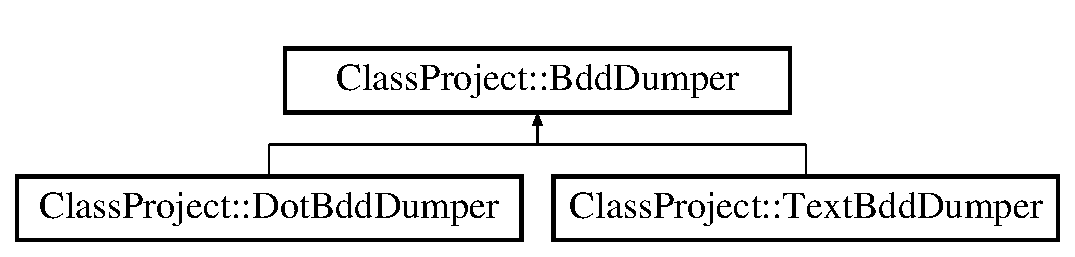
\includegraphics[height=2.000000cm]{classClassProject_1_1BddDumper}
\end{center}
\end{figure}
\subsection*{Public Member Functions}
\begin{DoxyCompactItemize}
\item 
virtual void {\bfseries dump} (const B\+D\+D\+\_\+\+ID \&root, std\+::ostream \&out)=0\label{classClassProject_1_1BddDumper_ae0183004c7f247c8cbc6491de1de5507}

\end{DoxyCompactItemize}


The documentation for this class was generated from the following file\+:\begin{DoxyCompactItemize}
\item 
/home/felipe/\+Desktop/vdsproject/vdscp\+\_\+04/src/bench/Dumper.\+h\end{DoxyCompactItemize}

\section{Class\+Project\+:\+:B\+D\+D\+Hasher Struct Reference}
\label{structClassProject_1_1BDDHasher}\index{Class\+Project\+::\+B\+D\+D\+Hasher@{Class\+Project\+::\+B\+D\+D\+Hasher}}


typedef struct \doxyref{B\+D\+D\+Hasher}{p.}{structClassProject_1_1BDDHasher}  




{\ttfamily \#include $<$Manager.\+h$>$}

\subsection*{Public Member Functions}
\begin{DoxyCompactItemize}
\item 
std\+::size\+\_\+t {\bfseries operator()} (const {\bf B\+D\+D\+\_\+\+Node} \&node) const \label{structClassProject_1_1BDDHasher_accbac47fddd7331f3ec724d314301a69}

\end{DoxyCompactItemize}


\subsection{Detailed Description}
typedef struct \doxyref{B\+D\+D\+Hasher}{p.}{structClassProject_1_1BDDHasher} 

Necessary struct for organizing the elements of the unique\+\_\+table. 

The documentation for this struct was generated from the following file\+:\begin{DoxyCompactItemize}
\item 
/import/home/vdscp04/\+Luiz/vdscp\+\_\+04/src/Manager.\+h\end{DoxyCompactItemize}

\section{Class\+Project\+:\+:Bdd\+Node\+Dumper Class Reference}
\label{classClassProject_1_1BddNodeDumper}\index{Class\+Project\+::\+Bdd\+Node\+Dumper@{Class\+Project\+::\+Bdd\+Node\+Dumper}}
\subsection*{Public Member Functions}
\begin{DoxyCompactItemize}
\item 
virtual void {\bfseries dump} (const B\+D\+D\+\_\+\+ID \&root, std\+::ostream \&out)=0\label{classClassProject_1_1BddNodeDumper_a611562f9f308c185375a6270b603e572}

\end{DoxyCompactItemize}


The documentation for this class was generated from the following file\+:\begin{DoxyCompactItemize}
\item 
/import/home/vdscp04/\+Luiz/vdscp\+\_\+04/src/bench/Dumper.\+h\end{DoxyCompactItemize}

\section{bench\+\_\+circuit\+\_\+manager Class Reference}
\label{classbench__circuit__manager}\index{bench\+\_\+circuit\+\_\+manager@{bench\+\_\+circuit\+\_\+manager}}


Class to convert bench nodes into circuits nodes.  




{\ttfamily \#include $<$bench\+\_\+circuit\+\_\+manager.\+hpp$>$}

\subsection*{Public Member Functions}
\begin{DoxyCompactItemize}
\item 
{\bf bench\+\_\+circuit\+\_\+manager} (std\+::string bench\+\_\+file)
\begin{DoxyCompactList}\small\item\em Constructor. \end{DoxyCompactList}\item 
{\bf $\sim$bench\+\_\+circuit\+\_\+manager} ()
\begin{DoxyCompactList}\small\item\em Destructor. \end{DoxyCompactList}\item 
list\+\_\+of\+\_\+circuit\+\_\+t {\bf Get\+Sorted\+Circuit} (void)
\begin{DoxyCompactList}\small\item\em return the list of circuit nodes topologically sorted. \end{DoxyCompactList}\item 
std\+::set$<$ label\+\_\+t $>$ {\bf Get\+List\+Of\+Output\+Labels} (void)
\begin{DoxyCompactList}\small\item\em return a list with the labels of the O\+U\+T\+P\+UT gates of the circuit. \end{DoxyCompactList}\end{DoxyCompactItemize}


\subsection{Detailed Description}
Class to convert bench nodes into circuits nodes. 

Bench nodes are generated by parsing I\+S\+C\+A\+S85/89/99 bench format files.

\begin{DoxyAuthor}{Authors}
\{Carolina Nogueira\} 
\end{DoxyAuthor}


\subsection{Constructor \& Destructor Documentation}
\index{bench\+\_\+circuit\+\_\+manager@{bench\+\_\+circuit\+\_\+manager}!bench\+\_\+circuit\+\_\+manager@{bench\+\_\+circuit\+\_\+manager}}
\index{bench\+\_\+circuit\+\_\+manager@{bench\+\_\+circuit\+\_\+manager}!bench\+\_\+circuit\+\_\+manager@{bench\+\_\+circuit\+\_\+manager}}
\subsubsection[{bench\+\_\+circuit\+\_\+manager(std\+::string bench\+\_\+file)}]{\setlength{\rightskip}{0pt plus 5cm}bench\+\_\+circuit\+\_\+manager\+::bench\+\_\+circuit\+\_\+manager (
\begin{DoxyParamCaption}
\item[{std\+::string}]{bench\+\_\+file}
\end{DoxyParamCaption}
)}\label{classbench__circuit__manager_a22746f8dacdbe5f5928b795afd409a0e}


Constructor. 


\begin{DoxyParams}{Parameters}
{\em bench\+\_\+file} & is std\+::string. Constructor method for the \doxyref{bench\+\_\+circuit\+\_\+manager}{p.}{classbench__circuit__manager} class. It generates the topological circuit described in the file bench\+\_\+file that must be in the I\+S\+C\+A\+S85/\+I\+S\+C\+A\+S89/\+I\+S\+C\+A\+S99 format. \\
\hline
\end{DoxyParams}
\index{bench\+\_\+circuit\+\_\+manager@{bench\+\_\+circuit\+\_\+manager}!````~bench\+\_\+circuit\+\_\+manager@{$\sim$bench\+\_\+circuit\+\_\+manager}}
\index{````~bench\+\_\+circuit\+\_\+manager@{$\sim$bench\+\_\+circuit\+\_\+manager}!bench\+\_\+circuit\+\_\+manager@{bench\+\_\+circuit\+\_\+manager}}
\subsubsection[{$\sim$bench\+\_\+circuit\+\_\+manager()}]{\setlength{\rightskip}{0pt plus 5cm}bench\+\_\+circuit\+\_\+manager\+::$\sim$bench\+\_\+circuit\+\_\+manager (
\begin{DoxyParamCaption}
{}
\end{DoxyParamCaption}
)}\label{classbench__circuit__manager_a9bae32db63988e78092dbe12563e6f2a}


Destructor. 


\begin{DoxyParams}{Parameters}
{\em none} & Destructor method for the \doxyref{bench\+\_\+circuit\+\_\+manager}{p.}{classbench__circuit__manager} class. \\
\hline
\end{DoxyParams}


References circuit\+\_\+node\+\_\+type\+::gate\+\_\+type, Get\+Sorted\+Circuit(), circuit\+\_\+node\+\_\+type\+::\+ID, circuit\+\_\+node\+\_\+type\+::input\+\_\+\+I\+D\+\_\+list, circuit\+\_\+node\+\_\+type\+::label, and circuit\+\_\+node\+\_\+type\+::output\+\_\+\+I\+D\+\_\+list.



\subsection{Member Function Documentation}
\index{bench\+\_\+circuit\+\_\+manager@{bench\+\_\+circuit\+\_\+manager}!Get\+List\+Of\+Output\+Labels@{Get\+List\+Of\+Output\+Labels}}
\index{Get\+List\+Of\+Output\+Labels@{Get\+List\+Of\+Output\+Labels}!bench\+\_\+circuit\+\_\+manager@{bench\+\_\+circuit\+\_\+manager}}
\subsubsection[{Get\+List\+Of\+Output\+Labels(void)}]{\setlength{\rightskip}{0pt plus 5cm}std\+::set$<$ label\+\_\+t $>$ bench\+\_\+circuit\+\_\+manager\+::\+Get\+List\+Of\+Output\+Labels (
\begin{DoxyParamCaption}
\item[{void}]{}
\end{DoxyParamCaption}
)}\label{classbench__circuit__manager_a5459b47ba3b32b1a0a6a4de8cdf22ad6}


return a list with the labels of the O\+U\+T\+P\+UT gates of the circuit. 

The label\textquotesingle{}s list also includes the F\+L\+I\+P\+\_\+\+F\+L\+O\+PS 
\begin{DoxyParams}{Parameters}
{\em none} & \\
\hline
\end{DoxyParams}
\begin{DoxyReturn}{Returns}
std\+::set$<$label\+\_\+t$>$ 
\end{DoxyReturn}
\index{bench\+\_\+circuit\+\_\+manager@{bench\+\_\+circuit\+\_\+manager}!Get\+Sorted\+Circuit@{Get\+Sorted\+Circuit}}
\index{Get\+Sorted\+Circuit@{Get\+Sorted\+Circuit}!bench\+\_\+circuit\+\_\+manager@{bench\+\_\+circuit\+\_\+manager}}
\subsubsection[{Get\+Sorted\+Circuit(void)}]{\setlength{\rightskip}{0pt plus 5cm}list\+\_\+of\+\_\+circuit\+\_\+t bench\+\_\+circuit\+\_\+manager\+::\+Get\+Sorted\+Circuit (
\begin{DoxyParamCaption}
\item[{void}]{}
\end{DoxyParamCaption}
)}\label{classbench__circuit__manager_ab2c34fc07b9f3fe4591cede486b7ad17}


return the list of circuit nodes topologically sorted. 


\begin{DoxyParams}{Parameters}
{\em none} & \\
\hline
\end{DoxyParams}
\begin{DoxyReturn}{Returns}
list\+\_\+of\+\_\+circuit\+\_\+t 
\end{DoxyReturn}


References circuit\+\_\+node\+\_\+type\+::gate\+\_\+type, circuit\+\_\+node\+\_\+type\+::\+ID, circuit\+\_\+node\+\_\+type\+::input\+\_\+\+I\+D\+\_\+list, and circuit\+\_\+node\+\_\+type\+::label.



Referenced by $\sim$bench\+\_\+circuit\+\_\+manager().



The documentation for this class was generated from the following files\+:\begin{DoxyCompactItemize}
\item 
/import/home/vdscp04/\+Luiz/vdscp\+\_\+04/src/bench/bench\+\_\+circuit\+\_\+manager.\+hpp\item 
/import/home/vdscp04/\+Luiz/vdscp\+\_\+04/src/bench/bench\+\_\+circuit\+\_\+manager.\+cpp\end{DoxyCompactItemize}

\section{bench\+\_\+format\+:\+:bench\+\_\+node\+\_\+type Struct Reference}
\label{structbench__format_1_1bench__node__type}\index{bench\+\_\+format\+::bench\+\_\+node\+\_\+type@{bench\+\_\+format\+::bench\+\_\+node\+\_\+type}}
\subsection*{Public Attributes}
\begin{DoxyCompactItemize}
\item 
std\+::string {\bfseries label}\label{structbench__format_1_1bench__node__type_ad84a489da088407c9eef963e35632b32}

\item 
std\+::string {\bfseries gate\+\_\+type}\label{structbench__format_1_1bench__node__type_aa6ff9b16997a95578623b93302abad12}

\item 
std\+::vector$<$ std\+::string $>$ {\bfseries input\+\_\+node\+\_\+list}\label{structbench__format_1_1bench__node__type_a006ef045067295870a13b146ebc10e52}

\end{DoxyCompactItemize}


The documentation for this struct was generated from the following file\+:\begin{DoxyCompactItemize}
\item 
/import/home/vdscp04/\+Luiz/vdscp\+\_\+04/src/bench/bench\+\_\+grammar.\+hpp\end{DoxyCompactItemize}

\section{Cicle\+Exception Class Reference}
\label{classCicleException}\index{Cicle\+Exception@{Cicle\+Exception}}


This exception should be thrown when a non-\/cycle free circuit is parsed.  




{\ttfamily \#include $<$bench\+\_\+circuit\+\_\+manager.\+hpp$>$}

Inheritance diagram for Cicle\+Exception\+:\begin{figure}[H]
\begin{center}
\leavevmode
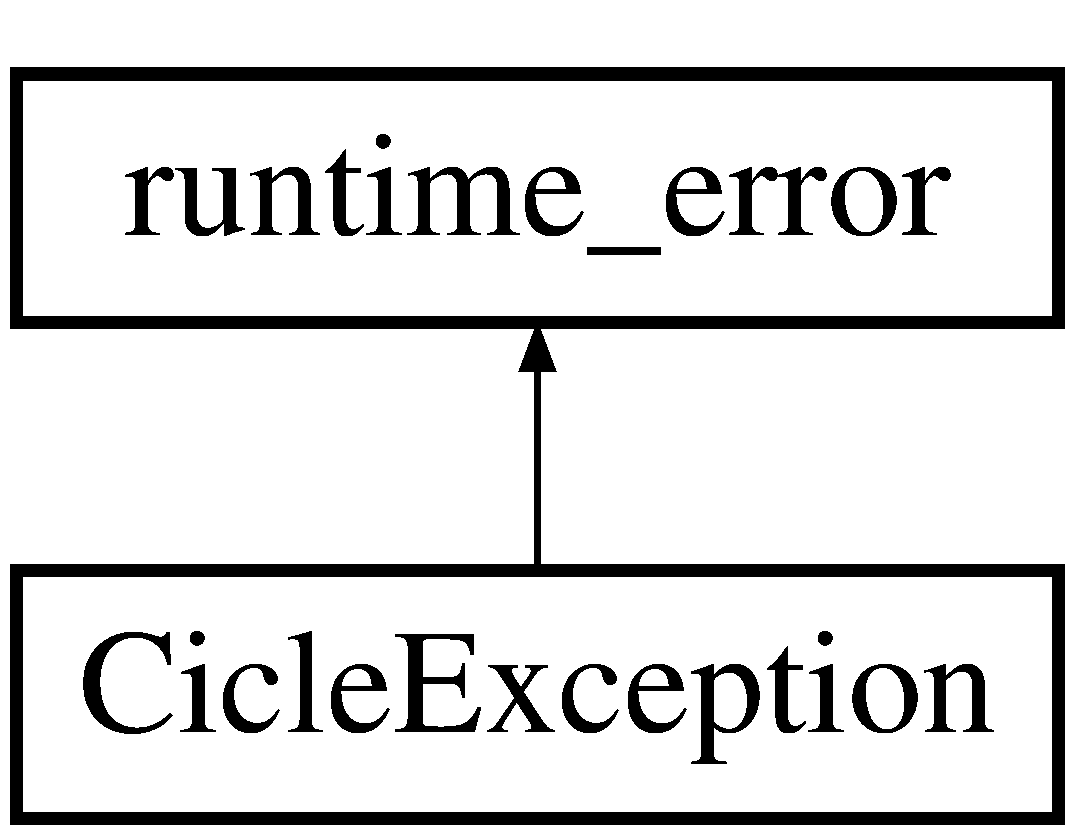
\includegraphics[height=2.000000cm]{classCicleException}
\end{center}
\end{figure}
\subsection*{Public Member Functions}
\begin{DoxyCompactItemize}
\item 
{\bfseries Cicle\+Exception} (const std\+::string \&message)\label{classCicleException_a51147b615bdb26f9301f0a79bba60c28}

\end{DoxyCompactItemize}


\subsection{Detailed Description}
This exception should be thrown when a non-\/cycle free circuit is parsed. 

The documentation for this class was generated from the following file\+:\begin{DoxyCompactItemize}
\item 
/import/home/vdscp04/\+Luiz/vdscp\+\_\+04/src/bench/bench\+\_\+circuit\+\_\+manager.\+hpp\end{DoxyCompactItemize}

\section{circuit\+\_\+node\+\_\+type Struct Reference}
\label{structcircuit__node__type}\index{circuit\+\_\+node\+\_\+type@{circuit\+\_\+node\+\_\+type}}


Struct that represents a node from a circuit.  




{\ttfamily \#include $<$bench\+\_\+circuit\+\_\+manager.\+hpp$>$}

\subsection*{Public Attributes}
\begin{DoxyCompactItemize}
\item 
unique\+\_\+\+I\+D\+\_\+t {\bf ID}\label{structcircuit__node__type_afacb1e6847ed44fac3331f71f5ec04b6}

\begin{DoxyCompactList}\small\item\em Unique ID for a node. \end{DoxyCompactList}\item 
std\+::string {\bf label}\label{structcircuit__node__type_af8938c10e6a23cf894a7fa8c7ed1418c}

\begin{DoxyCompactList}\small\item\em Node Label. \end{DoxyCompactList}\item 
std\+::string {\bf gate\+\_\+type}\label{structcircuit__node__type_a6d3b4331c5ad9a248154bfbada6ef9df}

\begin{DoxyCompactList}\small\item\em Type of the gate (ex. A\+ND, N\+OT, OR) \end{DoxyCompactList}\item 
set\+\_\+of\+\_\+circuit\+\_\+t {\bf input\+\_\+\+I\+D\+\_\+list}\label{structcircuit__node__type_a569f94035014dfc750d4070aee13876e}

\begin{DoxyCompactList}\small\item\em set containing all the inputs of the respective gate \end{DoxyCompactList}\item 
set\+\_\+of\+\_\+circuit\+\_\+t {\bf output\+\_\+\+I\+D\+\_\+list}\label{structcircuit__node__type_abeef1f2b534968593864f1193c964660}

\begin{DoxyCompactList}\small\item\em set containing all the outputs of the respective gate \end{DoxyCompactList}\end{DoxyCompactItemize}


\subsection{Detailed Description}
Struct that represents a node from a circuit. 

The documentation for this struct was generated from the following file\+:\begin{DoxyCompactItemize}
\item 
/import/home/vdscp04/\+Luiz/vdscp\+\_\+04/src/bench/bench\+\_\+circuit\+\_\+manager.\+hpp\end{DoxyCompactItemize}

\section{circuit\+\_\+to\+\_\+\+B\+D\+D\+\_\+manager Class Reference}
\label{classcircuit__to__BDD__manager}\index{circuit\+\_\+to\+\_\+\+B\+D\+D\+\_\+manager@{circuit\+\_\+to\+\_\+\+B\+D\+D\+\_\+manager}}


Class to convert circuits nodes into B\+DD nodes.  




{\ttfamily \#include $<$circuit\+\_\+to\+\_\+\+B\+D\+D\+\_\+manager.\+hpp$>$}

\subsection*{Public Member Functions}
\begin{DoxyCompactItemize}
\item 
{\bf circuit\+\_\+to\+\_\+\+B\+D\+D\+\_\+manager} ({\bf Class\+Project\+::\+Manager\+Interface} $\ast$B\+D\+D\+\_\+manager\+\_\+iface)
\begin{DoxyCompactList}\small\item\em Constructor. \end{DoxyCompactList}\item 
{\bf $\sim$circuit\+\_\+to\+\_\+\+B\+D\+D\+\_\+manager} ()
\begin{DoxyCompactList}\small\item\em Destructor. \end{DoxyCompactList}\item 
void {\bf Generate\+B\+DD} (list\+\_\+of\+\_\+circuit\+\_\+t circuit, std\+::string benchmark\+\_\+file)
\begin{DoxyCompactList}\small\item\em generates B\+DD from the circuit nodes provided. \end{DoxyCompactList}\item 
void {\bfseries Print\+B\+DD} (std\+::set$<$ label\+\_\+t $>$ set\+\_\+of\+\_\+output\+\_\+labels)\label{classcircuit__to__BDD__manager_acfd5ec2277046cc7b1c78d5f43e18802}

\end{DoxyCompactItemize}
\subsection*{Private Member Functions}
\begin{DoxyCompactItemize}
\item 
Class\+Project\+::\+B\+D\+D\+\_\+\+ID {\bf circuit\+Id2\+B\+D\+Did} (unique\+\_\+\+I\+D\+\_\+t {\bf node})
\begin{DoxyCompactList}\small\item\em returns the B\+D\+D\+\_\+\+ID of the given circuit ID. \end{DoxyCompactList}\item 
Class\+Project\+::\+B\+D\+D\+\_\+\+ID {\bf Input\+Gate} (label\+\_\+t label)
\begin{DoxyCompactList}\small\item\em generates the B\+DD node equivalent to a variable with label \char`\"{}label\char`\"{}. \end{DoxyCompactList}\item 
Class\+Project\+::\+B\+D\+D\+\_\+\+ID {\bf Not\+Gate} (set\+\_\+of\+\_\+circuit\+\_\+t {\bf node})
\begin{DoxyCompactList}\small\item\em generates the B\+DD node equivalent to the N\+OT gate. \end{DoxyCompactList}\item 
Class\+Project\+::\+B\+D\+D\+\_\+\+ID {\bf And\+Gate} (set\+\_\+of\+\_\+circuit\+\_\+t input\+Nodes)
\begin{DoxyCompactList}\small\item\em generates the B\+DD node equivalent to the A\+ND gate. \end{DoxyCompactList}\item 
Class\+Project\+::\+B\+D\+D\+\_\+\+ID {\bf Or\+Gate} (set\+\_\+of\+\_\+circuit\+\_\+t input\+Nodes)
\begin{DoxyCompactList}\small\item\em generates the B\+DD node equivalent to the OR gate. \end{DoxyCompactList}\item 
Class\+Project\+::\+B\+D\+D\+\_\+\+ID {\bf Nand\+Gate} (set\+\_\+of\+\_\+circuit\+\_\+t input\+Nodes)
\begin{DoxyCompactList}\small\item\em generates the B\+DD node equivalent to the N\+A\+ND gate. \end{DoxyCompactList}\item 
Class\+Project\+::\+B\+D\+D\+\_\+\+ID {\bf Nor\+Gate} (set\+\_\+of\+\_\+circuit\+\_\+t input\+Nodes)
\begin{DoxyCompactList}\small\item\em generates the B\+DD node equivalent to the N\+OR gate. \end{DoxyCompactList}\item 
Class\+Project\+::\+B\+D\+D\+\_\+\+ID {\bf Xor\+Gate} (set\+\_\+of\+\_\+circuit\+\_\+t input\+Nodes)
\begin{DoxyCompactList}\small\item\em generates the B\+DD node equivalent to the X\+OR gate. \end{DoxyCompactList}\end{DoxyCompactItemize}
\subsection*{Private Attributes}
\begin{DoxyCompactItemize}
\item 
boost\+::unordered\+\_\+map$<$ unique\+\_\+\+I\+D\+\_\+t, Class\+Project\+::\+B\+D\+D\+\_\+\+ID $>$ {\bf node2\+B\+D\+D\+Table}\label{classcircuit__to__BDD__manager_aa04b91e7e456181a61e99662481906bc}

\begin{DoxyCompactList}\small\item\em Mapping from circuit node unique I\+Ds to B\+DD I\+Ds. \end{DoxyCompactList}\item 
std\+::unordered\+\_\+map$<$ label\+\_\+t, Class\+Project\+::\+B\+D\+D\+\_\+\+ID $>$ {\bf label2\+B\+D\+D\+\_\+\+I\+D\+\_\+table}\label{classcircuit__to__BDD__manager_aa499154088871f0b80df5479f906eb7f}

\begin{DoxyCompactList}\small\item\em Mapping from node\textquotesingle{}s label to B\+DD I\+Ds. \end{DoxyCompactList}\item 
{\bf Class\+Project\+::\+Manager\+Interface} $\ast$ {\bfseries B\+D\+D\+\_\+manager}\label{classcircuit__to__BDD__manager_ad327024d0703a4919ca14aef79798d3a}

\item 
std\+::string {\bf result\+\_\+dir}\label{classcircuit__to__BDD__manager_a3d565b303c29cb8b8ec6b886625c532d}

\begin{DoxyCompactList}\small\item\em Directory where the results are stored. \end{DoxyCompactList}\end{DoxyCompactItemize}


\subsection{Detailed Description}
Class to convert circuits nodes into B\+DD nodes. 

Circuit nodes are generated by the class \doxyref{bench\+\_\+circuit\+\_\+manager}{p.}{classbench__circuit__manager}.

\begin{DoxyAuthor}{Authors}
\{Carolina Nogueira\} 
\end{DoxyAuthor}


\subsection{Constructor \& Destructor Documentation}
\index{circuit\+\_\+to\+\_\+\+B\+D\+D\+\_\+manager@{circuit\+\_\+to\+\_\+\+B\+D\+D\+\_\+manager}!circuit\+\_\+to\+\_\+\+B\+D\+D\+\_\+manager@{circuit\+\_\+to\+\_\+\+B\+D\+D\+\_\+manager}}
\index{circuit\+\_\+to\+\_\+\+B\+D\+D\+\_\+manager@{circuit\+\_\+to\+\_\+\+B\+D\+D\+\_\+manager}!circuit\+\_\+to\+\_\+\+B\+D\+D\+\_\+manager@{circuit\+\_\+to\+\_\+\+B\+D\+D\+\_\+manager}}
\subsubsection[{circuit\+\_\+to\+\_\+\+B\+D\+D\+\_\+manager(\+Class\+Project\+::\+Manager\+Interface $\ast$\+B\+D\+D\+\_\+manager\+\_\+iface)}]{\setlength{\rightskip}{0pt plus 5cm}circuit\+\_\+to\+\_\+\+B\+D\+D\+\_\+manager\+::circuit\+\_\+to\+\_\+\+B\+D\+D\+\_\+manager (
\begin{DoxyParamCaption}
\item[{{\bf Class\+Project\+::\+Manager\+Interface} $\ast$}]{B\+D\+D\+\_\+manager\+\_\+iface}
\end{DoxyParamCaption}
)}\label{classcircuit__to__BDD__manager_a0d38bd20427387145177f4aa20ba08ca}


Constructor. 


\begin{DoxyParams}{Parameters}
{\em B\+D\+D\+\_\+manager\+\_\+iface} & is \doxyref{Class\+Project\+::\+Manager\+Interface}{p.}{classClassProject_1_1ManagerInterface} Constructor method for the \doxyref{circuit\+\_\+to\+\_\+\+B\+D\+D\+\_\+manager}{p.}{classcircuit__to__BDD__manager} class. \\
\hline
\end{DoxyParams}
\index{circuit\+\_\+to\+\_\+\+B\+D\+D\+\_\+manager@{circuit\+\_\+to\+\_\+\+B\+D\+D\+\_\+manager}!````~circuit\+\_\+to\+\_\+\+B\+D\+D\+\_\+manager@{$\sim$circuit\+\_\+to\+\_\+\+B\+D\+D\+\_\+manager}}
\index{````~circuit\+\_\+to\+\_\+\+B\+D\+D\+\_\+manager@{$\sim$circuit\+\_\+to\+\_\+\+B\+D\+D\+\_\+manager}!circuit\+\_\+to\+\_\+\+B\+D\+D\+\_\+manager@{circuit\+\_\+to\+\_\+\+B\+D\+D\+\_\+manager}}
\subsubsection[{$\sim$circuit\+\_\+to\+\_\+\+B\+D\+D\+\_\+manager()}]{\setlength{\rightskip}{0pt plus 5cm}circuit\+\_\+to\+\_\+\+B\+D\+D\+\_\+manager\+::$\sim$circuit\+\_\+to\+\_\+\+B\+D\+D\+\_\+manager (
\begin{DoxyParamCaption}
{}
\end{DoxyParamCaption}
)}\label{classcircuit__to__BDD__manager_a18751e8a0a28c61a84a576fc3d565b78}


Destructor. 


\begin{DoxyParams}{Parameters}
{\em none} & Destructor method for the \doxyref{circuit\+\_\+to\+\_\+\+B\+D\+D\+\_\+manager}{p.}{classcircuit__to__BDD__manager} class. \\
\hline
\end{DoxyParams}


\subsection{Member Function Documentation}
\index{circuit\+\_\+to\+\_\+\+B\+D\+D\+\_\+manager@{circuit\+\_\+to\+\_\+\+B\+D\+D\+\_\+manager}!And\+Gate@{And\+Gate}}
\index{And\+Gate@{And\+Gate}!circuit\+\_\+to\+\_\+\+B\+D\+D\+\_\+manager@{circuit\+\_\+to\+\_\+\+B\+D\+D\+\_\+manager}}
\subsubsection[{And\+Gate(set\+\_\+of\+\_\+circuit\+\_\+t input\+Nodes)}]{\setlength{\rightskip}{0pt plus 5cm}Class\+Project\+::\+B\+D\+D\+\_\+\+ID circuit\+\_\+to\+\_\+\+B\+D\+D\+\_\+manager\+::\+And\+Gate (
\begin{DoxyParamCaption}
\item[{set\+\_\+of\+\_\+circuit\+\_\+t}]{input\+Nodes}
\end{DoxyParamCaption}
)\hspace{0.3cm}{\ttfamily [private]}}\label{classcircuit__to__BDD__manager_ae42b3652550e68a09a785f5c1b8f63de}


generates the B\+DD node equivalent to the A\+ND gate. 


\begin{DoxyParams}{Parameters}
{\em node} & is set\+\_\+of\+\_\+circuit\+\_\+t containing the circuit I\+Ds of the gates to be used as input. \\
\hline
\end{DoxyParams}
\begin{DoxyReturn}{Returns}
Class\+Project\+::\+B\+D\+D\+\_\+\+ID 
\end{DoxyReturn}


References circuit\+Id2\+B\+D\+Did().



Referenced by Generate\+B\+D\+D(), and Nand\+Gate().

\index{circuit\+\_\+to\+\_\+\+B\+D\+D\+\_\+manager@{circuit\+\_\+to\+\_\+\+B\+D\+D\+\_\+manager}!circuit\+Id2\+B\+D\+Did@{circuit\+Id2\+B\+D\+Did}}
\index{circuit\+Id2\+B\+D\+Did@{circuit\+Id2\+B\+D\+Did}!circuit\+\_\+to\+\_\+\+B\+D\+D\+\_\+manager@{circuit\+\_\+to\+\_\+\+B\+D\+D\+\_\+manager}}
\subsubsection[{circuit\+Id2\+B\+D\+Did(unique\+\_\+\+I\+D\+\_\+t node)}]{\setlength{\rightskip}{0pt plus 5cm}Class\+Project\+::\+B\+D\+D\+\_\+\+ID circuit\+\_\+to\+\_\+\+B\+D\+D\+\_\+manager\+::circuit\+Id2\+B\+D\+Did (
\begin{DoxyParamCaption}
\item[{unique\+\_\+\+I\+D\+\_\+t}]{node}
\end{DoxyParamCaption}
)\hspace{0.3cm}{\ttfamily [private]}}\label{classcircuit__to__BDD__manager_a4b6d8e87f4cba8ef146d4ae37b5924c1}


returns the B\+D\+D\+\_\+\+ID of the given circuit ID. 


\begin{DoxyParams}{Parameters}
{\em node} & is unique\+\_\+\+I\+D\+\_\+t \\
\hline
\end{DoxyParams}
\begin{DoxyReturn}{Returns}
Class\+Project\+::\+B\+D\+D\+\_\+\+ID 
\end{DoxyReturn}


References node2\+B\+D\+D\+Table.



Referenced by And\+Gate(), Generate\+B\+D\+D(), Nand\+Gate(), Nor\+Gate(), Not\+Gate(), Or\+Gate(), and Xor\+Gate().

\index{circuit\+\_\+to\+\_\+\+B\+D\+D\+\_\+manager@{circuit\+\_\+to\+\_\+\+B\+D\+D\+\_\+manager}!Generate\+B\+DD@{Generate\+B\+DD}}
\index{Generate\+B\+DD@{Generate\+B\+DD}!circuit\+\_\+to\+\_\+\+B\+D\+D\+\_\+manager@{circuit\+\_\+to\+\_\+\+B\+D\+D\+\_\+manager}}
\subsubsection[{Generate\+B\+D\+D(list\+\_\+of\+\_\+circuit\+\_\+t circuit, std\+::string benchmark\+\_\+file)}]{\setlength{\rightskip}{0pt plus 5cm}void circuit\+\_\+to\+\_\+\+B\+D\+D\+\_\+manager\+::\+Generate\+B\+DD (
\begin{DoxyParamCaption}
\item[{list\+\_\+of\+\_\+circuit\+\_\+t}]{circuit, }
\item[{std\+::string}]{benchmark\+\_\+file}
\end{DoxyParamCaption}
)}\label{classcircuit__to__BDD__manager_ae1b5244f8b77673ccaef57b70b10c0d6}


generates B\+DD from the circuit nodes provided. 


\begin{DoxyParams}{Parameters}
{\em circuit} & is list\+\_\+of\+\_\+circuit\+\_\+t -\/ topologic sorted list containing the circuit nodes \\
\hline
\end{DoxyParams}
\begin{DoxyReturn}{Returns}
none
\end{DoxyReturn}
Generates the calls to the B\+DD package in order to generate the B\+DD equivalent to the provided circuit. 

References And\+Gate(), circuit\+Id2\+B\+D\+Did(), Input\+Gate(), label2\+B\+D\+D\+\_\+\+I\+D\+\_\+table, Nand\+Gate(), node2\+B\+D\+D\+Table, Nor\+Gate(), Not\+Gate(), Or\+Gate(), result\+\_\+dir, and Xor\+Gate().

\index{circuit\+\_\+to\+\_\+\+B\+D\+D\+\_\+manager@{circuit\+\_\+to\+\_\+\+B\+D\+D\+\_\+manager}!Input\+Gate@{Input\+Gate}}
\index{Input\+Gate@{Input\+Gate}!circuit\+\_\+to\+\_\+\+B\+D\+D\+\_\+manager@{circuit\+\_\+to\+\_\+\+B\+D\+D\+\_\+manager}}
\subsubsection[{Input\+Gate(label\+\_\+t label)}]{\setlength{\rightskip}{0pt plus 5cm}Class\+Project\+::\+B\+D\+D\+\_\+\+ID circuit\+\_\+to\+\_\+\+B\+D\+D\+\_\+manager\+::\+Input\+Gate (
\begin{DoxyParamCaption}
\item[{label\+\_\+t}]{label}
\end{DoxyParamCaption}
)\hspace{0.3cm}{\ttfamily [private]}}\label{classcircuit__to__BDD__manager_a027d557393d1d33b7cecdf593489956e}


generates the B\+DD node equivalent to a variable with label \char`\"{}label\char`\"{}. 


\begin{DoxyParams}{Parameters}
{\em label} & is label\+\_\+t \\
\hline
\end{DoxyParams}
\begin{DoxyReturn}{Returns}
Class\+Project\+::\+B\+D\+D\+\_\+\+ID 
\end{DoxyReturn}


Referenced by Generate\+B\+D\+D().

\index{circuit\+\_\+to\+\_\+\+B\+D\+D\+\_\+manager@{circuit\+\_\+to\+\_\+\+B\+D\+D\+\_\+manager}!Nand\+Gate@{Nand\+Gate}}
\index{Nand\+Gate@{Nand\+Gate}!circuit\+\_\+to\+\_\+\+B\+D\+D\+\_\+manager@{circuit\+\_\+to\+\_\+\+B\+D\+D\+\_\+manager}}
\subsubsection[{Nand\+Gate(set\+\_\+of\+\_\+circuit\+\_\+t input\+Nodes)}]{\setlength{\rightskip}{0pt plus 5cm}Class\+Project\+::\+B\+D\+D\+\_\+\+ID circuit\+\_\+to\+\_\+\+B\+D\+D\+\_\+manager\+::\+Nand\+Gate (
\begin{DoxyParamCaption}
\item[{set\+\_\+of\+\_\+circuit\+\_\+t}]{input\+Nodes}
\end{DoxyParamCaption}
)\hspace{0.3cm}{\ttfamily [private]}}\label{classcircuit__to__BDD__manager_a9cbe6a7e2e3264978476f8a060f104f5}


generates the B\+DD node equivalent to the N\+A\+ND gate. 


\begin{DoxyParams}{Parameters}
{\em node} & is set\+\_\+of\+\_\+circuit\+\_\+t containing the circuit I\+Ds of the gates to be used as input. \\
\hline
\end{DoxyParams}
\begin{DoxyReturn}{Returns}
Class\+Project\+::\+B\+D\+D\+\_\+\+ID 
\end{DoxyReturn}


References And\+Gate(), and circuit\+Id2\+B\+D\+Did().



Referenced by Generate\+B\+D\+D().

\index{circuit\+\_\+to\+\_\+\+B\+D\+D\+\_\+manager@{circuit\+\_\+to\+\_\+\+B\+D\+D\+\_\+manager}!Nor\+Gate@{Nor\+Gate}}
\index{Nor\+Gate@{Nor\+Gate}!circuit\+\_\+to\+\_\+\+B\+D\+D\+\_\+manager@{circuit\+\_\+to\+\_\+\+B\+D\+D\+\_\+manager}}
\subsubsection[{Nor\+Gate(set\+\_\+of\+\_\+circuit\+\_\+t input\+Nodes)}]{\setlength{\rightskip}{0pt plus 5cm}Class\+Project\+::\+B\+D\+D\+\_\+\+ID circuit\+\_\+to\+\_\+\+B\+D\+D\+\_\+manager\+::\+Nor\+Gate (
\begin{DoxyParamCaption}
\item[{set\+\_\+of\+\_\+circuit\+\_\+t}]{input\+Nodes}
\end{DoxyParamCaption}
)\hspace{0.3cm}{\ttfamily [private]}}\label{classcircuit__to__BDD__manager_ac5b3c1a35ca431c955183ed9df72cf8b}


generates the B\+DD node equivalent to the N\+OR gate. 


\begin{DoxyParams}{Parameters}
{\em node} & is set\+\_\+of\+\_\+circuit\+\_\+t containing the circuit I\+Ds of the gates to be used as input. \\
\hline
\end{DoxyParams}
\begin{DoxyReturn}{Returns}
Class\+Project\+::\+B\+D\+D\+\_\+\+ID 
\end{DoxyReturn}


References circuit\+Id2\+B\+D\+Did(), and Or\+Gate().



Referenced by Generate\+B\+D\+D().

\index{circuit\+\_\+to\+\_\+\+B\+D\+D\+\_\+manager@{circuit\+\_\+to\+\_\+\+B\+D\+D\+\_\+manager}!Not\+Gate@{Not\+Gate}}
\index{Not\+Gate@{Not\+Gate}!circuit\+\_\+to\+\_\+\+B\+D\+D\+\_\+manager@{circuit\+\_\+to\+\_\+\+B\+D\+D\+\_\+manager}}
\subsubsection[{Not\+Gate(set\+\_\+of\+\_\+circuit\+\_\+t node)}]{\setlength{\rightskip}{0pt plus 5cm}Class\+Project\+::\+B\+D\+D\+\_\+\+ID circuit\+\_\+to\+\_\+\+B\+D\+D\+\_\+manager\+::\+Not\+Gate (
\begin{DoxyParamCaption}
\item[{set\+\_\+of\+\_\+circuit\+\_\+t}]{node}
\end{DoxyParamCaption}
)\hspace{0.3cm}{\ttfamily [private]}}\label{classcircuit__to__BDD__manager_a8bafb05dc7df4a67173b4997b2fb402d}


generates the B\+DD node equivalent to the N\+OT gate. 


\begin{DoxyParams}{Parameters}
{\em node} & is set\+\_\+of\+\_\+circuit\+\_\+t containing the circuit ID of the gate to be inverted. \\
\hline
\end{DoxyParams}
\begin{DoxyReturn}{Returns}
Class\+Project\+::\+B\+D\+D\+\_\+\+ID 
\end{DoxyReturn}


References circuit\+Id2\+B\+D\+Did().



Referenced by Generate\+B\+D\+D().

\index{circuit\+\_\+to\+\_\+\+B\+D\+D\+\_\+manager@{circuit\+\_\+to\+\_\+\+B\+D\+D\+\_\+manager}!Or\+Gate@{Or\+Gate}}
\index{Or\+Gate@{Or\+Gate}!circuit\+\_\+to\+\_\+\+B\+D\+D\+\_\+manager@{circuit\+\_\+to\+\_\+\+B\+D\+D\+\_\+manager}}
\subsubsection[{Or\+Gate(set\+\_\+of\+\_\+circuit\+\_\+t input\+Nodes)}]{\setlength{\rightskip}{0pt plus 5cm}Class\+Project\+::\+B\+D\+D\+\_\+\+ID circuit\+\_\+to\+\_\+\+B\+D\+D\+\_\+manager\+::\+Or\+Gate (
\begin{DoxyParamCaption}
\item[{set\+\_\+of\+\_\+circuit\+\_\+t}]{input\+Nodes}
\end{DoxyParamCaption}
)\hspace{0.3cm}{\ttfamily [private]}}\label{classcircuit__to__BDD__manager_a2bfb5bf2686e20a65b63109f73d2c8aa}


generates the B\+DD node equivalent to the OR gate. 


\begin{DoxyParams}{Parameters}
{\em node} & is set\+\_\+of\+\_\+circuit\+\_\+t containing the circuit I\+Ds of the gates to be used as input. \\
\hline
\end{DoxyParams}
\begin{DoxyReturn}{Returns}
Class\+Project\+::\+B\+D\+D\+\_\+\+ID 
\end{DoxyReturn}


References circuit\+Id2\+B\+D\+Did().



Referenced by Generate\+B\+D\+D(), and Nor\+Gate().

\index{circuit\+\_\+to\+\_\+\+B\+D\+D\+\_\+manager@{circuit\+\_\+to\+\_\+\+B\+D\+D\+\_\+manager}!Xor\+Gate@{Xor\+Gate}}
\index{Xor\+Gate@{Xor\+Gate}!circuit\+\_\+to\+\_\+\+B\+D\+D\+\_\+manager@{circuit\+\_\+to\+\_\+\+B\+D\+D\+\_\+manager}}
\subsubsection[{Xor\+Gate(set\+\_\+of\+\_\+circuit\+\_\+t input\+Nodes)}]{\setlength{\rightskip}{0pt plus 5cm}Class\+Project\+::\+B\+D\+D\+\_\+\+ID circuit\+\_\+to\+\_\+\+B\+D\+D\+\_\+manager\+::\+Xor\+Gate (
\begin{DoxyParamCaption}
\item[{set\+\_\+of\+\_\+circuit\+\_\+t}]{input\+Nodes}
\end{DoxyParamCaption}
)\hspace{0.3cm}{\ttfamily [private]}}\label{classcircuit__to__BDD__manager_ac8140f284db475fca0c3d0aea379bdee}


generates the B\+DD node equivalent to the X\+OR gate. 


\begin{DoxyParams}{Parameters}
{\em node} & is set\+\_\+of\+\_\+circuit\+\_\+t containing the circuit I\+Ds of the gates to be used as input. \\
\hline
\end{DoxyParams}
\begin{DoxyReturn}{Returns}
Class\+Project\+::\+B\+D\+D\+\_\+\+ID 
\end{DoxyReturn}


References circuit\+Id2\+B\+D\+Did(), label2\+B\+D\+D\+\_\+\+I\+D\+\_\+table, and result\+\_\+dir.



Referenced by Generate\+B\+D\+D().



The documentation for this class was generated from the following files\+:\begin{DoxyCompactItemize}
\item 
/home/felipe/\+Desktop/vdsproject/vdscp\+\_\+04/src/bench/circuit\+\_\+to\+\_\+\+B\+D\+D\+\_\+manager.\+hpp\item 
/home/felipe/\+Desktop/vdsproject/vdscp\+\_\+04/src/bench/circuit\+\_\+to\+\_\+\+B\+D\+D\+\_\+manager.\+cpp\end{DoxyCompactItemize}

\section{ska\+:\+:detailv3\+:\+:sherwood\+\_\+v3\+\_\+table$<$ T, Find\+Key, Argument\+Hash, Hasher, Argument\+Equal, Equal, Argument\+Alloc, Entry\+Alloc $>$\+:\+:convertible\+\_\+to\+\_\+iterator Struct Reference}
\label{structska_1_1detailv3_1_1sherwood__v3__table_1_1convertible__to__iterator}\index{ska\+::detailv3\+::sherwood\+\_\+v3\+\_\+table$<$ T, Find\+Key, Argument\+Hash, Hasher, Argument\+Equal, Equal, Argument\+Alloc, Entry\+Alloc $>$\+::convertible\+\_\+to\+\_\+iterator@{ska\+::detailv3\+::sherwood\+\_\+v3\+\_\+table$<$ T, Find\+Key, Argument\+Hash, Hasher, Argument\+Equal, Equal, Argument\+Alloc, Entry\+Alloc $>$\+::convertible\+\_\+to\+\_\+iterator}}
\subsection*{Public Member Functions}
\begin{DoxyCompactItemize}
\item 
{\bfseries operator iterator} ()\label{structska_1_1detailv3_1_1sherwood__v3__table_1_1convertible__to__iterator_a07b15b09cfd1165e125dab6dcb5225f0}

\item 
{\bfseries operator const\+\_\+iterator} ()\label{structska_1_1detailv3_1_1sherwood__v3__table_1_1convertible__to__iterator_a27528469b747c52bbf018039cdfac1f7}

\end{DoxyCompactItemize}
\subsection*{Public Attributes}
\begin{DoxyCompactItemize}
\item 
Entry\+Pointer {\bfseries it}\label{structska_1_1detailv3_1_1sherwood__v3__table_1_1convertible__to__iterator_adacc35f9cf624553e7ca30553f529295}

\end{DoxyCompactItemize}


The documentation for this struct was generated from the following file\+:\begin{DoxyCompactItemize}
\item 
/home/felipe/\+Desktop/vdsproject/vdscp\+\_\+04/src/flat\+\_\+hash\+\_\+map.\+hpp\end{DoxyCompactItemize}

\section{ska\+:\+:flat\+\_\+hash\+\_\+map$<$ K, V, H, E, A $>$\+:\+:convertible\+\_\+to\+\_\+value Struct Reference}
\label{structska_1_1flat__hash__map_1_1convertible__to__value}\index{ska\+::flat\+\_\+hash\+\_\+map$<$ K, V, H, E, A $>$\+::convertible\+\_\+to\+\_\+value@{ska\+::flat\+\_\+hash\+\_\+map$<$ K, V, H, E, A $>$\+::convertible\+\_\+to\+\_\+value}}
\subsection*{Public Member Functions}
\begin{DoxyCompactItemize}
\item 
{\bfseries operator V} () const \label{structska_1_1flat__hash__map_1_1convertible__to__value_ab571586a204b0d1d43df564d730b453e}

\end{DoxyCompactItemize}


The documentation for this struct was generated from the following file\+:\begin{DoxyCompactItemize}
\item 
/home/felipe/\+Desktop/vdsproject/vdscp\+\_\+04/src/flat\+\_\+hash\+\_\+map.\+hpp\end{DoxyCompactItemize}

\section{Dir\+Exception Class Reference}
\label{classDirException}\index{Dir\+Exception@{Dir\+Exception}}


This exception should be thrown when it is not possible create a directory.  




{\ttfamily \#include $<$circuit\+\_\+to\+\_\+\+B\+D\+D\+\_\+manager.\+hpp$>$}

Inheritance diagram for Dir\+Exception\+:\begin{figure}[H]
\begin{center}
\leavevmode
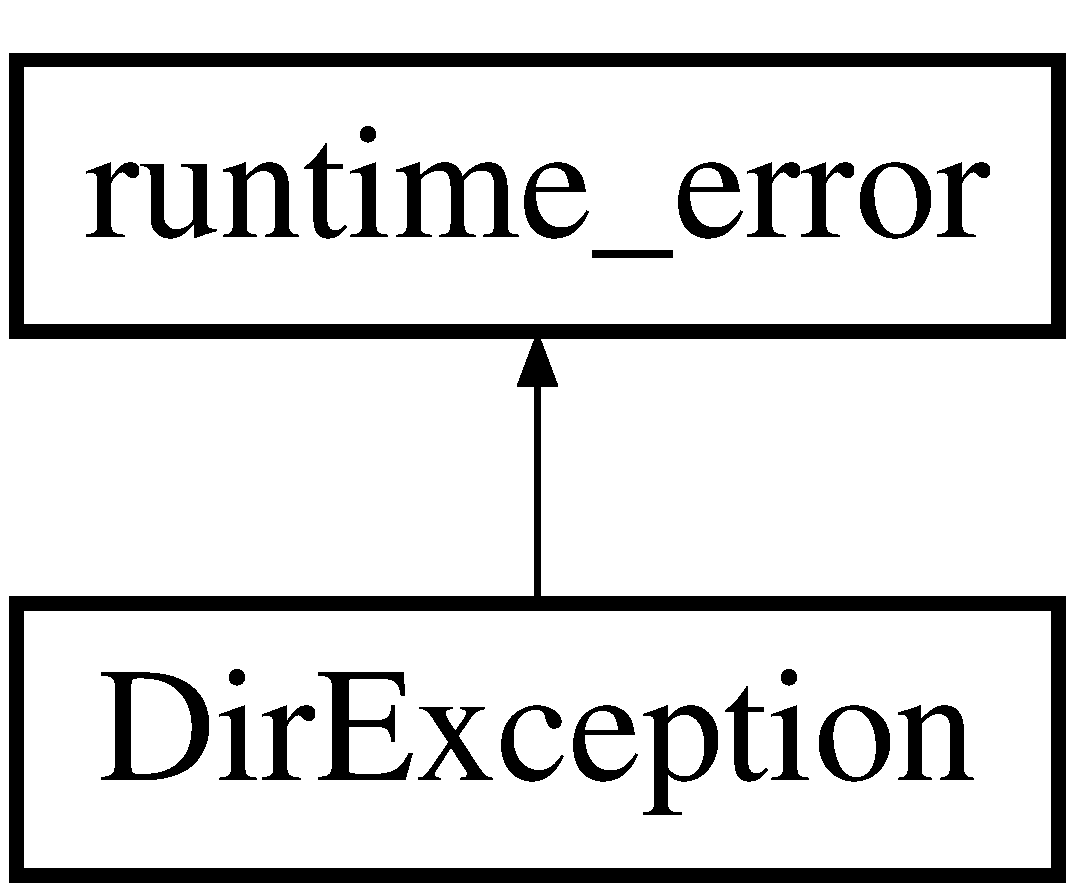
\includegraphics[height=2.000000cm]{classDirException}
\end{center}
\end{figure}
\subsection*{Public Member Functions}
\begin{DoxyCompactItemize}
\item 
{\bfseries Dir\+Exception} (const std\+::string \&message)\label{classDirException_a33ced612aa6ea89e5cc843e20d5c54c3}

\end{DoxyCompactItemize}


\subsection{Detailed Description}
This exception should be thrown when it is not possible create a directory. 

The documentation for this class was generated from the following file\+:\begin{DoxyCompactItemize}
\item 
/home/felipe/\+Desktop/vdsproject/vdscp\+\_\+04/src/bench/circuit\+\_\+to\+\_\+\+B\+D\+D\+\_\+manager.\+hpp\end{DoxyCompactItemize}

\section{Class\+Project\+:\+:Dot\+Bdd\+Dumper Class Reference}
\label{classClassProject_1_1DotBddDumper}\index{Class\+Project\+::\+Dot\+Bdd\+Dumper@{Class\+Project\+::\+Dot\+Bdd\+Dumper}}
Inheritance diagram for Class\+Project\+:\+:Dot\+Bdd\+Dumper\+:\begin{figure}[H]
\begin{center}
\leavevmode
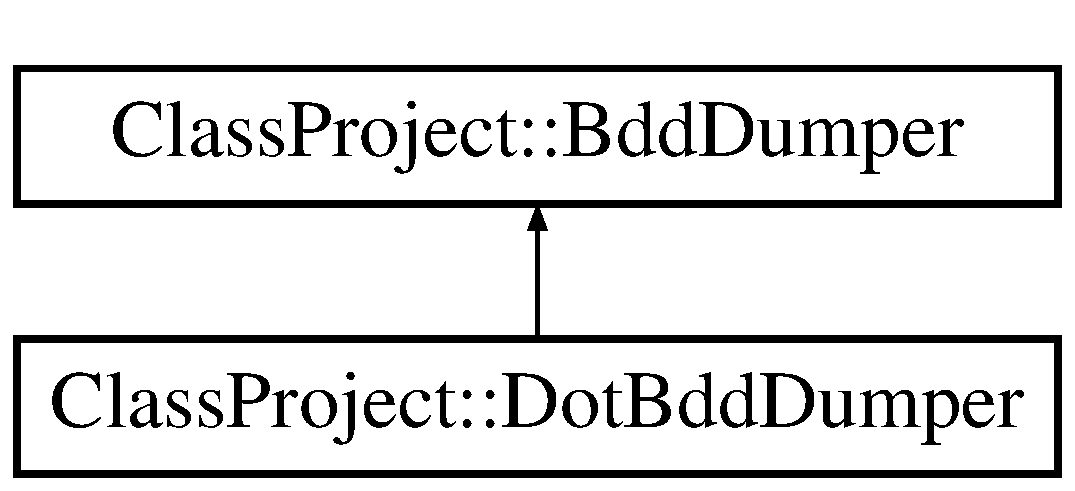
\includegraphics[height=2.000000cm]{classClassProject_1_1DotBddDumper}
\end{center}
\end{figure}
\subsection*{Public Member Functions}
\begin{DoxyCompactItemize}
\item 
{\bfseries Dot\+Bdd\+Dumper} ({\bf Manager} \&mgr)\label{classClassProject_1_1DotBddDumper_ae6ea6f970ccdff61558df2e2d5d71591}

\item 
virtual void {\bfseries dump} (const B\+D\+D\+\_\+\+ID \&root, std\+::ostream \&out)\label{classClassProject_1_1DotBddDumper_abcef13e93836b3827e1903a6ad6bed00}

\end{DoxyCompactItemize}


The documentation for this class was generated from the following files\+:\begin{DoxyCompactItemize}
\item 
/import/home/vdscp04/\+Luiz/vdscp\+\_\+04/src/bench/Dumper.\+h\item 
/import/home/vdscp04/\+Luiz/vdscp\+\_\+04/src/bench/Dumper.\+cpp\end{DoxyCompactItemize}

\section{ska\+:\+:detailv3\+:\+:Entry\+Default\+Table$<$ T $>$ Struct Template Reference}
\label{structska_1_1detailv3_1_1EntryDefaultTable}\index{ska\+::detailv3\+::\+Entry\+Default\+Table$<$ T $>$@{ska\+::detailv3\+::\+Entry\+Default\+Table$<$ T $>$}}
\subsection*{Static Public Attributes}
\begin{DoxyCompactItemize}
\item 
static constexpr const {\bf sherwood\+\_\+v3\+\_\+entry\+\_\+constexpr}$<$ T $>$ {\bfseries table} [min\+\_\+lookups]
\end{DoxyCompactItemize}


\subsection{Member Data Documentation}
\index{ska\+::detailv3\+::\+Entry\+Default\+Table@{ska\+::detailv3\+::\+Entry\+Default\+Table}!table@{table}}
\index{table@{table}!ska\+::detailv3\+::\+Entry\+Default\+Table@{ska\+::detailv3\+::\+Entry\+Default\+Table}}
\subsubsection[{table}]{\setlength{\rightskip}{0pt plus 5cm}template$<$typename T $>$ constexpr const {\bf sherwood\+\_\+v3\+\_\+entry\+\_\+constexpr}$<$ T $>$ {\bf ska\+::detailv3\+::\+Entry\+Default\+Table}$<$ T $>$\+::table\hspace{0.3cm}{\ttfamily [static]}}\label{structska_1_1detailv3_1_1EntryDefaultTable_a370614f6441cfac24df1f0f90102c8e5}
{\bfseries Initial value\+:}
\begin{DoxyCode}
=
    \{
        \{\}, \{\}, \{\}, sherwood\_v3\_entry\_constexpr<T>::special\_end\_entry()
    \}
\end{DoxyCode}


The documentation for this struct was generated from the following file\+:\begin{DoxyCompactItemize}
\item 
/home/felipe/\+Desktop/vdsproject/vdscp\+\_\+04/src/flat\+\_\+hash\+\_\+map.\+hpp\end{DoxyCompactItemize}

\section{File\+Exception Class Reference}
\label{classFileException}\index{File\+Exception@{File\+Exception}}


This exception should be thrown when it is not possible open a log file.  




{\ttfamily \#include $<$circuit\+\_\+to\+\_\+\+B\+D\+D\+\_\+manager.\+hpp$>$}

Inheritance diagram for File\+Exception\+:\begin{figure}[H]
\begin{center}
\leavevmode
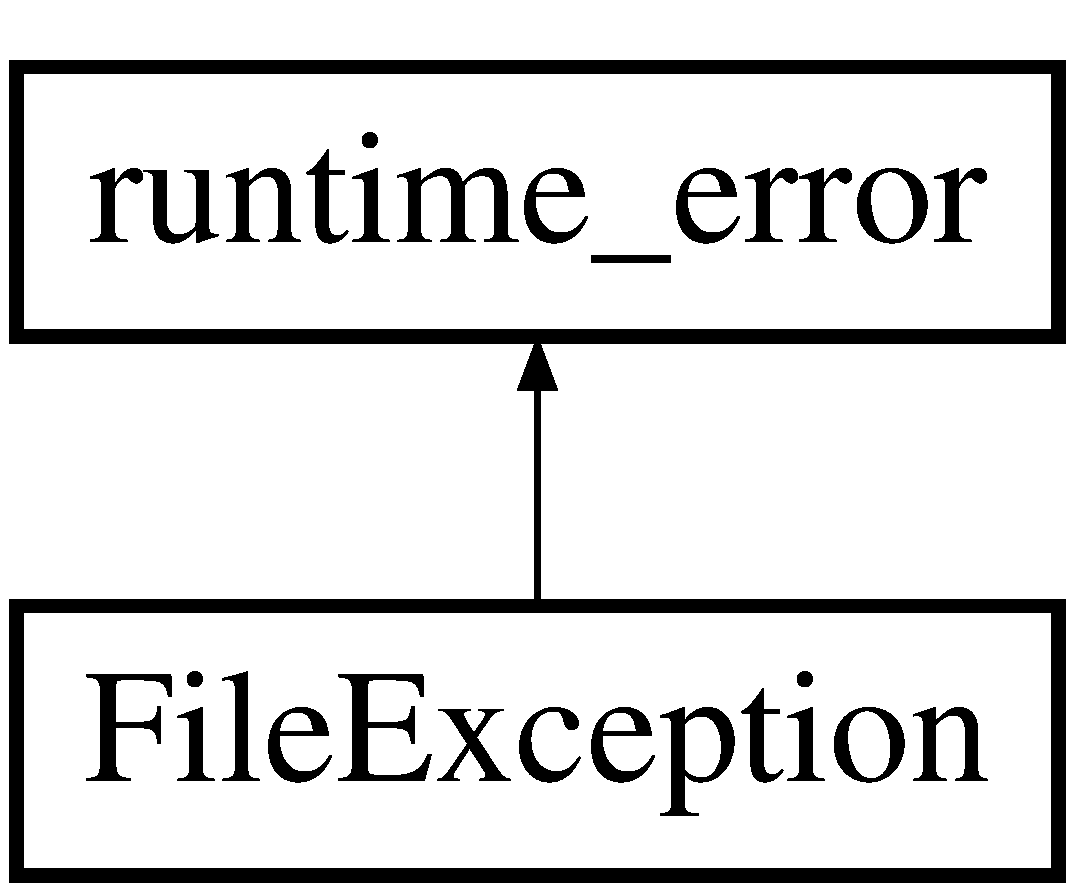
\includegraphics[height=2.000000cm]{classFileException}
\end{center}
\end{figure}
\subsection*{Public Member Functions}
\begin{DoxyCompactItemize}
\item 
{\bfseries File\+Exception} (const std\+::string \&message)\label{classFileException_a0d1f9f85f7fd4b70c619f80602ad1146}

\end{DoxyCompactItemize}


\subsection{Detailed Description}
This exception should be thrown when it is not possible open a log file. 

The documentation for this class was generated from the following file\+:\begin{DoxyCompactItemize}
\item 
/import/home/vdscp04/\+Luiz/vdscp\+\_\+04/src/bench/circuit\+\_\+to\+\_\+\+B\+D\+D\+\_\+manager.\+hpp\end{DoxyCompactItemize}

\section{ska\+:\+:flat\+\_\+hash\+\_\+map$<$ K, V, H, E, A $>$ Class Template Reference}
\label{classska_1_1flat__hash__map}\index{ska\+::flat\+\_\+hash\+\_\+map$<$ K, V, H, E, A $>$@{ska\+::flat\+\_\+hash\+\_\+map$<$ K, V, H, E, A $>$}}
Inheritance diagram for ska\+:\+:flat\+\_\+hash\+\_\+map$<$ K, V, H, E, A $>$\+:\begin{figure}[H]
\begin{center}
\leavevmode
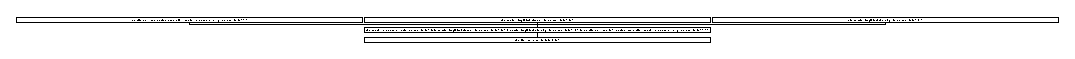
\includegraphics[height=0.345893cm]{classska_1_1flat__hash__map}
\end{center}
\end{figure}
\subsection*{Classes}
\begin{DoxyCompactItemize}
\item 
struct {\bf convertible\+\_\+to\+\_\+value}
\end{DoxyCompactItemize}
\subsection*{Public Types}
\begin{DoxyCompactItemize}
\item 
using {\bfseries key\+\_\+type} = K\label{classska_1_1flat__hash__map_ab22f477e2dfc6e682ee147fcf805e4a9}

\item 
using {\bfseries mapped\+\_\+type} = V\label{classska_1_1flat__hash__map_a1cb3116c3119b43080e0acdfde9a5ddd}

\end{DoxyCompactItemize}
\subsection*{Public Member Functions}
\begin{DoxyCompactItemize}
\item 
V \& {\bfseries operator[$\,$]} (const K \&key)\label{classska_1_1flat__hash__map_ada5db818bc094fba7e76006eeadf4ee9}

\item 
V \& {\bfseries operator[$\,$]} (K \&\&key)\label{classska_1_1flat__hash__map_a0585139dbbb10cf41b68d3968dbf2010}

\item 
V \& {\bfseries at} (const K \&key)\label{classska_1_1flat__hash__map_a374735760ecc82651cbb508a1d8866c1}

\item 
const V \& {\bfseries at} (const K \&key) const \label{classska_1_1flat__hash__map_a6facd6586c9856cbc577368cdb319ff3}

\item 
std\+::pair$<$ typename {\bf Table\+::iterator}, bool $>$ {\bfseries emplace} ()\label{classska_1_1flat__hash__map_a95175e5ecd48bbdb2d7820b833cefbb4}

\end{DoxyCompactItemize}
\subsection*{Private Types}
\begin{DoxyCompactItemize}
\item 
using {\bfseries Table} = {\bf detailv3\+::sherwood\+\_\+v3\+\_\+table}$<$ std\+::pair$<$ K, V $>$, K, H, {\bf detailv3\+::\+Key\+Or\+Value\+Hasher}$<$ K, std\+::pair$<$ K, V $>$, H $>$, E, {\bf detailv3\+::\+Key\+Or\+Value\+Equality}$<$ K, std\+::pair$<$ K, V $>$, E $>$, A, typename std\+::allocator\+\_\+traits$<$ A $>$\+::template rebind\+\_\+alloc$<$ {\bf detailv3\+::sherwood\+\_\+v3\+\_\+entry}$<$ std\+::pair$<$ K, V $>$$>$$>$ $>$\label{classska_1_1flat__hash__map_a6ef9f5f58e71eae864a3cc89d29e0c4b}

\end{DoxyCompactItemize}
\subsection*{Friends}
\begin{DoxyCompactItemize}
\item 
bool {\bfseries operator==} (const {\bf flat\+\_\+hash\+\_\+map} \&lhs, const {\bf flat\+\_\+hash\+\_\+map} \&rhs)\label{classska_1_1flat__hash__map_a469dfb7c5084c0ebd754590f1e78ae87}

\item 
bool {\bfseries operator!=} (const {\bf flat\+\_\+hash\+\_\+map} \&lhs, const {\bf flat\+\_\+hash\+\_\+map} \&rhs)\label{classska_1_1flat__hash__map_a62328dcbb77072758a4f1f68db6f5e2a}

\end{DoxyCompactItemize}


The documentation for this class was generated from the following file\+:\begin{DoxyCompactItemize}
\item 
/home/felipe/\+Desktop/vdsproject/vdscp\+\_\+04/src/flat\+\_\+hash\+\_\+map.\+hpp\end{DoxyCompactItemize}

\section{ska\+:\+:flat\+\_\+hash\+\_\+set$<$ T, H, E, A $>$ Class Template Reference}
\label{classska_1_1flat__hash__set}\index{ska\+::flat\+\_\+hash\+\_\+set$<$ T, H, E, A $>$@{ska\+::flat\+\_\+hash\+\_\+set$<$ T, H, E, A $>$}}
Inheritance diagram for ska\+:\+:flat\+\_\+hash\+\_\+set$<$ T, H, E, A $>$\+:\begin{figure}[H]
\begin{center}
\leavevmode
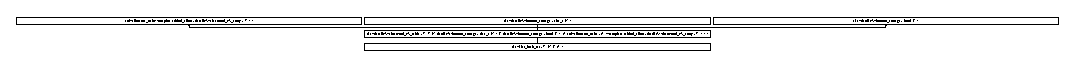
\includegraphics[height=0.454915cm]{classska_1_1flat__hash__set}
\end{center}
\end{figure}
\subsection*{Public Types}
\begin{DoxyCompactItemize}
\item 
using {\bfseries key\+\_\+type} = T\label{classska_1_1flat__hash__set_a2e9fb96bdde61d77d3a05f4457e96289}

\end{DoxyCompactItemize}
\subsection*{Public Member Functions}
\begin{DoxyCompactItemize}
\item 
{\footnotesize template$<$typename... Args$>$ }\\std\+::pair$<$ typename {\bf Table\+::iterator}, bool $>$ {\bfseries emplace} (Args \&\&...args)\label{classska_1_1flat__hash__set_ad92ec1589a6548f38756badd324f9e82}

\item 
std\+::pair$<$ typename {\bf Table\+::iterator}, bool $>$ {\bfseries emplace} (const key\+\_\+type \&arg)\label{classska_1_1flat__hash__set_aa93b866342936f757aa1b9ac4846886f}

\item 
std\+::pair$<$ typename {\bf Table\+::iterator}, bool $>$ {\bfseries emplace} (key\+\_\+type \&arg)\label{classska_1_1flat__hash__set_a8ba97bef14dbc916412381ca6fbb469f}

\item 
std\+::pair$<$ typename {\bf Table\+::iterator}, bool $>$ {\bfseries emplace} (const key\+\_\+type \&\&arg)\label{classska_1_1flat__hash__set_a48673c1c502f55811391ae15c700269a}

\item 
std\+::pair$<$ typename {\bf Table\+::iterator}, bool $>$ {\bfseries emplace} (key\+\_\+type \&\&arg)\label{classska_1_1flat__hash__set_a22a0114b463d2c3b598bf367e5266c92}

\end{DoxyCompactItemize}
\subsection*{Private Types}
\begin{DoxyCompactItemize}
\item 
using {\bfseries Table} = {\bf detailv3\+::sherwood\+\_\+v3\+\_\+table}$<$ T, T, H, {\bf detailv3\+::functor\+\_\+storage}$<$ size\+\_\+t, H $>$, E, {\bf detailv3\+::functor\+\_\+storage}$<$ bool, E $>$, A, typename std\+::allocator\+\_\+traits$<$ A $>$\+::template rebind\+\_\+alloc$<$ {\bf detailv3\+::sherwood\+\_\+v3\+\_\+entry}$<$ T $>$$>$ $>$\label{classska_1_1flat__hash__set_a737da60f812c6fc7ee564d692c7ec0ec}

\end{DoxyCompactItemize}
\subsection*{Friends}
\begin{DoxyCompactItemize}
\item 
bool {\bfseries operator==} (const {\bf flat\+\_\+hash\+\_\+set} \&lhs, const {\bf flat\+\_\+hash\+\_\+set} \&rhs)\label{classska_1_1flat__hash__set_a983dec7661d28492024dc5f4fc5c05d9}

\item 
bool {\bfseries operator!=} (const {\bf flat\+\_\+hash\+\_\+set} \&lhs, const {\bf flat\+\_\+hash\+\_\+set} \&rhs)\label{classska_1_1flat__hash__set_a978a1892e7a55293cc37ad445d7e9978}

\end{DoxyCompactItemize}


The documentation for this class was generated from the following file\+:\begin{DoxyCompactItemize}
\item 
/home/felipe/\+Desktop/vdsproject/vdscp\+\_\+04/src/flat\+\_\+hash\+\_\+map.\+hpp\end{DoxyCompactItemize}

\section{ska\+:\+:detailv3\+:\+:functor\+\_\+storage$<$ Result, Functor $>$ Struct Template Reference}
\label{structska_1_1detailv3_1_1functor__storage}\index{ska\+::detailv3\+::functor\+\_\+storage$<$ Result, Functor $>$@{ska\+::detailv3\+::functor\+\_\+storage$<$ Result, Functor $>$}}
Inheritance diagram for ska\+:\+:detailv3\+:\+:functor\+\_\+storage$<$ Result, Functor $>$\+:\begin{figure}[H]
\begin{center}
\leavevmode
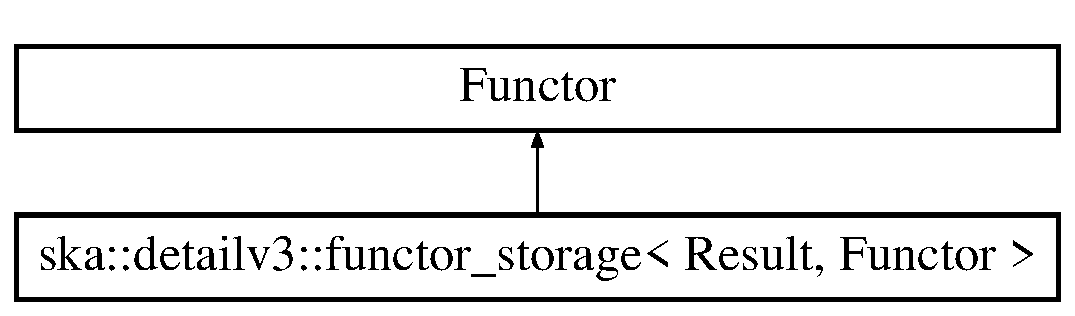
\includegraphics[height=2.000000cm]{structska_1_1detailv3_1_1functor__storage}
\end{center}
\end{figure}
\subsection*{Public Member Functions}
\begin{DoxyCompactItemize}
\item 
{\bfseries functor\+\_\+storage} (const Functor \&functor)\label{structska_1_1detailv3_1_1functor__storage_a5e4eb7609b4baf949e46c598e255e2d2}

\item 
{\footnotesize template$<$typename... Args$>$ }\\Result {\bfseries operator()} (Args \&\&...args)\label{structska_1_1detailv3_1_1functor__storage_a024a67f954462da36d97466dacfe9128}

\item 
{\footnotesize template$<$typename... Args$>$ }\\Result {\bfseries operator()} (Args \&\&...args) const \label{structska_1_1detailv3_1_1functor__storage_a3bbebb63a713a5eedd4acb3d55f6ffc4}

\end{DoxyCompactItemize}


The documentation for this struct was generated from the following file\+:\begin{DoxyCompactItemize}
\item 
/home/felipe/\+Desktop/vdsproject/vdscp\+\_\+04/src/flat\+\_\+hash\+\_\+map.\+hpp\end{DoxyCompactItemize}

\section{ska\+:\+:detailv3\+:\+:functor\+\_\+storage$<$ Result, Result($\ast$)(Args...)$>$ Struct Template Reference}
\label{structska_1_1detailv3_1_1functor__storage_3_01Result_00_01Result_07_5_08_07Args_8_8_8_08_4}\index{ska\+::detailv3\+::functor\+\_\+storage$<$ Result, Result($\ast$)(\+Args...)$>$@{ska\+::detailv3\+::functor\+\_\+storage$<$ Result, Result($\ast$)(\+Args...)$>$}}
\subsection*{Public Types}
\begin{DoxyCompactItemize}
\item 
typedef Result($\ast$ {\bfseries function\+\_\+ptr}) (Args...)\label{structska_1_1detailv3_1_1functor__storage_3_01Result_00_01Result_07_5_08_07Args_8_8_8_08_4_a59181fac378d8220ef1cdb364d8cbc52}

\end{DoxyCompactItemize}
\subsection*{Public Member Functions}
\begin{DoxyCompactItemize}
\item 
{\bfseries functor\+\_\+storage} (function\+\_\+ptr function)\label{structska_1_1detailv3_1_1functor__storage_3_01Result_00_01Result_07_5_08_07Args_8_8_8_08_4_a975cd58296e05a0e1c231de3c34dfe01}

\item 
Result {\bfseries operator()} (Args...\+args) const \label{structska_1_1detailv3_1_1functor__storage_3_01Result_00_01Result_07_5_08_07Args_8_8_8_08_4_af76a0835878cf61fe98690df661f5b79}

\item 
{\bfseries operator function\+\_\+ptr \&} ()\label{structska_1_1detailv3_1_1functor__storage_3_01Result_00_01Result_07_5_08_07Args_8_8_8_08_4_a5fff6851ad46ba4b32856030d6ee8e31}

\item 
{\bfseries operator const function\+\_\+ptr \&} ()\label{structska_1_1detailv3_1_1functor__storage_3_01Result_00_01Result_07_5_08_07Args_8_8_8_08_4_abdf5e725c6a6b3c1f09ca3385fa7c553}

\end{DoxyCompactItemize}
\subsection*{Public Attributes}
\begin{DoxyCompactItemize}
\item 
function\+\_\+ptr {\bfseries function}\label{structska_1_1detailv3_1_1functor__storage_3_01Result_00_01Result_07_5_08_07Args_8_8_8_08_4_a84b9752fc57d45de4111134a580b72c1}

\end{DoxyCompactItemize}


The documentation for this struct was generated from the following file\+:\begin{DoxyCompactItemize}
\item 
/home/felipe/\+Desktop/vdsproject/vdscp\+\_\+04/src/flat\+\_\+hash\+\_\+map.\+hpp\end{DoxyCompactItemize}

\section{std\+:\+:hash$<$ boost\+:\+:uuids\+:\+:uuid $>$ Struct Template Reference}
\label{structstd_1_1hash_3_01boost_1_1uuids_1_1uuid_01_4}\index{std\+::hash$<$ boost\+::uuids\+::uuid $>$@{std\+::hash$<$ boost\+::uuids\+::uuid $>$}}
\subsection*{Public Member Functions}
\begin{DoxyCompactItemize}
\item 
size\+\_\+t {\bfseries operator()} (const boost\+::uuids\+::uuid \&uid)\label{structstd_1_1hash_3_01boost_1_1uuids_1_1uuid_01_4_a6ac7c463e75133c7febbd66f13a9c1dc}

\end{DoxyCompactItemize}


The documentation for this struct was generated from the following file\+:\begin{DoxyCompactItemize}
\item 
/import/home/vdscp04/\+Luiz/vdscp\+\_\+04/src/bench/bench\+\_\+circuit\+\_\+manager.\+hpp\end{DoxyCompactItemize}

\section{ska\+:\+:detailv3\+:\+:Hash\+Policy\+Selector$<$ T, typename $>$ Struct Template Reference}
\label{structska_1_1detailv3_1_1HashPolicySelector}\index{ska\+::detailv3\+::\+Hash\+Policy\+Selector$<$ T, typename $>$@{ska\+::detailv3\+::\+Hash\+Policy\+Selector$<$ T, typename $>$}}
\subsection*{Public Types}
\begin{DoxyCompactItemize}
\item 
typedef {\bf prime\+\_\+number\+\_\+hash\+\_\+policy} {\bfseries type}\label{structska_1_1detailv3_1_1HashPolicySelector_a49f01419b9072972f37c66571456957a}

\end{DoxyCompactItemize}


The documentation for this struct was generated from the following file\+:\begin{DoxyCompactItemize}
\item 
/home/felipe/\+Desktop/vdsproject/vdscp\+\_\+04/src/flat\+\_\+hash\+\_\+map.\+hpp\end{DoxyCompactItemize}

\section{ska\+:\+:detailv3\+:\+:Hash\+Policy\+Selector$<$ T, void\+\_\+t$<$ typename T\+:\+:hash\+\_\+policy $>$ $>$ Struct Template Reference}
\label{structska_1_1detailv3_1_1HashPolicySelector_3_01T_00_01void__t_3_01typename_01T_1_1hash__policy_01_4_01_4}\index{ska\+::detailv3\+::\+Hash\+Policy\+Selector$<$ T, void\+\_\+t$<$ typename T\+::hash\+\_\+policy $>$ $>$@{ska\+::detailv3\+::\+Hash\+Policy\+Selector$<$ T, void\+\_\+t$<$ typename T\+::hash\+\_\+policy $>$ $>$}}
\subsection*{Public Types}
\begin{DoxyCompactItemize}
\item 
typedef T\+::hash\+\_\+policy {\bfseries type}\label{structska_1_1detailv3_1_1HashPolicySelector_3_01T_00_01void__t_3_01typename_01T_1_1hash__policy_01_4_01_4_a7d2e238bd61f99a9749a749fe06b795c}

\end{DoxyCompactItemize}


The documentation for this struct was generated from the following file\+:\begin{DoxyCompactItemize}
\item 
/home/felipe/\+Desktop/vdsproject/vdscp\+\_\+04/src/flat\+\_\+hash\+\_\+map.\+hpp\end{DoxyCompactItemize}

\section{Inexistent\+B\+D\+D\+\_\+\+I\+D\+Exception Class Reference}
\label{classInexistentBDD__IDException}\index{Inexistent\+B\+D\+D\+\_\+\+I\+D\+Exception@{Inexistent\+B\+D\+D\+\_\+\+I\+D\+Exception}}


This exception should be thrown when an invalid B\+D\+D\+\_\+\+ID is passed as parameter.  




{\ttfamily \#include $<$circuit\+\_\+to\+\_\+\+B\+D\+D\+\_\+manager.\+hpp$>$}

Inheritance diagram for Inexistent\+B\+D\+D\+\_\+\+I\+D\+Exception\+:\begin{figure}[H]
\begin{center}
\leavevmode
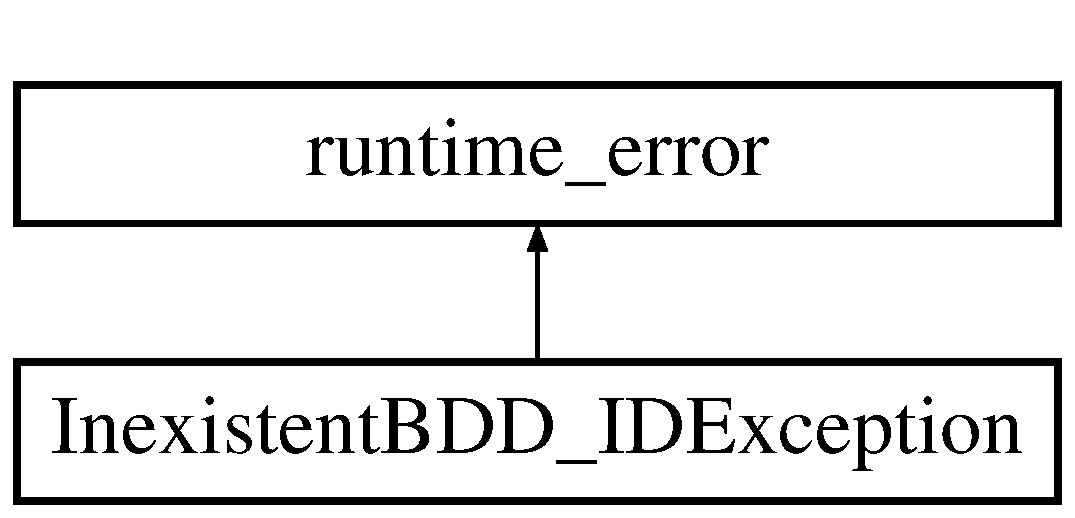
\includegraphics[height=2.000000cm]{classInexistentBDD__IDException}
\end{center}
\end{figure}
\subsection*{Public Member Functions}
\begin{DoxyCompactItemize}
\item 
{\bfseries Inexistent\+B\+D\+D\+\_\+\+I\+D\+Exception} (const std\+::string \&message)\label{classInexistentBDD__IDException_a574d927fc98d356d1ff18cef3d32ffb5}

\end{DoxyCompactItemize}


\subsection{Detailed Description}
This exception should be thrown when an invalid B\+D\+D\+\_\+\+ID is passed as parameter. 

The documentation for this class was generated from the following file\+:\begin{DoxyCompactItemize}
\item 
/import/home/vdscp04/\+Luiz/vdscp\+\_\+04/src/bench/circuit\+\_\+to\+\_\+\+B\+D\+D\+\_\+manager.\+hpp\end{DoxyCompactItemize}

\section{Inexistent\+B\+D\+D\+Label\+Exception Class Reference}
\label{classInexistentBDDLabelException}\index{Inexistent\+B\+D\+D\+Label\+Exception@{Inexistent\+B\+D\+D\+Label\+Exception}}


This exception should be thrown when an Inexistent label is called.  




{\ttfamily \#include $<$circuit\+\_\+to\+\_\+\+B\+D\+D\+\_\+manager.\+hpp$>$}

Inheritance diagram for Inexistent\+B\+D\+D\+Label\+Exception\+:\begin{figure}[H]
\begin{center}
\leavevmode
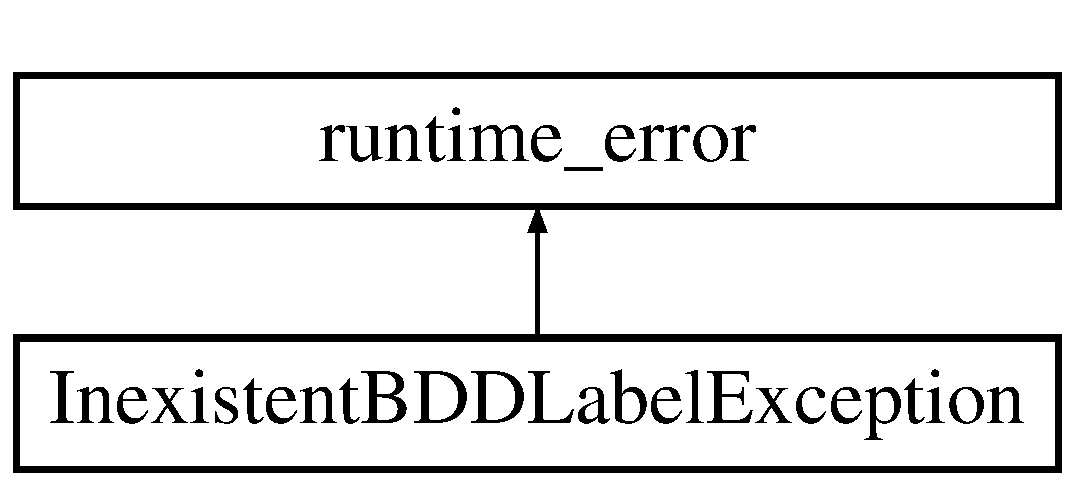
\includegraphics[height=2.000000cm]{classInexistentBDDLabelException}
\end{center}
\end{figure}
\subsection*{Public Member Functions}
\begin{DoxyCompactItemize}
\item 
{\bfseries Inexistent\+B\+D\+D\+Label\+Exception} (const std\+::string \&message)\label{classInexistentBDDLabelException_a04979bc3d74b3d2ec7b0232639b9c862}

\end{DoxyCompactItemize}


\subsection{Detailed Description}
This exception should be thrown when an Inexistent label is called. 

The documentation for this class was generated from the following file\+:\begin{DoxyCompactItemize}
\item 
/import/home/vdscp04/\+Luiz/vdscp\+\_\+04/src/bench/circuit\+\_\+to\+\_\+\+B\+D\+D\+\_\+manager.\+hpp\end{DoxyCompactItemize}

\section{Inexistent\+Label\+Exception Class Reference}
\label{classInexistentLabelException}\index{Inexistent\+Label\+Exception@{Inexistent\+Label\+Exception}}


This exception should be thrown when an invalid label\+\_\+t is passed as parameter.  




{\ttfamily \#include $<$bench\+\_\+circuit\+\_\+manager.\+hpp$>$}

Inheritance diagram for Inexistent\+Label\+Exception\+:\begin{figure}[H]
\begin{center}
\leavevmode
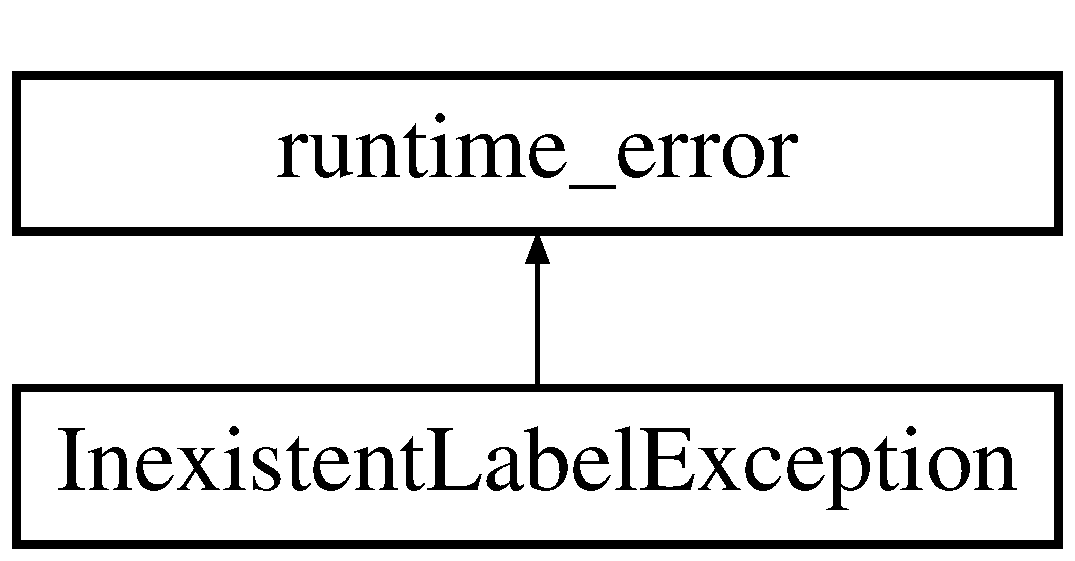
\includegraphics[height=2.000000cm]{classInexistentLabelException}
\end{center}
\end{figure}
\subsection*{Public Member Functions}
\begin{DoxyCompactItemize}
\item 
{\bfseries Inexistent\+Label\+Exception} (const std\+::string \&message)\label{classInexistentLabelException_a10aad583eea5fb78eb56695b80a8da27}

\end{DoxyCompactItemize}


\subsection{Detailed Description}
This exception should be thrown when an invalid label\+\_\+t is passed as parameter. 

The documentation for this class was generated from the following file\+:\begin{DoxyCompactItemize}
\item 
/home/felipe/\+Desktop/vdsproject/vdscp\+\_\+04/src/bench/bench\+\_\+circuit\+\_\+manager.\+hpp\end{DoxyCompactItemize}

\section{Inexistent\+U\+U\+I\+D\+Exception Class Reference}
\label{classInexistentUUIDException}\index{Inexistent\+U\+U\+I\+D\+Exception@{Inexistent\+U\+U\+I\+D\+Exception}}


This exception should be thrown when an invalid unique\+\_\+\+I\+D\+\_\+t is passed as parameter.  




{\ttfamily \#include $<$bench\+\_\+circuit\+\_\+manager.\+hpp$>$}

Inheritance diagram for Inexistent\+U\+U\+I\+D\+Exception\+:\begin{figure}[H]
\begin{center}
\leavevmode
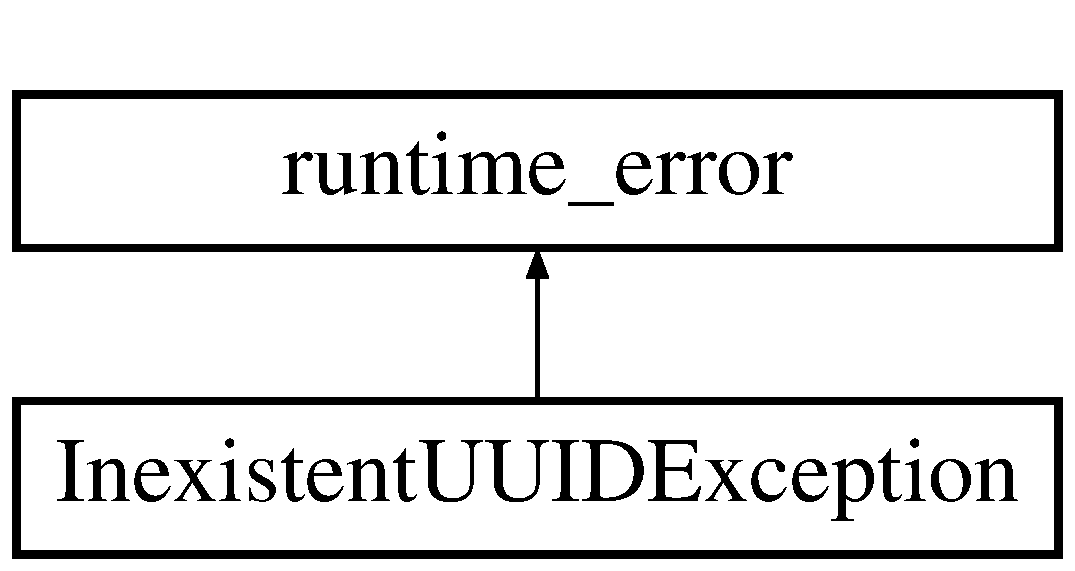
\includegraphics[height=2.000000cm]{classInexistentUUIDException}
\end{center}
\end{figure}
\subsection*{Public Member Functions}
\begin{DoxyCompactItemize}
\item 
{\bfseries Inexistent\+U\+U\+I\+D\+Exception} (const std\+::string \&message)\label{classInexistentUUIDException_a3a63e43f2b5d726f2cb99a90ff382cbf}

\end{DoxyCompactItemize}


\subsection{Detailed Description}
This exception should be thrown when an invalid unique\+\_\+\+I\+D\+\_\+t is passed as parameter. 

The documentation for this class was generated from the following file\+:\begin{DoxyCompactItemize}
\item 
/home/felipe/\+Desktop/vdsproject/vdscp\+\_\+04/src/bench/bench\+\_\+circuit\+\_\+manager.\+hpp\end{DoxyCompactItemize}

\section{ska\+:\+:detailv3\+:\+:Key\+Or\+Value\+Equality$<$ key\+\_\+type, value\+\_\+type, key\+\_\+equal $>$ Struct Template Reference}
\label{structska_1_1detailv3_1_1KeyOrValueEquality}\index{ska\+::detailv3\+::\+Key\+Or\+Value\+Equality$<$ key\+\_\+type, value\+\_\+type, key\+\_\+equal $>$@{ska\+::detailv3\+::\+Key\+Or\+Value\+Equality$<$ key\+\_\+type, value\+\_\+type, key\+\_\+equal $>$}}
Inheritance diagram for ska\+:\+:detailv3\+:\+:Key\+Or\+Value\+Equality$<$ key\+\_\+type, value\+\_\+type, key\+\_\+equal $>$\+:\begin{figure}[H]
\begin{center}
\leavevmode
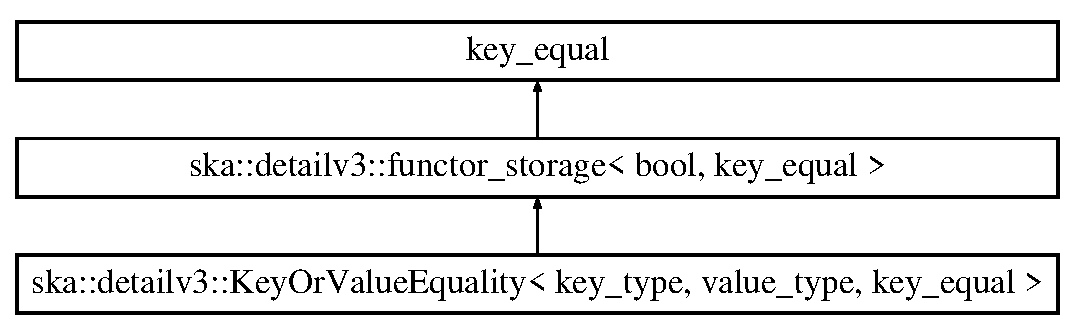
\includegraphics[height=3.000000cm]{structska_1_1detailv3_1_1KeyOrValueEquality}
\end{center}
\end{figure}
\subsection*{Public Types}
\begin{DoxyCompactItemize}
\item 
typedef {\bf functor\+\_\+storage}$<$ bool, key\+\_\+equal $>$ {\bfseries equality\+\_\+storage}\label{structska_1_1detailv3_1_1KeyOrValueEquality_ada804457efc64bb51a705877f6b029d3}

\end{DoxyCompactItemize}
\subsection*{Public Member Functions}
\begin{DoxyCompactItemize}
\item 
{\bfseries Key\+Or\+Value\+Equality} (const key\+\_\+equal \&equality)\label{structska_1_1detailv3_1_1KeyOrValueEquality_ae01de1db32c5e78bb02eb2a4b39038d6}

\item 
bool {\bfseries operator()} (const key\+\_\+type \&lhs, const key\+\_\+type \&rhs)\label{structska_1_1detailv3_1_1KeyOrValueEquality_a1f49bb215f288d746d81bd7c13f4e1a3}

\item 
bool {\bfseries operator()} (const key\+\_\+type \&lhs, const value\+\_\+type \&rhs)\label{structska_1_1detailv3_1_1KeyOrValueEquality_a976fa386f1387dde3457f0c67f1034b9}

\item 
bool {\bfseries operator()} (const value\+\_\+type \&lhs, const key\+\_\+type \&rhs)\label{structska_1_1detailv3_1_1KeyOrValueEquality_a209e09a271461a963b34eb0a75da6fcf}

\item 
bool {\bfseries operator()} (const value\+\_\+type \&lhs, const value\+\_\+type \&rhs)\label{structska_1_1detailv3_1_1KeyOrValueEquality_a0df018fa35a9d286e05dbab4ada0c113}

\item 
{\footnotesize template$<$typename F , typename S $>$ }\\bool {\bfseries operator()} (const key\+\_\+type \&lhs, const std\+::pair$<$ F, S $>$ \&rhs)\label{structska_1_1detailv3_1_1KeyOrValueEquality_a3f650d3490f8b2e6b775f972bdeaecc2}

\item 
{\footnotesize template$<$typename F , typename S $>$ }\\bool {\bfseries operator()} (const std\+::pair$<$ F, S $>$ \&lhs, const key\+\_\+type \&rhs)\label{structska_1_1detailv3_1_1KeyOrValueEquality_a7c47486d4150c2db2ad0b67dffde5523}

\item 
{\footnotesize template$<$typename F , typename S $>$ }\\bool {\bfseries operator()} (const value\+\_\+type \&lhs, const std\+::pair$<$ F, S $>$ \&rhs)\label{structska_1_1detailv3_1_1KeyOrValueEquality_ac4a05483fd81f73359f6a238dd58e735}

\item 
{\footnotesize template$<$typename F , typename S $>$ }\\bool {\bfseries operator()} (const std\+::pair$<$ F, S $>$ \&lhs, const value\+\_\+type \&rhs)\label{structska_1_1detailv3_1_1KeyOrValueEquality_aa7884496aa9d2e7d4dcdb96afc48a4ff}

\item 
{\footnotesize template$<$typename FL , typename SL , typename FR , typename SR $>$ }\\bool {\bfseries operator()} (const std\+::pair$<$ FL, SL $>$ \&lhs, const std\+::pair$<$ FR, SR $>$ \&rhs)\label{structska_1_1detailv3_1_1KeyOrValueEquality_a44362fa34b55c87e3f4e9b0d2906770b}

\end{DoxyCompactItemize}


The documentation for this struct was generated from the following file\+:\begin{DoxyCompactItemize}
\item 
/home/felipe/\+Desktop/vdsproject/vdscp\+\_\+04/src/flat\+\_\+hash\+\_\+map.\+hpp\end{DoxyCompactItemize}

\section{ska\+:\+:detailv3\+:\+:Key\+Or\+Value\+Hasher$<$ key\+\_\+type, value\+\_\+type, hasher $>$ Struct Template Reference}
\label{structska_1_1detailv3_1_1KeyOrValueHasher}\index{ska\+::detailv3\+::\+Key\+Or\+Value\+Hasher$<$ key\+\_\+type, value\+\_\+type, hasher $>$@{ska\+::detailv3\+::\+Key\+Or\+Value\+Hasher$<$ key\+\_\+type, value\+\_\+type, hasher $>$}}
Inheritance diagram for ska\+:\+:detailv3\+:\+:Key\+Or\+Value\+Hasher$<$ key\+\_\+type, value\+\_\+type, hasher $>$\+:\begin{figure}[H]
\begin{center}
\leavevmode
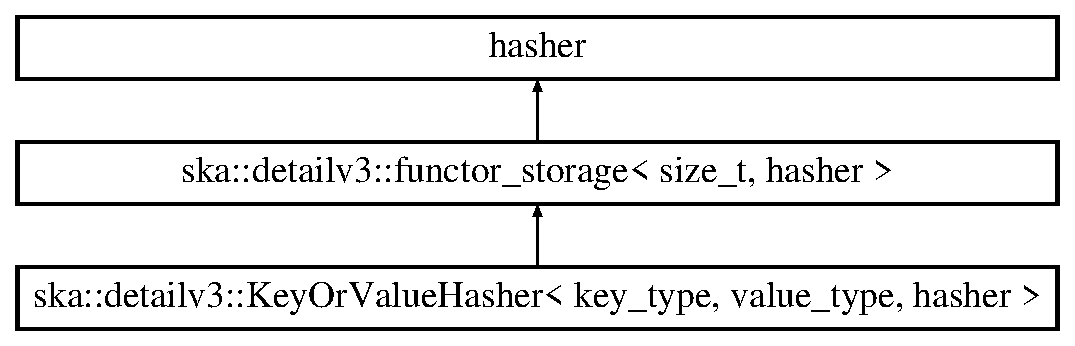
\includegraphics[height=3.000000cm]{structska_1_1detailv3_1_1KeyOrValueHasher}
\end{center}
\end{figure}
\subsection*{Public Types}
\begin{DoxyCompactItemize}
\item 
typedef {\bf functor\+\_\+storage}$<$ size\+\_\+t, hasher $>$ {\bfseries hasher\+\_\+storage}\label{structska_1_1detailv3_1_1KeyOrValueHasher_a1209a00d8459b8b5b476e66639738493}

\end{DoxyCompactItemize}
\subsection*{Public Member Functions}
\begin{DoxyCompactItemize}
\item 
{\bfseries Key\+Or\+Value\+Hasher} (const hasher \&hash)\label{structska_1_1detailv3_1_1KeyOrValueHasher_a4a39b08d7dae78f6d8a64e81edf6224d}

\item 
size\+\_\+t {\bfseries operator()} (const key\+\_\+type \&key)\label{structska_1_1detailv3_1_1KeyOrValueHasher_aa00b948e4a4e0c8ec76710b145a8d3f3}

\item 
size\+\_\+t {\bfseries operator()} (const key\+\_\+type \&key) const \label{structska_1_1detailv3_1_1KeyOrValueHasher_a0992593aec2cb1737e67380b4b2010fa}

\item 
size\+\_\+t {\bfseries operator()} (const value\+\_\+type \&value)\label{structska_1_1detailv3_1_1KeyOrValueHasher_a04c97c4e8eefda2592d030775bacfc5b}

\item 
size\+\_\+t {\bfseries operator()} (const value\+\_\+type \&value) const \label{structska_1_1detailv3_1_1KeyOrValueHasher_ae69dbe0f39291f853aa10fe75ec04875}

\item 
{\footnotesize template$<$typename F , typename S $>$ }\\size\+\_\+t {\bfseries operator()} (const std\+::pair$<$ F, S $>$ \&value)\label{structska_1_1detailv3_1_1KeyOrValueHasher_a5473ea70e3e1ab195c5cc092de851e28}

\item 
{\footnotesize template$<$typename F , typename S $>$ }\\size\+\_\+t {\bfseries operator()} (const std\+::pair$<$ F, S $>$ \&value) const \label{structska_1_1detailv3_1_1KeyOrValueHasher_adb3364a50047fa36d9b7904321f68155}

\end{DoxyCompactItemize}


The documentation for this struct was generated from the following file\+:\begin{DoxyCompactItemize}
\item 
/home/felipe/\+Desktop/vdsproject/vdscp\+\_\+04/src/flat\+\_\+hash\+\_\+map.\+hpp\end{DoxyCompactItemize}

\section{Class\+Project\+:\+:Manager Class Reference}
\label{classClassProject_1_1Manager}\index{Class\+Project\+::\+Manager@{Class\+Project\+::\+Manager}}


\doxyref{Manager}{p.}{classClassProject_1_1Manager} Class.  




{\ttfamily \#include $<$Manager.\+h$>$}

Inheritance diagram for Class\+Project\+:\+:Manager\+:\begin{figure}[H]
\begin{center}
\leavevmode
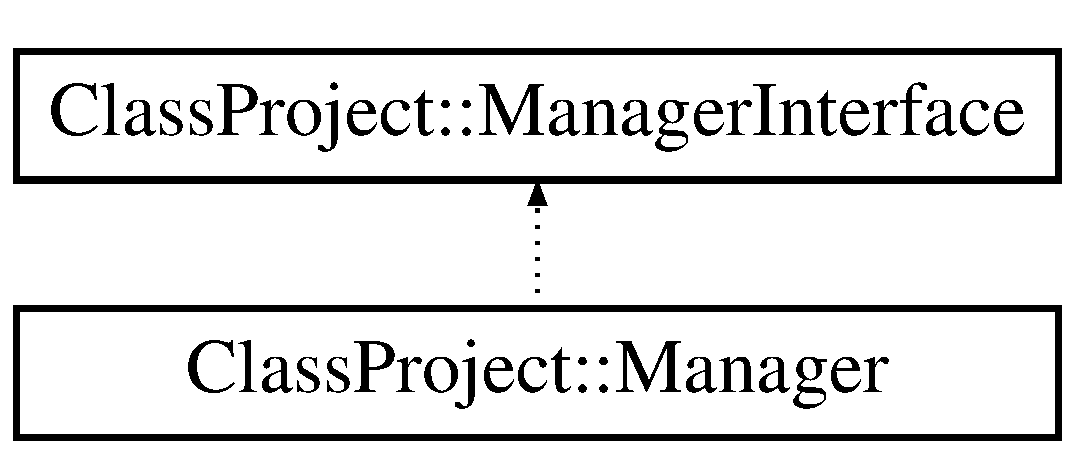
\includegraphics[height=2.000000cm]{classClassProject_1_1Manager}
\end{center}
\end{figure}
\subsection*{Public Member Functions}
\begin{DoxyCompactItemize}
\item 
{\bf Manager} ()
\begin{DoxyCompactList}\small\item\em \doxyref{Manager}{p.}{classClassProject_1_1Manager} Class. \end{DoxyCompactList}\item 
B\+D\+D\+\_\+\+ID {\bf create\+Var} (const std\+::string \&label) override
\begin{DoxyCompactList}\small\item\em Function to create a new Variable. \end{DoxyCompactList}\item 
const B\+D\+D\+\_\+\+ID \& {\bf True} () override
\begin{DoxyCompactList}\small\item\em Function to return the id of the T\+R\+UE leaf node in the Binary Tree. \end{DoxyCompactList}\item 
const B\+D\+D\+\_\+\+ID \& {\bf False} () override
\begin{DoxyCompactList}\small\item\em Function to return the id of the F\+A\+L\+SE leaf node in the Binary Tree. \end{DoxyCompactList}\item 
bool {\bf is\+Constant} (const B\+D\+D\+\_\+\+ID f) override
\begin{DoxyCompactList}\small\item\em Function to test if a given B\+D\+D\+\_\+\+ID is a Constant. \end{DoxyCompactList}\item 
bool {\bf is\+Variable} (const B\+D\+D\+\_\+\+ID x) override
\begin{DoxyCompactList}\small\item\em Function to test if a given B\+D\+D\+\_\+\+ID is a Variable. \end{DoxyCompactList}\item 
B\+D\+D\+\_\+\+ID {\bf top\+Var} (const B\+D\+D\+\_\+\+ID f) override
\begin{DoxyCompactList}\small\item\em Function to return the top variable of a given B\+D\+D\+\_\+\+ID. \end{DoxyCompactList}\item 
B\+D\+D\+\_\+\+ID {\bf ite} (const B\+D\+D\+\_\+\+ID i, const B\+D\+D\+\_\+\+ID t, const B\+D\+D\+\_\+\+ID e) override
\begin{DoxyCompactList}\small\item\em Function to compute the I\+F(\+B\+D\+D\+\_\+\+I\+D i) then(\+B\+D\+D\+\_\+\+I\+D t) E\+L\+S\+E(\+B\+D\+D\+\_\+\+I\+D e) Operator. \end{DoxyCompactList}\item 
B\+D\+D\+\_\+\+ID {\bf co\+Factor\+True} (const B\+D\+D\+\_\+\+ID f, B\+D\+D\+\_\+\+ID x) override
\begin{DoxyCompactList}\small\item\em Function to compute the T\+R\+UE co\+Factor of a given B\+D\+D\+\_\+\+ID f with respect to B\+D\+D\+\_\+\+ID x. \end{DoxyCompactList}\item 
B\+D\+D\+\_\+\+ID {\bf co\+Factor\+False} (const B\+D\+D\+\_\+\+ID f, B\+D\+D\+\_\+\+ID x) override
\begin{DoxyCompactList}\small\item\em Function to compute the F\+A\+L\+SE co\+Factor of a given B\+D\+D\+\_\+\+ID f with respect to B\+D\+D\+\_\+\+ID x. \end{DoxyCompactList}\item 
B\+D\+D\+\_\+\+ID {\bf co\+Factor\+True} (const B\+D\+D\+\_\+\+ID f) override
\begin{DoxyCompactList}\small\item\em Function to compute the T\+R\+UE co\+Factor of a given B\+D\+D\+\_\+\+ID f. \end{DoxyCompactList}\item 
B\+D\+D\+\_\+\+ID {\bf co\+Factor\+False} (const B\+D\+D\+\_\+\+ID f) override
\begin{DoxyCompactList}\small\item\em Function to compute the F\+A\+L\+SE co\+Factor of a given B\+D\+D\+\_\+\+ID f. \end{DoxyCompactList}\item 
B\+D\+D\+\_\+\+ID {\bf and2} (const B\+D\+D\+\_\+\+ID a, const B\+D\+D\+\_\+\+ID b) override
\begin{DoxyCompactList}\small\item\em Function to compute an A\+ND Boolean Function of two given B\+D\+D\+\_\+\+I\+Ds a and b. \end{DoxyCompactList}\item 
B\+D\+D\+\_\+\+ID {\bf or2} (const B\+D\+D\+\_\+\+ID a, const B\+D\+D\+\_\+\+ID b) override
\begin{DoxyCompactList}\small\item\em Function to compute an OR Boolean Function of two given B\+D\+D\+\_\+\+I\+Ds a and b. \end{DoxyCompactList}\item 
B\+D\+D\+\_\+\+ID {\bf xor2} (const B\+D\+D\+\_\+\+ID a, const B\+D\+D\+\_\+\+ID b) override
\begin{DoxyCompactList}\small\item\em Function to compute an X\+OR Boolean Function of two given B\+D\+D\+\_\+\+I\+Ds a and b. \end{DoxyCompactList}\item 
B\+D\+D\+\_\+\+ID {\bf neg} (const B\+D\+D\+\_\+\+ID a) override
\begin{DoxyCompactList}\small\item\em Function to compute the Negation of a given B\+D\+D\+\_\+\+ID. \end{DoxyCompactList}\item 
B\+D\+D\+\_\+\+ID {\bf nand2} (const B\+D\+D\+\_\+\+ID a, const B\+D\+D\+\_\+\+ID b) override
\begin{DoxyCompactList}\small\item\em Function to compute a N\+A\+ND Boolean Function of two given B\+D\+D\+\_\+\+I\+Ds a and b. \end{DoxyCompactList}\item 
B\+D\+D\+\_\+\+ID {\bf nor2} (const B\+D\+D\+\_\+\+ID a, const B\+D\+D\+\_\+\+ID b) override
\begin{DoxyCompactList}\small\item\em Function to compute a N\+OR Boolean Function of two given B\+D\+D\+\_\+\+I\+Ds a and b. \end{DoxyCompactList}\item 
std\+::string {\bf get\+Top\+Var\+Name} (const B\+D\+D\+\_\+\+ID \&root) override
\begin{DoxyCompactList}\small\item\em Function to get the name of the Top Variable of a given B\+D\+D\+\_\+\+ID. \end{DoxyCompactList}\item 
void {\bf find\+Nodes} (const B\+D\+D\+\_\+\+ID \&root, std\+::set$<$ B\+D\+D\+\_\+\+ID $>$ \&nodes\+\_\+of\+\_\+root) override
\begin{DoxyCompactList}\small\item\em Function to find out all the reachable nodes in the Binary Tree starting from a given B\+D\+D\+\_\+\+ID. \end{DoxyCompactList}\item 
void {\bf find\+Vars} (const B\+D\+D\+\_\+\+ID \&root, std\+::set$<$ B\+D\+D\+\_\+\+ID $>$ \&vars\+\_\+of\+\_\+root) override
\begin{DoxyCompactList}\small\item\em Function to find out all the reachable Variables in the Binary Tree starting from a given B\+D\+D\+\_\+\+ID. \end{DoxyCompactList}\item 
size\+\_\+t {\bf unique\+Table\+Size} () override
\begin{DoxyCompactList}\small\item\em Function to return the size of the unique\+Table. \end{DoxyCompactList}\item 
size\+\_\+t {\bf new\+Nodes\+Size} ()
\begin{DoxyCompactList}\small\item\em Function to return the size of the new\+\_\+nodes. \end{DoxyCompactList}\item 
size\+\_\+t {\bf computed\+Table\+Size} ()
\begin{DoxyCompactList}\small\item\em Function to return the size of the Computed Table. \end{DoxyCompactList}\item 
const {\bf B\+D\+D\+\_\+\+Node} \& {\bf get\+B\+D\+D\+Node} (B\+D\+D\+\_\+\+ID id)
\begin{DoxyCompactList}\small\item\em Function to return a \doxyref{B\+D\+D\+\_\+\+Node}{p.}{structClassProject_1_1BDD__Node} from the unique\+Table according to its B\+D\+D\+\_\+\+ID. \end{DoxyCompactList}\item 
void {\bf print\+Unique\+Table} ()\label{classClassProject_1_1Manager_afe9e70c59d3ee82369a9176fa53b20a6}

\begin{DoxyCompactList}\small\item\em Function to print all the B\+D\+D\+\_\+\+Nodes present in the unique\+Table, new\+\_\+nodes table and in the computed table. \end{DoxyCompactList}\end{DoxyCompactItemize}
\subsection*{Private Member Functions}
\begin{DoxyCompactItemize}
\item 
bool {\bf is\+Complement} (B\+D\+D\+\_\+\+ID f)
\begin{DoxyCompactList}\small\item\em Function check if a given B\+D\+D\+\_\+\+ID is a complement of a previous B\+D\+D\+\_\+\+ID. \end{DoxyCompactList}\item 
B\+D\+D\+\_\+\+ID {\bf get\+Complement} (B\+D\+D\+\_\+\+ID f)
\begin{DoxyCompactList}\small\item\em Function to return the coplement of a given B\+D\+D\+\_\+\+ID. \end{DoxyCompactList}\item 
B\+D\+D\+\_\+\+ID {\bf get\+Next\+Id} (B\+D\+D\+\_\+\+ID f)
\begin{DoxyCompactList}\small\item\em Function to get the next ID of a given B\+D\+D\+\_\+\+ID. \end{DoxyCompactList}\item 
B\+D\+D\+\_\+\+ID {\bf ite\+ST} (const B\+D\+D\+\_\+\+ID i, const B\+D\+D\+\_\+\+ID t, const B\+D\+D\+\_\+\+ID e)
\begin{DoxyCompactList}\small\item\em Function to compute the ite according to the standard triples. \end{DoxyCompactList}\item 
B\+D\+D\+\_\+\+ID {\bf ite} (const B\+D\+D\+\_\+\+ID i, const B\+D\+D\+\_\+\+ID t, const B\+D\+D\+\_\+\+ID e, const B\+D\+D\+\_\+\+ID top\+\_\+var)
\begin{DoxyCompactList}\small\item\em Function to compute the I\+F(\+B\+D\+D\+\_\+\+I\+D i) then(\+B\+D\+D\+\_\+\+I\+D t) E\+L\+S\+E(\+B\+D\+D\+\_\+\+I\+D e) Operator of a given B\+D\+D\+\_\+\+ID with respect to its top variable. \end{DoxyCompactList}\item 
B\+D\+D\+\_\+\+ID {\bf iteC} (const B\+D\+D\+\_\+\+ID i, const B\+D\+D\+\_\+\+ID t, const B\+D\+D\+\_\+\+ID e, const B\+D\+D\+\_\+\+ID top\+\_\+var)
\begin{DoxyCompactList}\small\item\em Function to compute the C\+O\+M\+P\+L\+E\+M\+E\+NT I\+F(\+B\+D\+D\+\_\+\+I\+D i) then(\+B\+D\+D\+\_\+\+I\+D t) E\+L\+S\+E(\+B\+D\+D\+\_\+\+I\+D e) Operator of a given B\+D\+D\+\_\+\+ID with respect to its top variable. \end{DoxyCompactList}\end{DoxyCompactItemize}
\subsection*{Private Attributes}
\begin{DoxyCompactItemize}
\item 
B\+D\+D\+\_\+\+ID {\bfseries false\+Node} = B\+D\+D\+\_\+\+I\+D\+\_\+\+F\+A\+L\+SE\label{classClassProject_1_1Manager_aa3b1a27b556d3983d07265337818cdc4}

\item 
B\+D\+D\+\_\+\+ID {\bfseries true\+Node} = B\+D\+D\+\_\+\+I\+D\+\_\+\+T\+R\+UE\label{classClassProject_1_1Manager_a81e5b193e33ce258286f1413ea1930d0}

\item 
vector$<$ {\bf B\+D\+D\+\_\+\+Node} $>$ {\bfseries unique\+\_\+table}\label{classClassProject_1_1Manager_acae2e50ceb565e95f1ee2a10199bf90b}

\item 
unordered\+\_\+map$<$ {\bf B\+D\+D\+\_\+\+Node}, B\+D\+D\+\_\+\+ID, {\bf B\+D\+D\+Hasher}, {\bf B\+D\+D\+Comparer} $>$ {\bf new\+\_\+nodes}
\item 
unordered\+\_\+map$<$ {\bf B\+D\+D\+\_\+\+Node}, B\+D\+D\+\_\+\+ID, {\bf B\+D\+D\+Hasher}, {\bf B\+D\+D\+Comparer} $>$ {\bf computed\+\_\+table}
\end{DoxyCompactItemize}


\subsection{Detailed Description}
\doxyref{Manager}{p.}{classClassProject_1_1Manager} Class. 

Declaration of the functions from the \doxyref{Manager\+Interface}{p.}{classClassProject_1_1ManagerInterface}. 

\subsection{Constructor \& Destructor Documentation}
\index{Class\+Project\+::\+Manager@{Class\+Project\+::\+Manager}!Manager@{Manager}}
\index{Manager@{Manager}!Class\+Project\+::\+Manager@{Class\+Project\+::\+Manager}}
\subsubsection[{Manager()}]{\setlength{\rightskip}{0pt plus 5cm}Manager\+::\+Manager (
\begin{DoxyParamCaption}
{}
\end{DoxyParamCaption}
)}\label{classClassProject_1_1Manager_a1658ff9f18e38ccd9cb8b0b371b9c20b}


\doxyref{Manager}{p.}{classClassProject_1_1Manager} Class. 

Implements the virtual functions from the Manager\+Interface.\+Manager Constructor. \doxyref{B\+D\+D\+\_\+\+Node}{p.}{structClassProject_1_1BDD__Node} true\+Node.

Initiates the T\+R\+UE leaf of node the Binary Tree. 

\subsection{Member Function Documentation}
\index{Class\+Project\+::\+Manager@{Class\+Project\+::\+Manager}!and2@{and2}}
\index{and2@{and2}!Class\+Project\+::\+Manager@{Class\+Project\+::\+Manager}}
\subsubsection[{and2(const B\+D\+D\+\_\+\+I\+D a, const B\+D\+D\+\_\+\+I\+D b) override}]{\setlength{\rightskip}{0pt plus 5cm}B\+D\+D\+\_\+\+ID Manager\+::and2 (
\begin{DoxyParamCaption}
\item[{const B\+D\+D\+\_\+\+ID}]{a, }
\item[{const B\+D\+D\+\_\+\+ID}]{b}
\end{DoxyParamCaption}
)\hspace{0.3cm}{\ttfamily [override]}, {\ttfamily [virtual]}}\label{classClassProject_1_1Manager_a75bd703f518ab88006bb2b493569ba08}


Function to compute an A\+ND Boolean Function of two given B\+D\+D\+\_\+\+I\+Ds a and b. 


\begin{DoxyParams}{Parameters}
{\em a} & a B\+D\+D\+\_\+\+ID argument. \\
\hline
{\em b} & a B\+D\+D\+\_\+\+ID argument.\+id \\
\hline
\end{DoxyParams}
\begin{DoxyReturn}{Returns}
Return the computed I\+TE operator of B\+D\+D\+\_\+\+I\+Ds a and b according to the A\+ND Function. 
\end{DoxyReturn}


Implements {\bf Class\+Project\+::\+Manager\+Interface} \doxyref{}{p.}{classClassProject_1_1ManagerInterface}.



References ite().

\index{Class\+Project\+::\+Manager@{Class\+Project\+::\+Manager}!co\+Factor\+False@{co\+Factor\+False}}
\index{co\+Factor\+False@{co\+Factor\+False}!Class\+Project\+::\+Manager@{Class\+Project\+::\+Manager}}
\subsubsection[{co\+Factor\+False(const B\+D\+D\+\_\+\+I\+D f, B\+D\+D\+\_\+\+I\+D x) override}]{\setlength{\rightskip}{0pt plus 5cm}B\+D\+D\+\_\+\+ID Manager\+::co\+Factor\+False (
\begin{DoxyParamCaption}
\item[{const B\+D\+D\+\_\+\+ID}]{f, }
\item[{B\+D\+D\+\_\+\+ID}]{x}
\end{DoxyParamCaption}
)\hspace{0.3cm}{\ttfamily [override]}, {\ttfamily [virtual]}}\label{classClassProject_1_1Manager_a91b0f680c53a9813e11f590f99c21264}


Function to compute the F\+A\+L\+SE co\+Factor of a given B\+D\+D\+\_\+\+ID f with respect to B\+D\+D\+\_\+\+ID x. 


\begin{DoxyParams}{Parameters}
{\em f} & a B\+D\+D\+\_\+\+ID argument. \\
\hline
{\em x} & a B\+D\+D\+\_\+\+ID argument. \\
\hline
\end{DoxyParams}
\begin{DoxyReturn}{Returns}
Return the computed I\+TE operator of the T\+R\+UE, and F\+A\+L\+SE branches of B\+D\+D\+\_\+\+ID f with respect to B\+D\+D\+\_\+\+ID x. 
\end{DoxyReturn}


Implements {\bf Class\+Project\+::\+Manager\+Interface} \doxyref{}{p.}{classClassProject_1_1ManagerInterface}.



References co\+Factor\+True(), get\+Complement(), is\+Complement(), is\+Constant(), ite(), and top\+Var().



Referenced by co\+Factor\+True(), find\+Nodes(), find\+Vars(), ite(), and ite\+C().

\index{Class\+Project\+::\+Manager@{Class\+Project\+::\+Manager}!co\+Factor\+False@{co\+Factor\+False}}
\index{co\+Factor\+False@{co\+Factor\+False}!Class\+Project\+::\+Manager@{Class\+Project\+::\+Manager}}
\subsubsection[{co\+Factor\+False(const B\+D\+D\+\_\+\+I\+D f) override}]{\setlength{\rightskip}{0pt plus 5cm}B\+D\+D\+\_\+\+ID Manager\+::co\+Factor\+False (
\begin{DoxyParamCaption}
\item[{const B\+D\+D\+\_\+\+ID}]{f}
\end{DoxyParamCaption}
)\hspace{0.3cm}{\ttfamily [override]}, {\ttfamily [virtual]}}\label{classClassProject_1_1Manager_ac9621e396f35aebfefa623a5c67e32a1}


Function to compute the F\+A\+L\+SE co\+Factor of a given B\+D\+D\+\_\+\+ID f. 


\begin{DoxyParams}{Parameters}
{\em f} & a B\+D\+D\+\_\+\+ID argument. \\
\hline
\end{DoxyParams}
\begin{DoxyReturn}{Returns}
Return the F\+A\+L\+SE co\+Factor of the given B\+D\+D\+\_\+\+ID f. 
\end{DoxyReturn}


Implements {\bf Class\+Project\+::\+Manager\+Interface} \doxyref{}{p.}{classClassProject_1_1ManagerInterface}.



References get\+B\+D\+D\+Node(), and Class\+Project\+::\+B\+D\+D\+\_\+\+Node\+::low.

\index{Class\+Project\+::\+Manager@{Class\+Project\+::\+Manager}!co\+Factor\+True@{co\+Factor\+True}}
\index{co\+Factor\+True@{co\+Factor\+True}!Class\+Project\+::\+Manager@{Class\+Project\+::\+Manager}}
\subsubsection[{co\+Factor\+True(const B\+D\+D\+\_\+\+I\+D f, B\+D\+D\+\_\+\+I\+D x) override}]{\setlength{\rightskip}{0pt plus 5cm}B\+D\+D\+\_\+\+ID Manager\+::co\+Factor\+True (
\begin{DoxyParamCaption}
\item[{const B\+D\+D\+\_\+\+ID}]{f, }
\item[{B\+D\+D\+\_\+\+ID}]{x}
\end{DoxyParamCaption}
)\hspace{0.3cm}{\ttfamily [override]}, {\ttfamily [virtual]}}\label{classClassProject_1_1Manager_ae58b05ca4ddd764390db56a1e22e7b07}


Function to compute the T\+R\+UE co\+Factor of a given B\+D\+D\+\_\+\+ID f with respect to B\+D\+D\+\_\+\+ID x. 


\begin{DoxyParams}{Parameters}
{\em f} & a B\+D\+D\+\_\+\+ID argument. \\
\hline
{\em x} & a B\+D\+D\+\_\+\+ID argument. \\
\hline
\end{DoxyParams}
\begin{DoxyReturn}{Returns}
Return the computed I\+TE operator of the T\+R\+UE, and F\+A\+L\+SE branches of B\+D\+D\+\_\+\+ID f with respect to B\+D\+D\+\_\+\+ID x. 
\end{DoxyReturn}


Implements {\bf Class\+Project\+::\+Manager\+Interface} \doxyref{}{p.}{classClassProject_1_1ManagerInterface}.



References co\+Factor\+False(), get\+Complement(), is\+Complement(), is\+Constant(), ite(), and top\+Var().



Referenced by co\+Factor\+False(), find\+Nodes(), find\+Vars(), ite(), and ite\+C().

\index{Class\+Project\+::\+Manager@{Class\+Project\+::\+Manager}!co\+Factor\+True@{co\+Factor\+True}}
\index{co\+Factor\+True@{co\+Factor\+True}!Class\+Project\+::\+Manager@{Class\+Project\+::\+Manager}}
\subsubsection[{co\+Factor\+True(const B\+D\+D\+\_\+\+I\+D f) override}]{\setlength{\rightskip}{0pt plus 5cm}B\+D\+D\+\_\+\+ID Manager\+::co\+Factor\+True (
\begin{DoxyParamCaption}
\item[{const B\+D\+D\+\_\+\+ID}]{f}
\end{DoxyParamCaption}
)\hspace{0.3cm}{\ttfamily [override]}, {\ttfamily [virtual]}}\label{classClassProject_1_1Manager_abc6417257171d6032a7dee6ea2ecd8d3}


Function to compute the T\+R\+UE co\+Factor of a given B\+D\+D\+\_\+\+ID f. 


\begin{DoxyParams}{Parameters}
{\em f} & a B\+D\+D\+\_\+\+ID argument. \\
\hline
\end{DoxyParams}
\begin{DoxyReturn}{Returns}
Return the T\+R\+UE co\+Factor of the given B\+D\+D\+\_\+\+ID f. 
\end{DoxyReturn}


Implements {\bf Class\+Project\+::\+Manager\+Interface} \doxyref{}{p.}{classClassProject_1_1ManagerInterface}.



References get\+B\+D\+D\+Node(), and Class\+Project\+::\+B\+D\+D\+\_\+\+Node\+::high.

\index{Class\+Project\+::\+Manager@{Class\+Project\+::\+Manager}!computed\+Table\+Size@{computed\+Table\+Size}}
\index{computed\+Table\+Size@{computed\+Table\+Size}!Class\+Project\+::\+Manager@{Class\+Project\+::\+Manager}}
\subsubsection[{computed\+Table\+Size()}]{\setlength{\rightskip}{0pt plus 5cm}size\+\_\+t Manager\+::computed\+Table\+Size (
\begin{DoxyParamCaption}
{}
\end{DoxyParamCaption}
)}\label{classClassProject_1_1Manager_a6fa41070bf454641df27e9d4dfd30ce4}


Function to return the size of the Computed Table. 

\begin{DoxyReturn}{Returns}
the size of computed\+\_\+table. 
\end{DoxyReturn}


References computed\+\_\+table.

\index{Class\+Project\+::\+Manager@{Class\+Project\+::\+Manager}!create\+Var@{create\+Var}}
\index{create\+Var@{create\+Var}!Class\+Project\+::\+Manager@{Class\+Project\+::\+Manager}}
\subsubsection[{create\+Var(const std\+::string \&label) override}]{\setlength{\rightskip}{0pt plus 5cm}B\+D\+D\+\_\+\+ID Manager\+::create\+Var (
\begin{DoxyParamCaption}
\item[{const std\+::string \&}]{label}
\end{DoxyParamCaption}
)\hspace{0.3cm}{\ttfamily [override]}, {\ttfamily [virtual]}}\label{classClassProject_1_1Manager_aa3fe08b0b002032a13a5ff9d05f39cfd}


Function to create a new Variable. 


\begin{DoxyParams}{Parameters}
{\em label} & a string argument. \\
\hline
\end{DoxyParams}
\begin{DoxyReturn}{Returns}
The id of the new variable which correspond to the size of the unique\+Table. 
\end{DoxyReturn}
B\+D\+D\+\_\+\+ID value id.

\doxyref{B\+D\+D\+\_\+\+Node}{p.}{structClassProject_1_1BDD__Node} value var. 

Implements {\bf Class\+Project\+::\+Manager\+Interface} \doxyref{}{p.}{classClassProject_1_1ManagerInterface}.

\index{Class\+Project\+::\+Manager@{Class\+Project\+::\+Manager}!False@{False}}
\index{False@{False}!Class\+Project\+::\+Manager@{Class\+Project\+::\+Manager}}
\subsubsection[{False() override}]{\setlength{\rightskip}{0pt plus 5cm}const B\+D\+D\+\_\+\+ID \& Manager\+::\+False (
\begin{DoxyParamCaption}
{}
\end{DoxyParamCaption}
)\hspace{0.3cm}{\ttfamily [override]}, {\ttfamily [virtual]}}\label{classClassProject_1_1Manager_a699638a290747c865312b4c130260a06}


Function to return the id of the F\+A\+L\+SE leaf node in the Binary Tree. 

\begin{DoxyReturn}{Returns}
The id of the False leaf node in the Binary Tree. 
\end{DoxyReturn}


Implements {\bf Class\+Project\+::\+Manager\+Interface} \doxyref{}{p.}{classClassProject_1_1ManagerInterface}.

\index{Class\+Project\+::\+Manager@{Class\+Project\+::\+Manager}!find\+Nodes@{find\+Nodes}}
\index{find\+Nodes@{find\+Nodes}!Class\+Project\+::\+Manager@{Class\+Project\+::\+Manager}}
\subsubsection[{find\+Nodes(const B\+D\+D\+\_\+\+I\+D \&root, std\+::set$<$ B\+D\+D\+\_\+\+I\+D $>$ \&nodes\+\_\+of\+\_\+root) override}]{\setlength{\rightskip}{0pt plus 5cm}void Manager\+::find\+Nodes (
\begin{DoxyParamCaption}
\item[{const B\+D\+D\+\_\+\+ID \&}]{root, }
\item[{std\+::set$<$ B\+D\+D\+\_\+\+ID $>$ \&}]{nodes\+\_\+of\+\_\+root}
\end{DoxyParamCaption}
)\hspace{0.3cm}{\ttfamily [override]}, {\ttfamily [virtual]}}\label{classClassProject_1_1Manager_a9d465fdff670b0bd9ef4a35ab9611f25}


Function to find out all the reachable nodes in the Binary Tree starting from a given B\+D\+D\+\_\+\+ID. 


\begin{DoxyParams}{Parameters}
{\em root} & a B\+D\+D\+\_\+\+ID argument. \\
\hline
\end{DoxyParams}
\begin{DoxyReturn}{Returns}
Return set containing all the reachable Nodes from a given Node. 
\end{DoxyReturn}


Implements {\bf Class\+Project\+::\+Manager\+Interface} \doxyref{}{p.}{classClassProject_1_1ManagerInterface}.



References co\+Factor\+False(), co\+Factor\+True(), and is\+Constant().

\index{Class\+Project\+::\+Manager@{Class\+Project\+::\+Manager}!find\+Vars@{find\+Vars}}
\index{find\+Vars@{find\+Vars}!Class\+Project\+::\+Manager@{Class\+Project\+::\+Manager}}
\subsubsection[{find\+Vars(const B\+D\+D\+\_\+\+I\+D \&root, std\+::set$<$ B\+D\+D\+\_\+\+I\+D $>$ \&vars\+\_\+of\+\_\+root) override}]{\setlength{\rightskip}{0pt plus 5cm}void Manager\+::find\+Vars (
\begin{DoxyParamCaption}
\item[{const B\+D\+D\+\_\+\+ID \&}]{root, }
\item[{std\+::set$<$ B\+D\+D\+\_\+\+ID $>$ \&}]{vars\+\_\+of\+\_\+root}
\end{DoxyParamCaption}
)\hspace{0.3cm}{\ttfamily [override]}, {\ttfamily [virtual]}}\label{classClassProject_1_1Manager_a759513c0bb7447bfb05a82a818ab22eb}


Function to find out all the reachable Variables in the Binary Tree starting from a given B\+D\+D\+\_\+\+ID. 


\begin{DoxyParams}{Parameters}
{\em root} & a B\+D\+D\+\_\+\+ID argument. \\
\hline
\end{DoxyParams}
\begin{DoxyReturn}{Returns}
Return set containing all the reachable Variables from a given Node. 
\end{DoxyReturn}


Implements {\bf Class\+Project\+::\+Manager\+Interface} \doxyref{}{p.}{classClassProject_1_1ManagerInterface}.



References co\+Factor\+False(), co\+Factor\+True(), is\+Constant(), and top\+Var().

\index{Class\+Project\+::\+Manager@{Class\+Project\+::\+Manager}!get\+B\+D\+D\+Node@{get\+B\+D\+D\+Node}}
\index{get\+B\+D\+D\+Node@{get\+B\+D\+D\+Node}!Class\+Project\+::\+Manager@{Class\+Project\+::\+Manager}}
\subsubsection[{get\+B\+D\+D\+Node(\+B\+D\+D\+\_\+\+I\+D id)}]{\setlength{\rightskip}{0pt plus 5cm}const {\bf B\+D\+D\+\_\+\+Node} \& Manager\+::get\+B\+D\+D\+Node (
\begin{DoxyParamCaption}
\item[{B\+D\+D\+\_\+\+ID}]{id}
\end{DoxyParamCaption}
)}\label{classClassProject_1_1Manager_a8b72bfe987f1b424c42141172defa321}


Function to return a \doxyref{B\+D\+D\+\_\+\+Node}{p.}{structClassProject_1_1BDD__Node} from the unique\+Table according to its B\+D\+D\+\_\+\+ID. 


\begin{DoxyParams}{Parameters}
{\em id} & a B\+D\+D\+\_\+\+ID argument. \\
\hline
\end{DoxyParams}
\begin{DoxyReturn}{Returns}
Return a \doxyref{B\+D\+D\+\_\+\+Node}{p.}{structClassProject_1_1BDD__Node} from the unique\+Table that has the corresponding B\+D\+D\+\_\+\+ID. 
\end{DoxyReturn}


References is\+Constant().



Referenced by co\+Factor\+False(), co\+Factor\+True(), get\+Top\+Var\+Name(), is\+Variable(), and top\+Var().

\index{Class\+Project\+::\+Manager@{Class\+Project\+::\+Manager}!get\+Complement@{get\+Complement}}
\index{get\+Complement@{get\+Complement}!Class\+Project\+::\+Manager@{Class\+Project\+::\+Manager}}
\subsubsection[{get\+Complement(\+B\+D\+D\+\_\+\+I\+D f)}]{\setlength{\rightskip}{0pt plus 5cm}B\+D\+D\+\_\+\+ID Manager\+::get\+Complement (
\begin{DoxyParamCaption}
\item[{B\+D\+D\+\_\+\+ID}]{f}
\end{DoxyParamCaption}
)\hspace{0.3cm}{\ttfamily [private]}}\label{classClassProject_1_1Manager_a11656a3ce5a4ba0e71a65ac874d89813}


Function to return the coplement of a given B\+D\+D\+\_\+\+ID. 


\begin{DoxyParams}{Parameters}
{\em f} & a B\+D\+D\+\_\+\+ID argument. \\
\hline
\end{DoxyParams}
\begin{DoxyReturn}{Returns}
B\+D\+D\+\_\+\+I\+D\+\_\+\+T\+R\+UE or F\+A\+L\+SE if f is a constant, otherwise return the B\+D\+D\+\_\+\+ID of f +1 if B\+D\+D\+\_\+\+ID is even, or B\+D\+D\+\_\+\+ID -\/1 if it\textquotesingle{}s odd. 
\end{DoxyReturn}


References is\+Constant().



Referenced by co\+Factor\+False(), co\+Factor\+True(), ite(), ite\+C(), and ite\+S\+T().

\index{Class\+Project\+::\+Manager@{Class\+Project\+::\+Manager}!get\+Next\+Id@{get\+Next\+Id}}
\index{get\+Next\+Id@{get\+Next\+Id}!Class\+Project\+::\+Manager@{Class\+Project\+::\+Manager}}
\subsubsection[{get\+Next\+Id(\+B\+D\+D\+\_\+\+I\+D f)}]{\setlength{\rightskip}{0pt plus 5cm}B\+D\+D\+\_\+\+ID Manager\+::get\+Next\+Id (
\begin{DoxyParamCaption}
\item[{B\+D\+D\+\_\+\+ID}]{f}
\end{DoxyParamCaption}
)\hspace{0.3cm}{\ttfamily [private]}}\label{classClassProject_1_1Manager_a0baa1de7f305b8a6d972784c3399ee73}


Function to get the next ID of a given B\+D\+D\+\_\+\+ID. 


\begin{DoxyParams}{Parameters}
{\em f} & a B\+D\+D\+\_\+\+ID argument. \\
\hline
\end{DoxyParams}
\begin{DoxyReturn}{Returns}
the next B\+D\+D\+\_\+\+ID of f. 
\end{DoxyReturn}


References is\+Complement().



Referenced by ite\+S\+T().

\index{Class\+Project\+::\+Manager@{Class\+Project\+::\+Manager}!get\+Top\+Var\+Name@{get\+Top\+Var\+Name}}
\index{get\+Top\+Var\+Name@{get\+Top\+Var\+Name}!Class\+Project\+::\+Manager@{Class\+Project\+::\+Manager}}
\subsubsection[{get\+Top\+Var\+Name(const B\+D\+D\+\_\+\+I\+D \&root) override}]{\setlength{\rightskip}{0pt plus 5cm}std\+::string Manager\+::get\+Top\+Var\+Name (
\begin{DoxyParamCaption}
\item[{const B\+D\+D\+\_\+\+ID \&}]{root}
\end{DoxyParamCaption}
)\hspace{0.3cm}{\ttfamily [override]}, {\ttfamily [virtual]}}\label{classClassProject_1_1Manager_a7238da7832b931611dbfd273800360e2}


Function to get the name of the Top Variable of a given B\+D\+D\+\_\+\+ID. 


\begin{DoxyParams}{Parameters}
{\em root} & a B\+D\+D\+\_\+\+ID argument. \\
\hline
\end{DoxyParams}
\begin{DoxyReturn}{Returns}
Return the label(\+Top Varaible Name) of the given B\+D\+D\+\_\+\+ID root. 
\end{DoxyReturn}


Implements {\bf Class\+Project\+::\+Manager\+Interface} \doxyref{}{p.}{classClassProject_1_1ManagerInterface}.



References get\+B\+D\+D\+Node().

\index{Class\+Project\+::\+Manager@{Class\+Project\+::\+Manager}!is\+Complement@{is\+Complement}}
\index{is\+Complement@{is\+Complement}!Class\+Project\+::\+Manager@{Class\+Project\+::\+Manager}}
\subsubsection[{is\+Complement(\+B\+D\+D\+\_\+\+I\+D f)}]{\setlength{\rightskip}{0pt plus 5cm}bool Manager\+::is\+Complement (
\begin{DoxyParamCaption}
\item[{B\+D\+D\+\_\+\+ID}]{f}
\end{DoxyParamCaption}
)\hspace{0.3cm}{\ttfamily [private]}}\label{classClassProject_1_1Manager_a5e47cffe40b3f094fb29715526740f50}


Function check if a given B\+D\+D\+\_\+\+ID is a complement of a previous B\+D\+D\+\_\+\+ID. 

Table that contains the computed ite calculations in order to eliminate reptition on the computations.


\begin{DoxyParams}{Parameters}
{\em f} & a B\+D\+D\+\_\+\+ID argument. \\
\hline
\end{DoxyParams}
\begin{DoxyReturn}{Returns}
T\+R\+UE in the case of f be a complent B\+D\+D\+\_\+\+ID, otherwise return F\+A\+L\+SE. 
\end{DoxyReturn}


References is\+Constant().



Referenced by co\+Factor\+False(), co\+Factor\+True(), get\+Next\+Id(), and ite().

\index{Class\+Project\+::\+Manager@{Class\+Project\+::\+Manager}!is\+Constant@{is\+Constant}}
\index{is\+Constant@{is\+Constant}!Class\+Project\+::\+Manager@{Class\+Project\+::\+Manager}}
\subsubsection[{is\+Constant(const B\+D\+D\+\_\+\+I\+D f) override}]{\setlength{\rightskip}{0pt plus 5cm}bool Manager\+::is\+Constant (
\begin{DoxyParamCaption}
\item[{const B\+D\+D\+\_\+\+ID}]{f}
\end{DoxyParamCaption}
)\hspace{0.3cm}{\ttfamily [override]}, {\ttfamily [virtual]}}\label{classClassProject_1_1Manager_a13edef310f5e0ea718619151a7be451a}


Function to test if a given B\+D\+D\+\_\+\+ID is a Constant. 


\begin{DoxyParams}{Parameters}
{\em f} & a B\+D\+D\+\_\+\+ID argument. \\
\hline
\end{DoxyParams}
\begin{DoxyReturn}{Returns}
T\+R\+UE in case that the given B\+D\+D\+\_\+\+ID f is a Constant, otherwise return F\+A\+L\+SE. 
\end{DoxyReturn}


Implements {\bf Class\+Project\+::\+Manager\+Interface} \doxyref{}{p.}{classClassProject_1_1ManagerInterface}.



Referenced by co\+Factor\+False(), co\+Factor\+True(), find\+Nodes(), find\+Vars(), get\+B\+D\+D\+Node(), get\+Complement(), is\+Complement(), is\+Variable(), ite(), and ite\+S\+T().

\index{Class\+Project\+::\+Manager@{Class\+Project\+::\+Manager}!is\+Variable@{is\+Variable}}
\index{is\+Variable@{is\+Variable}!Class\+Project\+::\+Manager@{Class\+Project\+::\+Manager}}
\subsubsection[{is\+Variable(const B\+D\+D\+\_\+\+I\+D x) override}]{\setlength{\rightskip}{0pt plus 5cm}bool Manager\+::is\+Variable (
\begin{DoxyParamCaption}
\item[{const B\+D\+D\+\_\+\+ID}]{x}
\end{DoxyParamCaption}
)\hspace{0.3cm}{\ttfamily [override]}, {\ttfamily [virtual]}}\label{classClassProject_1_1Manager_a84c7144dc3c74e39dfb50a053da626a0}


Function to test if a given B\+D\+D\+\_\+\+ID is a Variable. 


\begin{DoxyParams}{Parameters}
{\em x} & a B\+D\+D\+\_\+\+ID argument. \\
\hline
\end{DoxyParams}
\begin{DoxyReturn}{Returns}
T\+R\+UE in case that the given B\+D\+D\+\_\+\+ID x is a Variable, otherwise return F\+A\+L\+SE. 
\end{DoxyReturn}
$<$ \doxyref{B\+D\+D\+\_\+\+Node}{p.}{structClassProject_1_1BDD__Node} pointer value node. 

Implements {\bf Class\+Project\+::\+Manager\+Interface} \doxyref{}{p.}{classClassProject_1_1ManagerInterface}.



References get\+B\+D\+D\+Node(), is\+Constant(), and Class\+Project\+::\+B\+D\+D\+\_\+\+Node\+::top\+\_\+var.

\index{Class\+Project\+::\+Manager@{Class\+Project\+::\+Manager}!ite@{ite}}
\index{ite@{ite}!Class\+Project\+::\+Manager@{Class\+Project\+::\+Manager}}
\subsubsection[{ite(const B\+D\+D\+\_\+\+I\+D i, const B\+D\+D\+\_\+\+I\+D t, const B\+D\+D\+\_\+\+I\+D e, const B\+D\+D\+\_\+\+I\+D top\+\_\+var)}]{\setlength{\rightskip}{0pt plus 5cm}B\+D\+D\+\_\+\+ID Manager\+::ite (
\begin{DoxyParamCaption}
\item[{const B\+D\+D\+\_\+\+ID}]{i, }
\item[{const B\+D\+D\+\_\+\+ID}]{t, }
\item[{const B\+D\+D\+\_\+\+ID}]{e, }
\item[{const B\+D\+D\+\_\+\+ID}]{top\+\_\+var}
\end{DoxyParamCaption}
)\hspace{0.3cm}{\ttfamily [private]}}\label{classClassProject_1_1Manager_a12f754fae1fd3b2322cf5dcd2eec095f}


Function to compute the I\+F(\+B\+D\+D\+\_\+\+I\+D i) then(\+B\+D\+D\+\_\+\+I\+D t) E\+L\+S\+E(\+B\+D\+D\+\_\+\+I\+D e) Operator of a given B\+D\+D\+\_\+\+ID with respect to its top variable. 


\begin{DoxyParams}{Parameters}
{\em i} & a B\+D\+D\+\_\+\+ID argument. \\
\hline
{\em t} & a B\+D\+D\+\_\+\+ID argument. \\
\hline
{\em e} & a B\+D\+D\+\_\+\+ID argument. \\
\hline
{\em top\+\_\+var} & a B\+D\+D\+\_\+\+ID argument. \\
\hline
\end{DoxyParams}
\begin{DoxyReturn}{Returns}
Return the id of the computed IF then E\+L\+SE Operator. 
\end{DoxyReturn}


References co\+Factor\+False(), co\+Factor\+True(), computed\+\_\+table, get\+Complement(), is\+Complement(), ite\+C(), new\+\_\+nodes, and unique\+Table\+Size().



Referenced by and2(), co\+Factor\+False(), co\+Factor\+True(), ite(), ite\+C(), ite\+S\+T(), nand2(), neg(), nor2(), or2(), and xor2().

\index{Class\+Project\+::\+Manager@{Class\+Project\+::\+Manager}!ite@{ite}}
\index{ite@{ite}!Class\+Project\+::\+Manager@{Class\+Project\+::\+Manager}}
\subsubsection[{ite(const B\+D\+D\+\_\+\+I\+D i, const B\+D\+D\+\_\+\+I\+D t, const B\+D\+D\+\_\+\+I\+D e) override}]{\setlength{\rightskip}{0pt plus 5cm}B\+D\+D\+\_\+\+ID Manager\+::ite (
\begin{DoxyParamCaption}
\item[{const B\+D\+D\+\_\+\+ID}]{i, }
\item[{const B\+D\+D\+\_\+\+ID}]{t, }
\item[{const B\+D\+D\+\_\+\+ID}]{e}
\end{DoxyParamCaption}
)\hspace{0.3cm}{\ttfamily [override]}, {\ttfamily [virtual]}}\label{classClassProject_1_1Manager_a615943b56ed99f812d4117ebb5bbc455}


Function to compute the I\+F(\+B\+D\+D\+\_\+\+I\+D i) then(\+B\+D\+D\+\_\+\+I\+D t) E\+L\+S\+E(\+B\+D\+D\+\_\+\+I\+D e) Operator. 


\begin{DoxyParams}{Parameters}
{\em i} & a B\+D\+D\+\_\+\+ID argument. \\
\hline
{\em t} & a B\+D\+D\+\_\+\+ID argument. \\
\hline
{\em e} & a B\+D\+D\+\_\+\+ID argument. \\
\hline
\end{DoxyParams}
\begin{DoxyReturn}{Returns}
Return the id of the computed IF then E\+L\+SE Operator. 
\end{DoxyReturn}


Implements {\bf Class\+Project\+::\+Manager\+Interface} \doxyref{}{p.}{classClassProject_1_1ManagerInterface}.



References get\+Complement(), is\+Constant(), ite(), ite\+S\+T(), and top\+Var().

\index{Class\+Project\+::\+Manager@{Class\+Project\+::\+Manager}!iteC@{iteC}}
\index{iteC@{iteC}!Class\+Project\+::\+Manager@{Class\+Project\+::\+Manager}}
\subsubsection[{ite\+C(const B\+D\+D\+\_\+\+I\+D i, const B\+D\+D\+\_\+\+I\+D t, const B\+D\+D\+\_\+\+I\+D e, const B\+D\+D\+\_\+\+I\+D top\+\_\+var)}]{\setlength{\rightskip}{0pt plus 5cm}B\+D\+D\+\_\+\+ID Manager\+::iteC (
\begin{DoxyParamCaption}
\item[{const B\+D\+D\+\_\+\+ID}]{i, }
\item[{const B\+D\+D\+\_\+\+ID}]{t, }
\item[{const B\+D\+D\+\_\+\+ID}]{e, }
\item[{const B\+D\+D\+\_\+\+ID}]{top\+\_\+var}
\end{DoxyParamCaption}
)\hspace{0.3cm}{\ttfamily [private]}}\label{classClassProject_1_1Manager_a60bfd3e2c706f5b7d96f3739aefd30fd}


Function to compute the C\+O\+M\+P\+L\+E\+M\+E\+NT I\+F(\+B\+D\+D\+\_\+\+I\+D i) then(\+B\+D\+D\+\_\+\+I\+D t) E\+L\+S\+E(\+B\+D\+D\+\_\+\+I\+D e) Operator of a given B\+D\+D\+\_\+\+ID with respect to its top variable. 


\begin{DoxyParams}{Parameters}
{\em i} & a B\+D\+D\+\_\+\+ID argument. \\
\hline
{\em t} & a B\+D\+D\+\_\+\+ID argument. \\
\hline
{\em e} & a B\+D\+D\+\_\+\+ID argument. \\
\hline
{\em top\+\_\+var} & a B\+D\+D\+\_\+\+ID argument. \\
\hline
\end{DoxyParams}
\begin{DoxyReturn}{Returns}
Return the id of the computed IF then E\+L\+SE Operator. 
\end{DoxyReturn}


References co\+Factor\+False(), co\+Factor\+True(), computed\+\_\+table, get\+Complement(), ite(), new\+\_\+nodes, and unique\+Table\+Size().



Referenced by ite().

\index{Class\+Project\+::\+Manager@{Class\+Project\+::\+Manager}!ite\+ST@{ite\+ST}}
\index{ite\+ST@{ite\+ST}!Class\+Project\+::\+Manager@{Class\+Project\+::\+Manager}}
\subsubsection[{ite\+S\+T(const B\+D\+D\+\_\+\+I\+D i, const B\+D\+D\+\_\+\+I\+D t, const B\+D\+D\+\_\+\+I\+D e)}]{\setlength{\rightskip}{0pt plus 5cm}B\+D\+D\+\_\+\+ID Manager\+::ite\+ST (
\begin{DoxyParamCaption}
\item[{const B\+D\+D\+\_\+\+ID}]{i, }
\item[{const B\+D\+D\+\_\+\+ID}]{t, }
\item[{const B\+D\+D\+\_\+\+ID}]{e}
\end{DoxyParamCaption}
)\hspace{0.3cm}{\ttfamily [private]}}\label{classClassProject_1_1Manager_a6c82345b580058836d1cd8a1c09399b6}


Function to compute the ite according to the standard triples. 


\begin{DoxyParams}{Parameters}
{\em i} & a B\+D\+D\+\_\+\+ID argument. \\
\hline
{\em t} & a B\+D\+D\+\_\+\+ID argument. \\
\hline
{\em e} & a B\+D\+D\+\_\+\+ID argument. \\
\hline
\end{DoxyParams}
\begin{DoxyReturn}{Returns}
the ID of the computed IF T\+H\+EN E\+L\+SE operator according to the standard triples. 
\end{DoxyReturn}


References get\+Complement(), get\+Next\+Id(), is\+Constant(), ite(), and top\+Var().



Referenced by ite().

\index{Class\+Project\+::\+Manager@{Class\+Project\+::\+Manager}!nand2@{nand2}}
\index{nand2@{nand2}!Class\+Project\+::\+Manager@{Class\+Project\+::\+Manager}}
\subsubsection[{nand2(const B\+D\+D\+\_\+\+I\+D a, const B\+D\+D\+\_\+\+I\+D b) override}]{\setlength{\rightskip}{0pt plus 5cm}B\+D\+D\+\_\+\+ID Manager\+::nand2 (
\begin{DoxyParamCaption}
\item[{const B\+D\+D\+\_\+\+ID}]{a, }
\item[{const B\+D\+D\+\_\+\+ID}]{b}
\end{DoxyParamCaption}
)\hspace{0.3cm}{\ttfamily [override]}, {\ttfamily [virtual]}}\label{classClassProject_1_1Manager_a94abdd8d633d6e52a052838305f97f36}


Function to compute a N\+A\+ND Boolean Function of two given B\+D\+D\+\_\+\+I\+Ds a and b. 


\begin{DoxyParams}{Parameters}
{\em a} & a B\+D\+D\+\_\+\+ID argument. \\
\hline
{\em b} & a B\+D\+D\+\_\+\+ID argument. \\
\hline
\end{DoxyParams}
\begin{DoxyReturn}{Returns}
Return the computed I\+TE operator of B\+D\+D\+\_\+\+I\+Ds a and b according to the N\+A\+ND Function. 
\end{DoxyReturn}


Implements {\bf Class\+Project\+::\+Manager\+Interface} \doxyref{}{p.}{classClassProject_1_1ManagerInterface}.



References ite(), and neg().

\index{Class\+Project\+::\+Manager@{Class\+Project\+::\+Manager}!neg@{neg}}
\index{neg@{neg}!Class\+Project\+::\+Manager@{Class\+Project\+::\+Manager}}
\subsubsection[{neg(const B\+D\+D\+\_\+\+I\+D a) override}]{\setlength{\rightskip}{0pt plus 5cm}B\+D\+D\+\_\+\+ID Manager\+::neg (
\begin{DoxyParamCaption}
\item[{const B\+D\+D\+\_\+\+ID}]{a}
\end{DoxyParamCaption}
)\hspace{0.3cm}{\ttfamily [override]}, {\ttfamily [virtual]}}\label{classClassProject_1_1Manager_a6c83a83001023096dd68183f40ee80b3}


Function to compute the Negation of a given B\+D\+D\+\_\+\+ID. 


\begin{DoxyParams}{Parameters}
{\em a} & a B\+D\+D\+\_\+\+ID argument. \\
\hline
\end{DoxyParams}
\begin{DoxyReturn}{Returns}
Return the Negation of a given B\+D\+D\+\_\+\+ID. 
\end{DoxyReturn}


Implements {\bf Class\+Project\+::\+Manager\+Interface} \doxyref{}{p.}{classClassProject_1_1ManagerInterface}.



References ite().



Referenced by nand2(), nor2(), and xor2().

\index{Class\+Project\+::\+Manager@{Class\+Project\+::\+Manager}!new\+Nodes\+Size@{new\+Nodes\+Size}}
\index{new\+Nodes\+Size@{new\+Nodes\+Size}!Class\+Project\+::\+Manager@{Class\+Project\+::\+Manager}}
\subsubsection[{new\+Nodes\+Size()}]{\setlength{\rightskip}{0pt plus 5cm}size\+\_\+t Manager\+::new\+Nodes\+Size (
\begin{DoxyParamCaption}
{}
\end{DoxyParamCaption}
)}\label{classClassProject_1_1Manager_a6a1039bfd40a5b78c8d7dc992815e5ec}


Function to return the size of the new\+\_\+nodes. 

\begin{DoxyReturn}{Returns}
the size of new\+\_\+nodes. 
\end{DoxyReturn}


References new\+\_\+nodes.

\index{Class\+Project\+::\+Manager@{Class\+Project\+::\+Manager}!nor2@{nor2}}
\index{nor2@{nor2}!Class\+Project\+::\+Manager@{Class\+Project\+::\+Manager}}
\subsubsection[{nor2(const B\+D\+D\+\_\+\+I\+D a, const B\+D\+D\+\_\+\+I\+D b) override}]{\setlength{\rightskip}{0pt plus 5cm}B\+D\+D\+\_\+\+ID Manager\+::nor2 (
\begin{DoxyParamCaption}
\item[{const B\+D\+D\+\_\+\+ID}]{a, }
\item[{const B\+D\+D\+\_\+\+ID}]{b}
\end{DoxyParamCaption}
)\hspace{0.3cm}{\ttfamily [override]}, {\ttfamily [virtual]}}\label{classClassProject_1_1Manager_a3271fba879ca737e9566c079629841c5}


Function to compute a N\+OR Boolean Function of two given B\+D\+D\+\_\+\+I\+Ds a and b. 


\begin{DoxyParams}{Parameters}
{\em a} & a B\+D\+D\+\_\+\+ID argument. \\
\hline
{\em b} & a B\+D\+D\+\_\+\+ID argument. \\
\hline
\end{DoxyParams}
\begin{DoxyReturn}{Returns}
Return the computed I\+TE operator of B\+D\+D\+\_\+\+I\+Ds a and b according to the N\+OR Function. 
\end{DoxyReturn}


Implements {\bf Class\+Project\+::\+Manager\+Interface} \doxyref{}{p.}{classClassProject_1_1ManagerInterface}.



References ite(), and neg().

\index{Class\+Project\+::\+Manager@{Class\+Project\+::\+Manager}!or2@{or2}}
\index{or2@{or2}!Class\+Project\+::\+Manager@{Class\+Project\+::\+Manager}}
\subsubsection[{or2(const B\+D\+D\+\_\+\+I\+D a, const B\+D\+D\+\_\+\+I\+D b) override}]{\setlength{\rightskip}{0pt plus 5cm}B\+D\+D\+\_\+\+ID Manager\+::or2 (
\begin{DoxyParamCaption}
\item[{const B\+D\+D\+\_\+\+ID}]{a, }
\item[{const B\+D\+D\+\_\+\+ID}]{b}
\end{DoxyParamCaption}
)\hspace{0.3cm}{\ttfamily [override]}, {\ttfamily [virtual]}}\label{classClassProject_1_1Manager_a0b0f8f45f547343dd165357900f155d0}


Function to compute an OR Boolean Function of two given B\+D\+D\+\_\+\+I\+Ds a and b. 


\begin{DoxyParams}{Parameters}
{\em a} & a B\+D\+D\+\_\+\+ID argument. \\
\hline
{\em b} & a B\+D\+D\+\_\+\+ID argument. \\
\hline
\end{DoxyParams}
\begin{DoxyReturn}{Returns}
Return the computed I\+TE operator of B\+D\+D\+\_\+\+I\+Ds a and b according to the OR Function. 
\end{DoxyReturn}


Implements {\bf Class\+Project\+::\+Manager\+Interface} \doxyref{}{p.}{classClassProject_1_1ManagerInterface}.



References ite().

\index{Class\+Project\+::\+Manager@{Class\+Project\+::\+Manager}!top\+Var@{top\+Var}}
\index{top\+Var@{top\+Var}!Class\+Project\+::\+Manager@{Class\+Project\+::\+Manager}}
\subsubsection[{top\+Var(const B\+D\+D\+\_\+\+I\+D f) override}]{\setlength{\rightskip}{0pt plus 5cm}B\+D\+D\+\_\+\+ID Manager\+::top\+Var (
\begin{DoxyParamCaption}
\item[{const B\+D\+D\+\_\+\+ID}]{f}
\end{DoxyParamCaption}
)\hspace{0.3cm}{\ttfamily [override]}, {\ttfamily [virtual]}}\label{classClassProject_1_1Manager_a07c655db284e0f8c169563adbed8801b}


Function to return the top variable of a given B\+D\+D\+\_\+\+ID. 


\begin{DoxyParams}{Parameters}
{\em f} & a B\+D\+D\+\_\+\+ID argument. \\
\hline
\end{DoxyParams}
\begin{DoxyReturn}{Returns}
Return the top variable of the given B\+D\+D\+\_\+\+ID. 
\end{DoxyReturn}


Implements {\bf Class\+Project\+::\+Manager\+Interface} \doxyref{}{p.}{classClassProject_1_1ManagerInterface}.



References get\+B\+D\+D\+Node(), and Class\+Project\+::\+B\+D\+D\+\_\+\+Node\+::top\+\_\+var.



Referenced by co\+Factor\+False(), co\+Factor\+True(), find\+Vars(), ite(), and ite\+S\+T().

\index{Class\+Project\+::\+Manager@{Class\+Project\+::\+Manager}!True@{True}}
\index{True@{True}!Class\+Project\+::\+Manager@{Class\+Project\+::\+Manager}}
\subsubsection[{True() override}]{\setlength{\rightskip}{0pt plus 5cm}const B\+D\+D\+\_\+\+ID \& Manager\+::\+True (
\begin{DoxyParamCaption}
{}
\end{DoxyParamCaption}
)\hspace{0.3cm}{\ttfamily [override]}, {\ttfamily [virtual]}}\label{classClassProject_1_1Manager_a7229b49af4aebfd32af558a18e17e243}


Function to return the id of the T\+R\+UE leaf node in the Binary Tree. 

\begin{DoxyReturn}{Returns}
The id of the T\+R\+UE leaf node in the Binary Tree. 
\end{DoxyReturn}


Implements {\bf Class\+Project\+::\+Manager\+Interface} \doxyref{}{p.}{classClassProject_1_1ManagerInterface}.

\index{Class\+Project\+::\+Manager@{Class\+Project\+::\+Manager}!unique\+Table\+Size@{unique\+Table\+Size}}
\index{unique\+Table\+Size@{unique\+Table\+Size}!Class\+Project\+::\+Manager@{Class\+Project\+::\+Manager}}
\subsubsection[{unique\+Table\+Size() override}]{\setlength{\rightskip}{0pt plus 5cm}size\+\_\+t Manager\+::unique\+Table\+Size (
\begin{DoxyParamCaption}
{}
\end{DoxyParamCaption}
)\hspace{0.3cm}{\ttfamily [override]}, {\ttfamily [virtual]}}\label{classClassProject_1_1Manager_a0b54ce30834a6044fc9eb8e85550c5a8}


Function to return the size of the unique\+Table. 

\begin{DoxyReturn}{Returns}
The size\+\_\+t of the unique\+Table. 
\end{DoxyReturn}


Implements {\bf Class\+Project\+::\+Manager\+Interface} \doxyref{}{p.}{classClassProject_1_1ManagerInterface}.



Referenced by ite(), and ite\+C().

\index{Class\+Project\+::\+Manager@{Class\+Project\+::\+Manager}!xor2@{xor2}}
\index{xor2@{xor2}!Class\+Project\+::\+Manager@{Class\+Project\+::\+Manager}}
\subsubsection[{xor2(const B\+D\+D\+\_\+\+I\+D a, const B\+D\+D\+\_\+\+I\+D b) override}]{\setlength{\rightskip}{0pt plus 5cm}B\+D\+D\+\_\+\+ID Manager\+::xor2 (
\begin{DoxyParamCaption}
\item[{const B\+D\+D\+\_\+\+ID}]{a, }
\item[{const B\+D\+D\+\_\+\+ID}]{b}
\end{DoxyParamCaption}
)\hspace{0.3cm}{\ttfamily [override]}, {\ttfamily [virtual]}}\label{classClassProject_1_1Manager_a210d71defa6813536c7c4e4007bdd67e}


Function to compute an X\+OR Boolean Function of two given B\+D\+D\+\_\+\+I\+Ds a and b. 


\begin{DoxyParams}{Parameters}
{\em a} & a B\+D\+D\+\_\+\+ID argument. \\
\hline
{\em b} & a B\+D\+D\+\_\+\+ID argument. \\
\hline
\end{DoxyParams}
\begin{DoxyReturn}{Returns}
Return the computed I\+TE operator of B\+D\+D\+\_\+\+I\+Ds a and b according to the X\+OR Function. 
\end{DoxyReturn}


Implements {\bf Class\+Project\+::\+Manager\+Interface} \doxyref{}{p.}{classClassProject_1_1ManagerInterface}.



References ite(), and neg().



\subsection{Member Data Documentation}
\index{Class\+Project\+::\+Manager@{Class\+Project\+::\+Manager}!computed\+\_\+table@{computed\+\_\+table}}
\index{computed\+\_\+table@{computed\+\_\+table}!Class\+Project\+::\+Manager@{Class\+Project\+::\+Manager}}
\subsubsection[{computed\+\_\+table}]{\setlength{\rightskip}{0pt plus 5cm}unordered\+\_\+map$<${\bf B\+D\+D\+\_\+\+Node},B\+D\+D\+\_\+\+ID,{\bf B\+D\+D\+Hasher},{\bf B\+D\+D\+Comparer}$>$ Class\+Project\+::\+Manager\+::computed\+\_\+table\hspace{0.3cm}{\ttfamily [private]}}\label{classClassProject_1_1Manager_a1da261b1c3050efc7d5ce7006aa61630}
Holds the nodes from the unique table. 

Referenced by computed\+Table\+Size(), ite(), ite\+C(), and print\+Unique\+Table().

\index{Class\+Project\+::\+Manager@{Class\+Project\+::\+Manager}!new\+\_\+nodes@{new\+\_\+nodes}}
\index{new\+\_\+nodes@{new\+\_\+nodes}!Class\+Project\+::\+Manager@{Class\+Project\+::\+Manager}}
\subsubsection[{new\+\_\+nodes}]{\setlength{\rightskip}{0pt plus 5cm}unordered\+\_\+map$<${\bf B\+D\+D\+\_\+\+Node},B\+D\+D\+\_\+\+ID,{\bf B\+D\+D\+Hasher},{\bf B\+D\+D\+Comparer}$>$ Class\+Project\+::\+Manager\+::new\+\_\+nodes\hspace{0.3cm}{\ttfamily [private]}}\label{classClassProject_1_1Manager_ab05746c6672ddda6a4e9cfbe874d4076}
Vector that represents the unique\+\_\+table. 

Referenced by ite(), ite\+C(), new\+Nodes\+Size(), and print\+Unique\+Table().



The documentation for this class was generated from the following files\+:\begin{DoxyCompactItemize}
\item 
/home/felipe/\+Desktop/vdsproject/vdscp\+\_\+04/src/Manager.\+h\item 
/home/felipe/\+Desktop/vdsproject/vdscp\+\_\+04/src/Manager.\+cpp\end{DoxyCompactItemize}

\section{Class\+Project\+:\+:Manager\+Interface Class Reference}
\label{classClassProject_1_1ManagerInterface}\index{Class\+Project\+::\+Manager\+Interface@{Class\+Project\+::\+Manager\+Interface}}
Inheritance diagram for Class\+Project\+:\+:Manager\+Interface\+:\begin{figure}[H]
\begin{center}
\leavevmode
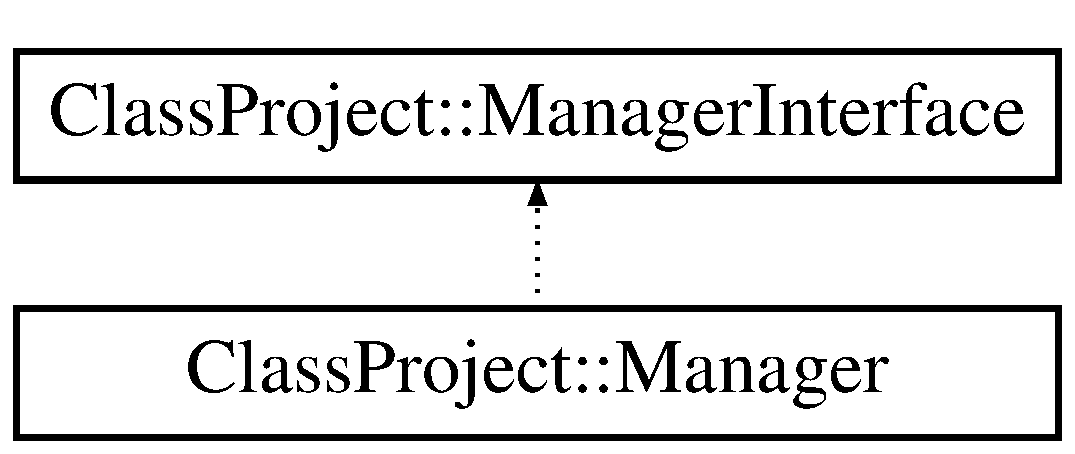
\includegraphics[height=2.000000cm]{classClassProject_1_1ManagerInterface}
\end{center}
\end{figure}
\subsection*{Public Member Functions}
\begin{DoxyCompactItemize}
\item 
virtual B\+D\+D\+\_\+\+ID {\bfseries create\+Var} (const std\+::string \&label)=0\label{classClassProject_1_1ManagerInterface_ab101acd3fbe6a5e29973d88f9862b8b4}

\item 
virtual const B\+D\+D\+\_\+\+ID \& {\bfseries True} ()=0\label{classClassProject_1_1ManagerInterface_a104d0e8bcbd81eb501b66db6e24d1f63}

\item 
virtual const B\+D\+D\+\_\+\+ID \& {\bfseries False} ()=0\label{classClassProject_1_1ManagerInterface_a98d18e1bc840fd664af015facfdcf690}

\item 
virtual bool {\bfseries is\+Constant} (const B\+D\+D\+\_\+\+ID f)=0\label{classClassProject_1_1ManagerInterface_a0edd879f6ecae7bc5f84a2d55373d977}

\item 
virtual bool {\bfseries is\+Variable} (const B\+D\+D\+\_\+\+ID x)=0\label{classClassProject_1_1ManagerInterface_a6eaaec7cbf8826198e490313ccb8f22a}

\item 
virtual B\+D\+D\+\_\+\+ID {\bfseries top\+Var} (const B\+D\+D\+\_\+\+ID f)=0\label{classClassProject_1_1ManagerInterface_ae2c645f859bcc7be3376d478f01eb045}

\item 
virtual B\+D\+D\+\_\+\+ID {\bfseries ite} (const B\+D\+D\+\_\+\+ID i, const B\+D\+D\+\_\+\+ID t, const B\+D\+D\+\_\+\+ID e)=0\label{classClassProject_1_1ManagerInterface_a6ea8f9482d86afb4128c52328d9ec11c}

\item 
virtual B\+D\+D\+\_\+\+ID {\bfseries co\+Factor\+True} (const B\+D\+D\+\_\+\+ID f, B\+D\+D\+\_\+\+ID x)=0\label{classClassProject_1_1ManagerInterface_aab8496a0e551abdad99160e152199f4b}

\item 
virtual B\+D\+D\+\_\+\+ID {\bfseries co\+Factor\+False} (const B\+D\+D\+\_\+\+ID f, B\+D\+D\+\_\+\+ID x)=0\label{classClassProject_1_1ManagerInterface_ad749ef1542c5b23bbbce628d6f666fe4}

\item 
virtual B\+D\+D\+\_\+\+ID {\bfseries co\+Factor\+True} (const B\+D\+D\+\_\+\+ID f)=0\label{classClassProject_1_1ManagerInterface_a4a1880d2245af9130646232551940949}

\item 
virtual B\+D\+D\+\_\+\+ID {\bfseries co\+Factor\+False} (const B\+D\+D\+\_\+\+ID f)=0\label{classClassProject_1_1ManagerInterface_a308c99661ad02f407d6f2b0af6230e80}

\item 
virtual B\+D\+D\+\_\+\+ID {\bfseries and2} (const B\+D\+D\+\_\+\+ID a, const B\+D\+D\+\_\+\+ID b)=0\label{classClassProject_1_1ManagerInterface_af914326d34a1ed42710f7b11e5baf010}

\item 
virtual B\+D\+D\+\_\+\+ID {\bfseries or2} (const B\+D\+D\+\_\+\+ID a, const B\+D\+D\+\_\+\+ID b)=0\label{classClassProject_1_1ManagerInterface_a8dbfde761b1e94d1f222b4d27f3c6fbc}

\item 
virtual B\+D\+D\+\_\+\+ID {\bfseries xor2} (const B\+D\+D\+\_\+\+ID a, const B\+D\+D\+\_\+\+ID b)=0\label{classClassProject_1_1ManagerInterface_a2b2c4948ef41ddb1036289cd07dac156}

\item 
virtual B\+D\+D\+\_\+\+ID {\bfseries neg} (const B\+D\+D\+\_\+\+ID a)=0\label{classClassProject_1_1ManagerInterface_a57d34af3121dcf5366d22ecf792f05a0}

\item 
virtual B\+D\+D\+\_\+\+ID {\bfseries nand2} (const B\+D\+D\+\_\+\+ID a, const B\+D\+D\+\_\+\+ID b)=0\label{classClassProject_1_1ManagerInterface_aaf6e357d680613e449d3ea958c9abba1}

\item 
virtual B\+D\+D\+\_\+\+ID {\bfseries nor2} (const B\+D\+D\+\_\+\+ID a, const B\+D\+D\+\_\+\+ID b)=0\label{classClassProject_1_1ManagerInterface_a312d9865eae2d6355e17855cba78bc78}

\item 
virtual std\+::string {\bfseries get\+Top\+Var\+Name} (const B\+D\+D\+\_\+\+ID \&root)=0\label{classClassProject_1_1ManagerInterface_afde45b2065361dfa6e61c1c7bc3fc1b4}

\item 
virtual void {\bfseries find\+Nodes} (const B\+D\+D\+\_\+\+ID \&root, std\+::set$<$ B\+D\+D\+\_\+\+ID $>$ \&nodes\+\_\+of\+\_\+root)=0\label{classClassProject_1_1ManagerInterface_ab460e331ffdb85d4128574b3aae72c1e}

\item 
virtual void {\bfseries find\+Vars} (const B\+D\+D\+\_\+\+ID \&root, std\+::set$<$ B\+D\+D\+\_\+\+ID $>$ \&vars\+\_\+of\+\_\+root)=0\label{classClassProject_1_1ManagerInterface_ab94feabca2125d334e542e502ae0186d}

\item 
virtual size\+\_\+t {\bfseries unique\+Table\+Size} ()=0\label{classClassProject_1_1ManagerInterface_a85cac80444b26e5b80eb96b9f1231c0e}

\end{DoxyCompactItemize}


The documentation for this class was generated from the following file\+:\begin{DoxyCompactItemize}
\item 
/import/home/vdscp04/\+Luiz/vdscp\+\_\+04/src/Manager\+Interface.\+h\end{DoxyCompactItemize}

\section{node Struct Reference}
\label{structnode}\index{node@{node}}
\subsection*{Public Attributes}
\begin{DoxyCompactItemize}
\item 
std\+::string {\bfseries var\+\_\+name}\label{structnode_a6a26f5e7101293a34704c34ab2b8846f}

\item 
int {\bfseries var\+\_\+id}\label{structnode_a9349fd79d66c48b710644e0833b8d316}

\item 
int {\bfseries low}\label{structnode_a10be3a6d1a2699623bebe2e3b49eff08}

\item 
int {\bfseries high}\label{structnode_a87e109220475573c3aedddb10b68dc45}

\end{DoxyCompactItemize}


The documentation for this struct was generated from the following file\+:\begin{DoxyCompactItemize}
\item 
/import/home/vdscp04/\+Luiz/vdscp\+\_\+04/src/verify/main\+\_\+verify.\+cpp\end{DoxyCompactItemize}

\section{Open\+File\+Exception Class Reference}
\label{classOpenFileException}\index{Open\+File\+Exception@{Open\+File\+Exception}}


This exception should be thrown when a file cannot be accessed.  




{\ttfamily \#include $<$bench\+\_\+circuit\+\_\+manager.\+hpp$>$}

Inheritance diagram for Open\+File\+Exception\+:\begin{figure}[H]
\begin{center}
\leavevmode
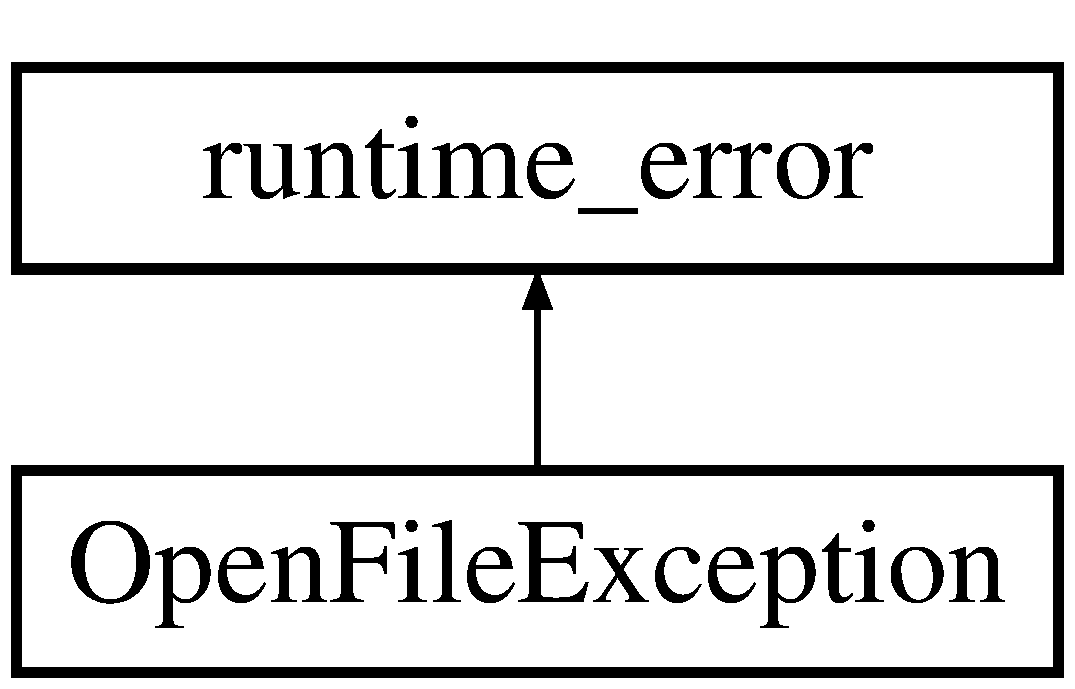
\includegraphics[height=2.000000cm]{classOpenFileException}
\end{center}
\end{figure}
\subsection*{Public Member Functions}
\begin{DoxyCompactItemize}
\item 
{\bfseries Open\+File\+Exception} (const std\+::string \&message)\label{classOpenFileException_a6632ca961e00571c690b071d033651e7}

\end{DoxyCompactItemize}


\subsection{Detailed Description}
This exception should be thrown when a file cannot be accessed. 

The documentation for this class was generated from the following file\+:\begin{DoxyCompactItemize}
\item 
/home/felipe/\+Desktop/vdsproject/vdscp\+\_\+04/src/bench/bench\+\_\+circuit\+\_\+manager.\+hpp\end{DoxyCompactItemize}

\section{ska\+:\+:power\+\_\+of\+\_\+two\+\_\+hash\+\_\+policy Struct Reference}
\label{structska_1_1power__of__two__hash__policy}\index{ska\+::power\+\_\+of\+\_\+two\+\_\+hash\+\_\+policy@{ska\+::power\+\_\+of\+\_\+two\+\_\+hash\+\_\+policy}}
\subsection*{Public Member Functions}
\begin{DoxyCompactItemize}
\item 
size\+\_\+t {\bfseries index\+\_\+for\+\_\+hash} (size\+\_\+t hash, size\+\_\+t num\+\_\+slots\+\_\+minus\+\_\+one) const \label{structska_1_1power__of__two__hash__policy_a00ff8699ccb31f173a4e61e1c7b70754}

\item 
int8\+\_\+t {\bfseries next\+\_\+size\+\_\+over} (size\+\_\+t \&size) const \label{structska_1_1power__of__two__hash__policy_a549ddfd949be3f587c49f7554778f3f9}

\item 
void {\bfseries commit} (int8\+\_\+t)\label{structska_1_1power__of__two__hash__policy_a53b77defec0ddede94abdf6c97f463d6}

\item 
void {\bfseries reset} ()\label{structska_1_1power__of__two__hash__policy_aae69bae44c4a35e0f45f18ed09b12c22}

\end{DoxyCompactItemize}


The documentation for this struct was generated from the following file\+:\begin{DoxyCompactItemize}
\item 
/home/felipe/\+Desktop/vdsproject/vdscp\+\_\+04/src/flat\+\_\+hash\+\_\+map.\+hpp\end{DoxyCompactItemize}

\section{ska\+:\+:power\+\_\+of\+\_\+two\+\_\+std\+\_\+hash$<$ T $>$ Struct Template Reference}
\label{structska_1_1power__of__two__std__hash}\index{ska\+::power\+\_\+of\+\_\+two\+\_\+std\+\_\+hash$<$ T $>$@{ska\+::power\+\_\+of\+\_\+two\+\_\+std\+\_\+hash$<$ T $>$}}
Inheritance diagram for ska\+:\+:power\+\_\+of\+\_\+two\+\_\+std\+\_\+hash$<$ T $>$\+:\begin{figure}[H]
\begin{center}
\leavevmode
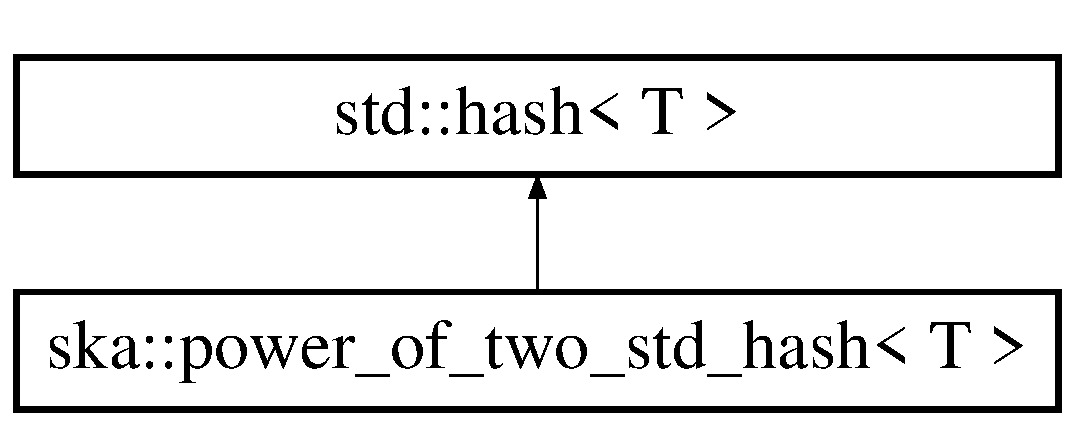
\includegraphics[height=2.000000cm]{structska_1_1power__of__two__std__hash}
\end{center}
\end{figure}
\subsection*{Public Types}
\begin{DoxyCompactItemize}
\item 
typedef {\bf ska\+::power\+\_\+of\+\_\+two\+\_\+hash\+\_\+policy} {\bfseries hash\+\_\+policy}\label{structska_1_1power__of__two__std__hash_a47c92f03fb274333eb6bf590cfc472b4}

\end{DoxyCompactItemize}


The documentation for this struct was generated from the following file\+:\begin{DoxyCompactItemize}
\item 
/home/felipe/\+Desktop/vdsproject/vdscp\+\_\+04/src/flat\+\_\+hash\+\_\+map.\+hpp\end{DoxyCompactItemize}

\section{ska\+:\+:prime\+\_\+number\+\_\+hash\+\_\+policy Struct Reference}
\label{structska_1_1prime__number__hash__policy}\index{ska\+::prime\+\_\+number\+\_\+hash\+\_\+policy@{ska\+::prime\+\_\+number\+\_\+hash\+\_\+policy}}
\subsection*{Public Member Functions}
\begin{DoxyCompactItemize}
\item 
size\+\_\+t {\bfseries index\+\_\+for\+\_\+hash} (size\+\_\+t hash, size\+\_\+t) const \label{structska_1_1prime__number__hash__policy_a474304979d54425a2530a5a11321881b}

\item 
uint8\+\_\+t {\bfseries next\+\_\+size\+\_\+over} (size\+\_\+t \&size) const \label{structska_1_1prime__number__hash__policy_a2677e5405639125b7c27cd412555b7ea}

\item 
void {\bfseries commit} (uint8\+\_\+t new\+\_\+prime\+\_\+index)\label{structska_1_1prime__number__hash__policy_a8b3a847f42f0ee4c5acbdf5c7acd1598}

\item 
void {\bfseries reset} ()\label{structska_1_1prime__number__hash__policy_ae70c41a3db310936504c0a3eb07c4395}

\end{DoxyCompactItemize}
\subsection*{Static Public Member Functions}
\begin{DoxyCompactItemize}
\item 
static size\+\_\+t {\bfseries mod0} (size\+\_\+t)\label{structska_1_1prime__number__hash__policy_a1fb36bb689ba60d13aa22bebc11981b3}

\item 
static size\+\_\+t {\bfseries mod2} (size\+\_\+t hash)\label{structska_1_1prime__number__hash__policy_a536a0b1fb60552e5ac663ab297545fef}

\item 
static size\+\_\+t {\bfseries mod3} (size\+\_\+t hash)\label{structska_1_1prime__number__hash__policy_a15277115155734a5be6682722945cb71}

\item 
static size\+\_\+t {\bfseries mod5} (size\+\_\+t hash)\label{structska_1_1prime__number__hash__policy_a4ac36e6d414043b4aaf25ed1ae59ad0e}

\item 
static size\+\_\+t {\bfseries mod7} (size\+\_\+t hash)\label{structska_1_1prime__number__hash__policy_a988650288dd42b5cbb037767b3ca0b5c}

\item 
static size\+\_\+t {\bfseries mod11} (size\+\_\+t hash)\label{structska_1_1prime__number__hash__policy_a23aed78772f573194dd6b228d2beb738}

\item 
static size\+\_\+t {\bfseries mod13} (size\+\_\+t hash)\label{structska_1_1prime__number__hash__policy_a2de51f11b798fb102f0a5efc469d012d}

\item 
static size\+\_\+t {\bfseries mod17} (size\+\_\+t hash)\label{structska_1_1prime__number__hash__policy_a8183640d818c1a6458950e1ca01b396d}

\item 
static size\+\_\+t {\bfseries mod23} (size\+\_\+t hash)\label{structska_1_1prime__number__hash__policy_a98e3e7fd2cdc181105e02d4792ec8e55}

\item 
static size\+\_\+t {\bfseries mod29} (size\+\_\+t hash)\label{structska_1_1prime__number__hash__policy_a56281c42d12b6552bf0ddbb5f578ec97}

\item 
static size\+\_\+t {\bfseries mod37} (size\+\_\+t hash)\label{structska_1_1prime__number__hash__policy_a311811627df3acb8d57deb8ea306f027}

\item 
static size\+\_\+t {\bfseries mod47} (size\+\_\+t hash)\label{structska_1_1prime__number__hash__policy_aea326c7d1dce5ca6271796776fb2c0ac}

\item 
static size\+\_\+t {\bfseries mod59} (size\+\_\+t hash)\label{structska_1_1prime__number__hash__policy_a4c0d0b3e4cf664e2492eb4cd66e060fb}

\item 
static size\+\_\+t {\bfseries mod73} (size\+\_\+t hash)\label{structska_1_1prime__number__hash__policy_acd79944e2ed6ec749b3059755ad105a8}

\item 
static size\+\_\+t {\bfseries mod97} (size\+\_\+t hash)\label{structska_1_1prime__number__hash__policy_ac39ce7b1a7e3fc5faa9db2b3940c27b5}

\item 
static size\+\_\+t {\bfseries mod127} (size\+\_\+t hash)\label{structska_1_1prime__number__hash__policy_af02a9e99adbcecbd1dc21d776a23271a}

\item 
static size\+\_\+t {\bfseries mod151} (size\+\_\+t hash)\label{structska_1_1prime__number__hash__policy_a9bd8959a8c34db811e9dab2bdacade3b}

\item 
static size\+\_\+t {\bfseries mod197} (size\+\_\+t hash)\label{structska_1_1prime__number__hash__policy_a1133c263f46f835ea5733995bafcf727}

\item 
static size\+\_\+t {\bfseries mod251} (size\+\_\+t hash)\label{structska_1_1prime__number__hash__policy_a01b39c17298f1d3f5e263067a522a14d}

\item 
static size\+\_\+t {\bfseries mod313} (size\+\_\+t hash)\label{structska_1_1prime__number__hash__policy_ab5ad132597c13594b9e1d5ecc8199cd4}

\item 
static size\+\_\+t {\bfseries mod397} (size\+\_\+t hash)\label{structska_1_1prime__number__hash__policy_a5c6cf8584148db70ffae94bfccf9700e}

\item 
static size\+\_\+t {\bfseries mod499} (size\+\_\+t hash)\label{structska_1_1prime__number__hash__policy_af8fde6c342c10b0648d0869540fe0993}

\item 
static size\+\_\+t {\bfseries mod631} (size\+\_\+t hash)\label{structska_1_1prime__number__hash__policy_a325a81b54e2b9355d3a94397f9d492f8}

\item 
static size\+\_\+t {\bfseries mod797} (size\+\_\+t hash)\label{structska_1_1prime__number__hash__policy_a7d984074338e1cf49a9eb7689cb27c96}

\item 
static size\+\_\+t {\bfseries mod1009} (size\+\_\+t hash)\label{structska_1_1prime__number__hash__policy_ab3d528eebef644012481e3a43e5e1b33}

\item 
static size\+\_\+t {\bfseries mod1259} (size\+\_\+t hash)\label{structska_1_1prime__number__hash__policy_a1535eff52bdaaeb76605c079612dd4a9}

\item 
static size\+\_\+t {\bfseries mod1597} (size\+\_\+t hash)\label{structska_1_1prime__number__hash__policy_a1e9a446fb8ee06508bf0369626bcbb1c}

\item 
static size\+\_\+t {\bfseries mod2011} (size\+\_\+t hash)\label{structska_1_1prime__number__hash__policy_a1caa651204657248b48e411268dcfb47}

\item 
static size\+\_\+t {\bfseries mod2539} (size\+\_\+t hash)\label{structska_1_1prime__number__hash__policy_a82807ddcf07933ef585fda159dfc3020}

\item 
static size\+\_\+t {\bfseries mod3203} (size\+\_\+t hash)\label{structska_1_1prime__number__hash__policy_a322d2d4cc0079540bbe46ce1d57a1d71}

\item 
static size\+\_\+t {\bfseries mod4027} (size\+\_\+t hash)\label{structska_1_1prime__number__hash__policy_acdba7984a9862983a4acb86448e94252}

\item 
static size\+\_\+t {\bfseries mod5087} (size\+\_\+t hash)\label{structska_1_1prime__number__hash__policy_a8de1e0c23833b2404d5ff1441d3db656}

\item 
static size\+\_\+t {\bfseries mod6421} (size\+\_\+t hash)\label{structska_1_1prime__number__hash__policy_a23813640b8ad7a5f32eb0bafdbd11577}

\item 
static size\+\_\+t {\bfseries mod8089} (size\+\_\+t hash)\label{structska_1_1prime__number__hash__policy_ae22353d02e9b3fdf7af2c7b7c36ce2d9}

\item 
static size\+\_\+t {\bfseries mod10193} (size\+\_\+t hash)\label{structska_1_1prime__number__hash__policy_ae1775bee48c2d6446d10871066f58c6a}

\item 
static size\+\_\+t {\bfseries mod12853} (size\+\_\+t hash)\label{structska_1_1prime__number__hash__policy_a0344e9af15e7488f83efc845fd2e6bcd}

\item 
static size\+\_\+t {\bfseries mod16193} (size\+\_\+t hash)\label{structska_1_1prime__number__hash__policy_a968793384ed9ef0171bcb057ed42337a}

\item 
static size\+\_\+t {\bfseries mod20399} (size\+\_\+t hash)\label{structska_1_1prime__number__hash__policy_aa1b5839a21759fa112eedd65264ef617}

\item 
static size\+\_\+t {\bfseries mod25717} (size\+\_\+t hash)\label{structska_1_1prime__number__hash__policy_afeab6d5dcacdaf736d4972915398096b}

\item 
static size\+\_\+t {\bfseries mod32401} (size\+\_\+t hash)\label{structska_1_1prime__number__hash__policy_a64b9b40985fd79e54a3bd1e6378f5e77}

\item 
static size\+\_\+t {\bfseries mod40823} (size\+\_\+t hash)\label{structska_1_1prime__number__hash__policy_a0f8d6844e667972f7726672c82de3bef}

\item 
static size\+\_\+t {\bfseries mod51437} (size\+\_\+t hash)\label{structska_1_1prime__number__hash__policy_ab7d5cea78bffcac78f9197ef8797c92e}

\item 
static size\+\_\+t {\bfseries mod64811} (size\+\_\+t hash)\label{structska_1_1prime__number__hash__policy_abf329eeba30aae5deb594cd82668f200}

\item 
static size\+\_\+t {\bfseries mod81649} (size\+\_\+t hash)\label{structska_1_1prime__number__hash__policy_a0fa2b4ba20d67ae91e8bccb9bb24d29d}

\item 
static size\+\_\+t {\bfseries mod102877} (size\+\_\+t hash)\label{structska_1_1prime__number__hash__policy_aeee1369c3bcbf482389bc6d3602f65b8}

\item 
static size\+\_\+t {\bfseries mod129607} (size\+\_\+t hash)\label{structska_1_1prime__number__hash__policy_a1307177624372139556de2408e38e203}

\item 
static size\+\_\+t {\bfseries mod163307} (size\+\_\+t hash)\label{structska_1_1prime__number__hash__policy_a3170fcc205243a430c671e60310cdd98}

\item 
static size\+\_\+t {\bfseries mod205759} (size\+\_\+t hash)\label{structska_1_1prime__number__hash__policy_a0d54457b4ec5dfc31af1365f86a7dc36}

\item 
static size\+\_\+t {\bfseries mod259229} (size\+\_\+t hash)\label{structska_1_1prime__number__hash__policy_a0e546081995005fe117e9395b9ddcb09}

\item 
static size\+\_\+t {\bfseries mod326617} (size\+\_\+t hash)\label{structska_1_1prime__number__hash__policy_a0359c18d304e0e1c66fc79fbb6581e03}

\item 
static size\+\_\+t {\bfseries mod411527} (size\+\_\+t hash)\label{structska_1_1prime__number__hash__policy_ae359e734efb85a7215f7934c032d9553}

\item 
static size\+\_\+t {\bfseries mod518509} (size\+\_\+t hash)\label{structska_1_1prime__number__hash__policy_a0ab2660c0df51f19fc2968b4f73bc660}

\item 
static size\+\_\+t {\bfseries mod653267} (size\+\_\+t hash)\label{structska_1_1prime__number__hash__policy_a1621841fce8d8e6b83aac9c212cd67cd}

\item 
static size\+\_\+t {\bfseries mod823117} (size\+\_\+t hash)\label{structska_1_1prime__number__hash__policy_a006068c645ec6704b7973cb4ebb38f19}

\item 
static size\+\_\+t {\bfseries mod1037059} (size\+\_\+t hash)\label{structska_1_1prime__number__hash__policy_ad7317d582c8338ae714c68ba9fc87fe6}

\item 
static size\+\_\+t {\bfseries mod1306601} (size\+\_\+t hash)\label{structska_1_1prime__number__hash__policy_a6cd73834afc77f8b8653aeeea29882a7}

\item 
static size\+\_\+t {\bfseries mod1646237} (size\+\_\+t hash)\label{structska_1_1prime__number__hash__policy_af23e2f41687d2d49f95aa479be71f39f}

\item 
static size\+\_\+t {\bfseries mod2074129} (size\+\_\+t hash)\label{structska_1_1prime__number__hash__policy_a84871bf07f2a3087aa930d7812f3d0db}

\item 
static size\+\_\+t {\bfseries mod2613229} (size\+\_\+t hash)\label{structska_1_1prime__number__hash__policy_af4ff19b682a8d71fbfe269d0f28a5369}

\item 
static size\+\_\+t {\bfseries mod3292489} (size\+\_\+t hash)\label{structska_1_1prime__number__hash__policy_a522ceab5bbfaf9215bfb4dc08912ff42}

\item 
static size\+\_\+t {\bfseries mod4148279} (size\+\_\+t hash)\label{structska_1_1prime__number__hash__policy_a90dea8ac4fb413740bc2d1e8238a4643}

\item 
static size\+\_\+t {\bfseries mod5226491} (size\+\_\+t hash)\label{structska_1_1prime__number__hash__policy_af5006b3510982acc8ce58f058a6e949b}

\item 
static size\+\_\+t {\bfseries mod6584983} (size\+\_\+t hash)\label{structska_1_1prime__number__hash__policy_a346919955b2815d3e5c7a93e0720645a}

\item 
static size\+\_\+t {\bfseries mod8296553} (size\+\_\+t hash)\label{structska_1_1prime__number__hash__policy_a63d21d25dd55f6381c505e6838959122}

\item 
static size\+\_\+t {\bfseries mod10453007} (size\+\_\+t hash)\label{structska_1_1prime__number__hash__policy_aaeabebf2fbca6fbae1def66924433864}

\item 
static size\+\_\+t {\bfseries mod13169977} (size\+\_\+t hash)\label{structska_1_1prime__number__hash__policy_aeed2b0a6e871d899aa66c8e20be223a0}

\item 
static size\+\_\+t {\bfseries mod16593127} (size\+\_\+t hash)\label{structska_1_1prime__number__hash__policy_ac482cbe8f036f926ae8226be01997c18}

\item 
static size\+\_\+t {\bfseries mod20906033} (size\+\_\+t hash)\label{structska_1_1prime__number__hash__policy_a1559a4f6eb749baa639afa3234b4507e}

\item 
static size\+\_\+t {\bfseries mod26339969} (size\+\_\+t hash)\label{structska_1_1prime__number__hash__policy_a16466b7fba8b4aa8e8005bed702551e5}

\item 
static size\+\_\+t {\bfseries mod33186281} (size\+\_\+t hash)\label{structska_1_1prime__number__hash__policy_adfa33c7eb09b5e16d47bd4aacadff263}

\item 
static size\+\_\+t {\bfseries mod41812097} (size\+\_\+t hash)\label{structska_1_1prime__number__hash__policy_a19bd140b945234db7ccea3d94c7a2468}

\item 
static size\+\_\+t {\bfseries mod52679969} (size\+\_\+t hash)\label{structska_1_1prime__number__hash__policy_a7ae3974a52c376eb8c4736b8aa388d8b}

\item 
static size\+\_\+t {\bfseries mod66372617} (size\+\_\+t hash)\label{structska_1_1prime__number__hash__policy_afca57792ed6a4f497b4939adb24bc5e0}

\item 
static size\+\_\+t {\bfseries mod83624237} (size\+\_\+t hash)\label{structska_1_1prime__number__hash__policy_add30783edec4f53a3b1f388ab9603400}

\item 
static size\+\_\+t {\bfseries mod105359939} (size\+\_\+t hash)\label{structska_1_1prime__number__hash__policy_a18fc27f5802a3bd1b7cdbae04c65c03d}

\item 
static size\+\_\+t {\bfseries mod132745199} (size\+\_\+t hash)\label{structska_1_1prime__number__hash__policy_a0e0257d76a701522349d334e70283c6e}

\item 
static size\+\_\+t {\bfseries mod167248483} (size\+\_\+t hash)\label{structska_1_1prime__number__hash__policy_a890b8930ca9d40f8311205228b003646}

\item 
static size\+\_\+t {\bfseries mod210719881} (size\+\_\+t hash)\label{structska_1_1prime__number__hash__policy_a9b1ffc15af001616baa25f83c98ba4ef}

\item 
static size\+\_\+t {\bfseries mod265490441} (size\+\_\+t hash)\label{structska_1_1prime__number__hash__policy_ab26a11b5d9067e7a70a52cedca329fb2}

\item 
static size\+\_\+t {\bfseries mod334496971} (size\+\_\+t hash)\label{structska_1_1prime__number__hash__policy_a4061c26f2697de407974971095352dba}

\item 
static size\+\_\+t {\bfseries mod421439783} (size\+\_\+t hash)\label{structska_1_1prime__number__hash__policy_a4313f6a84c6e79a9559eaf3756457aee}

\item 
static size\+\_\+t {\bfseries mod530980861} (size\+\_\+t hash)\label{structska_1_1prime__number__hash__policy_abe5cab5659a76347a15aa1246c1f8eb2}

\item 
static size\+\_\+t {\bfseries mod668993977} (size\+\_\+t hash)\label{structska_1_1prime__number__hash__policy_aa7fbf9b6b09f824059cb59475799ba75}

\item 
static size\+\_\+t {\bfseries mod842879579} (size\+\_\+t hash)\label{structska_1_1prime__number__hash__policy_ab56114f474f578a4e54548e8ea99c696}

\item 
static size\+\_\+t {\bfseries mod1061961721} (size\+\_\+t hash)\label{structska_1_1prime__number__hash__policy_a95e55c433d285c2a210785f486eca5d7}

\item 
static size\+\_\+t {\bfseries mod1337987929} (size\+\_\+t hash)\label{structska_1_1prime__number__hash__policy_aeddd4cff87d37cf140a775464ceaa6b1}

\item 
static size\+\_\+t {\bfseries mod1685759167} (size\+\_\+t hash)\label{structska_1_1prime__number__hash__policy_a822bec93f0fa19ac6bc2fcd5baecf9bf}

\item 
static size\+\_\+t {\bfseries mod2123923447} (size\+\_\+t hash)\label{structska_1_1prime__number__hash__policy_aa8a78b03772363e48c1de9ace0d7f528}

\item 
static size\+\_\+t {\bfseries mod2675975881} (size\+\_\+t hash)\label{structska_1_1prime__number__hash__policy_aad231869eb2522a7d8a2b53f5f868ac2}

\item 
static size\+\_\+t {\bfseries mod3371518343} (size\+\_\+t hash)\label{structska_1_1prime__number__hash__policy_a2062fdc13622eb38e02c8a9e0676c24e}

\item 
static size\+\_\+t {\bfseries mod4247846927} (size\+\_\+t hash)\label{structska_1_1prime__number__hash__policy_a443cef06d6d6f9b824ed160f63c8fafb}

\item 
static size\+\_\+t {\bfseries mod5351951779} (size\+\_\+t hash)\label{structska_1_1prime__number__hash__policy_aa663c6629e5f8335112052ecc31223d8}

\item 
static size\+\_\+t {\bfseries mod6743036717} (size\+\_\+t hash)\label{structska_1_1prime__number__hash__policy_af9afe88084bf9f614e5e85190bc91393}

\item 
static size\+\_\+t {\bfseries mod8495693897} (size\+\_\+t hash)\label{structska_1_1prime__number__hash__policy_a4247ef31ca2e92948446a7a9c84ad1e4}

\item 
static size\+\_\+t {\bfseries mod10703903591} (size\+\_\+t hash)\label{structska_1_1prime__number__hash__policy_a724b676895bfca6dfe1af26c1ee3b91a}

\item 
static size\+\_\+t {\bfseries mod13486073473} (size\+\_\+t hash)\label{structska_1_1prime__number__hash__policy_a0ebfe5f0edcff9edbace3f309c2f7c29}

\item 
static size\+\_\+t {\bfseries mod16991387857} (size\+\_\+t hash)\label{structska_1_1prime__number__hash__policy_aa13812835b4868cccf6338de273c512a}

\item 
static size\+\_\+t {\bfseries mod21407807219} (size\+\_\+t hash)\label{structska_1_1prime__number__hash__policy_a9049bd704f91aff562d472fd03820004}

\item 
static size\+\_\+t {\bfseries mod26972146961} (size\+\_\+t hash)\label{structska_1_1prime__number__hash__policy_a5e6dbf8dde39e5ee1b9a91cafe99a5a4}

\item 
static size\+\_\+t {\bfseries mod33982775741} (size\+\_\+t hash)\label{structska_1_1prime__number__hash__policy_a4ad7bf3f54661f5b3bbbdea7cb216394}

\item 
static size\+\_\+t {\bfseries mod42815614441} (size\+\_\+t hash)\label{structska_1_1prime__number__hash__policy_a03529f67b9d1348c343086f547cd2782}

\item 
static size\+\_\+t {\bfseries mod53944293929} (size\+\_\+t hash)\label{structska_1_1prime__number__hash__policy_a0a22d5ef1773d32de1326bbb1947205b}

\item 
static size\+\_\+t {\bfseries mod67965551447} (size\+\_\+t hash)\label{structska_1_1prime__number__hash__policy_a1c5d85541af5627be165543f90a07040}

\item 
static size\+\_\+t {\bfseries mod85631228929} (size\+\_\+t hash)\label{structska_1_1prime__number__hash__policy_a1e8e0cd8957461e4edfca04150b17e0a}

\item 
static size\+\_\+t {\bfseries mod107888587883} (size\+\_\+t hash)\label{structska_1_1prime__number__hash__policy_ae3917bf56f4033d912cbf66c245faee5}

\item 
static size\+\_\+t {\bfseries mod135931102921} (size\+\_\+t hash)\label{structska_1_1prime__number__hash__policy_adea39cb6a9d83bb996a16afaa5c1d96c}

\item 
static size\+\_\+t {\bfseries mod171262457903} (size\+\_\+t hash)\label{structska_1_1prime__number__hash__policy_a4d61d6c942c4243896d9b49880533bb7}

\item 
static size\+\_\+t {\bfseries mod215777175787} (size\+\_\+t hash)\label{structska_1_1prime__number__hash__policy_a508a41e218eb9544ff841bb185d5a8d0}

\item 
static size\+\_\+t {\bfseries mod271862205833} (size\+\_\+t hash)\label{structska_1_1prime__number__hash__policy_a95f1575f404f2f0b5dd37a9a12dce8c2}

\item 
static size\+\_\+t {\bfseries mod342524915839} (size\+\_\+t hash)\label{structska_1_1prime__number__hash__policy_acac67709378e5402de5037bdc7754b62}

\item 
static size\+\_\+t {\bfseries mod431554351609} (size\+\_\+t hash)\label{structska_1_1prime__number__hash__policy_a3cf2c4f2c2becf50b470b693f4a1e237}

\item 
static size\+\_\+t {\bfseries mod543724411781} (size\+\_\+t hash)\label{structska_1_1prime__number__hash__policy_ae641d1d595c6cd788e8f69b0413ba3a7}

\item 
static size\+\_\+t {\bfseries mod685049831731} (size\+\_\+t hash)\label{structska_1_1prime__number__hash__policy_ad184c8bae353ab65f9bc01e977be0ae2}

\item 
static size\+\_\+t {\bfseries mod863108703229} (size\+\_\+t hash)\label{structska_1_1prime__number__hash__policy_ab02bddc25d3f5afd91d30ee205370c06}

\item 
static size\+\_\+t {\bfseries mod1087448823553} (size\+\_\+t hash)\label{structska_1_1prime__number__hash__policy_acb45f2c723fcf140ffad28e8897b754f}

\item 
static size\+\_\+t {\bfseries mod1370099663459} (size\+\_\+t hash)\label{structska_1_1prime__number__hash__policy_afb903af889e634f2270454fe342021b2}

\item 
static size\+\_\+t {\bfseries mod1726217406467} (size\+\_\+t hash)\label{structska_1_1prime__number__hash__policy_a49b21b5dd337d587f9ae785603d3e21c}

\item 
static size\+\_\+t {\bfseries mod2174897647073} (size\+\_\+t hash)\label{structska_1_1prime__number__hash__policy_a0aaefe43940c78b17fab14d24393c236}

\item 
static size\+\_\+t {\bfseries mod2740199326961} (size\+\_\+t hash)\label{structska_1_1prime__number__hash__policy_a796f27ca1ddf0fd16da5feb700f3e9bc}

\item 
static size\+\_\+t {\bfseries mod3452434812973} (size\+\_\+t hash)\label{structska_1_1prime__number__hash__policy_a87d23f8866d3714662ff3cf6dc528413}

\item 
static size\+\_\+t {\bfseries mod4349795294267} (size\+\_\+t hash)\label{structska_1_1prime__number__hash__policy_a21a46e5ede8398becb4f78731c5d194f}

\item 
static size\+\_\+t {\bfseries mod5480398654009} (size\+\_\+t hash)\label{structska_1_1prime__number__hash__policy_a0dba43d09a1f1f1beda5a2e0d4800445}

\item 
static size\+\_\+t {\bfseries mod6904869625999} (size\+\_\+t hash)\label{structska_1_1prime__number__hash__policy_aaadce39c853108f4a1650e1c1fb0e504}

\item 
static size\+\_\+t {\bfseries mod8699590588571} (size\+\_\+t hash)\label{structska_1_1prime__number__hash__policy_ad3c33e3a76e079ff4b879ecaede43dc7}

\item 
static size\+\_\+t {\bfseries mod10960797308051} (size\+\_\+t hash)\label{structska_1_1prime__number__hash__policy_afb652145e8b0e92d5f75bc886ef2a560}

\item 
static size\+\_\+t {\bfseries mod13809739252051} (size\+\_\+t hash)\label{structska_1_1prime__number__hash__policy_ae56f594f8b0adf15401fb7427e083054}

\item 
static size\+\_\+t {\bfseries mod17399181177241} (size\+\_\+t hash)\label{structska_1_1prime__number__hash__policy_acff3919d52a920152b56501a1d520687}

\item 
static size\+\_\+t {\bfseries mod21921594616111} (size\+\_\+t hash)\label{structska_1_1prime__number__hash__policy_ade423084add1fbd6628598d895ad6e7d}

\item 
static size\+\_\+t {\bfseries mod27619478504183} (size\+\_\+t hash)\label{structska_1_1prime__number__hash__policy_aeed533fc80e47c39f33f48f07d5a39a6}

\item 
static size\+\_\+t {\bfseries mod34798362354533} (size\+\_\+t hash)\label{structska_1_1prime__number__hash__policy_a2cc5d14b084d02f9924bbaff8c6efe1e}

\item 
static size\+\_\+t {\bfseries mod43843189232363} (size\+\_\+t hash)\label{structska_1_1prime__number__hash__policy_afad91d1e62351df6c0e1953bb413247b}

\item 
static size\+\_\+t {\bfseries mod55238957008387} (size\+\_\+t hash)\label{structska_1_1prime__number__hash__policy_acdc27e29a073cf05373dc1298f736a84}

\item 
static size\+\_\+t {\bfseries mod69596724709081} (size\+\_\+t hash)\label{structska_1_1prime__number__hash__policy_a760e8cc50a87d5d489cbfaee2fd6bc1e}

\item 
static size\+\_\+t {\bfseries mod87686378464759} (size\+\_\+t hash)\label{structska_1_1prime__number__hash__policy_a09087ab6adb75b0c4bef5ed5b7f7d82f}

\item 
static size\+\_\+t {\bfseries mod110477914016779} (size\+\_\+t hash)\label{structska_1_1prime__number__hash__policy_ab4c42b8aa329ce3f6c83f98e637dfb0a}

\item 
static size\+\_\+t {\bfseries mod139193449418173} (size\+\_\+t hash)\label{structska_1_1prime__number__hash__policy_ab3e6639ae84e84357008db116ff227af}

\item 
static size\+\_\+t {\bfseries mod175372756929481} (size\+\_\+t hash)\label{structska_1_1prime__number__hash__policy_ae151c5885f656fe3b8ee6b5097f6b569}

\item 
static size\+\_\+t {\bfseries mod220955828033581} (size\+\_\+t hash)\label{structska_1_1prime__number__hash__policy_af03982d0f4f836432720c38b044a5aee}

\item 
static size\+\_\+t {\bfseries mod278386898836457} (size\+\_\+t hash)\label{structska_1_1prime__number__hash__policy_ae3b9920a47ae22e20470ba5f331cafc9}

\item 
static size\+\_\+t {\bfseries mod350745513859007} (size\+\_\+t hash)\label{structska_1_1prime__number__hash__policy_a76f9e81336d03916f1a60d4a68129447}

\item 
static size\+\_\+t {\bfseries mod441911656067171} (size\+\_\+t hash)\label{structska_1_1prime__number__hash__policy_a8c58fed5c96653fc0d44fdc4c8608f6b}

\item 
static size\+\_\+t {\bfseries mod556773797672909} (size\+\_\+t hash)\label{structska_1_1prime__number__hash__policy_ae7a7159cc3a3d5de3d896d6d72748537}

\item 
static size\+\_\+t {\bfseries mod701491027718027} (size\+\_\+t hash)\label{structska_1_1prime__number__hash__policy_afde91e3311a3d10d485842aeccfae7b6}

\item 
static size\+\_\+t {\bfseries mod883823312134381} (size\+\_\+t hash)\label{structska_1_1prime__number__hash__policy_a7b21fa1d003f8481ad39877b1e969db0}

\item 
static size\+\_\+t {\bfseries mod1113547595345903} (size\+\_\+t hash)\label{structska_1_1prime__number__hash__policy_a8fbc68a50635ec541b02de99768a8c73}

\item 
static size\+\_\+t {\bfseries mod1402982055436147} (size\+\_\+t hash)\label{structska_1_1prime__number__hash__policy_aede3f70e62e8713ecc7fb8b3b20a86bc}

\item 
static size\+\_\+t {\bfseries mod1767646624268779} (size\+\_\+t hash)\label{structska_1_1prime__number__hash__policy_ab8f9496a378c3ad33148a074d3d024b5}

\item 
static size\+\_\+t {\bfseries mod2227095190691797} (size\+\_\+t hash)\label{structska_1_1prime__number__hash__policy_a724fa57eb05e33747c7c603eff619b5d}

\item 
static size\+\_\+t {\bfseries mod2805964110872297} (size\+\_\+t hash)\label{structska_1_1prime__number__hash__policy_a0d055ce889eae8427b94e6b1d0606dc9}

\item 
static size\+\_\+t {\bfseries mod3535293248537579} (size\+\_\+t hash)\label{structska_1_1prime__number__hash__policy_a23cc1f29405a176a0fde281501757496}

\item 
static size\+\_\+t {\bfseries mod4454190381383713} (size\+\_\+t hash)\label{structska_1_1prime__number__hash__policy_a9f0f00d240cde043c1797a91c51f08a3}

\item 
static size\+\_\+t {\bfseries mod5611928221744609} (size\+\_\+t hash)\label{structska_1_1prime__number__hash__policy_a31efd844e9056b174727123a8496ebba}

\item 
static size\+\_\+t {\bfseries mod7070586497075177} (size\+\_\+t hash)\label{structska_1_1prime__number__hash__policy_a5c7b7f3fe0c28aa2ee33bfc849217a44}

\item 
static size\+\_\+t {\bfseries mod8908380762767489} (size\+\_\+t hash)\label{structska_1_1prime__number__hash__policy_aa5a9c3debbcb54db47eafcece3b53f2c}

\item 
static size\+\_\+t {\bfseries mod11223856443489329} (size\+\_\+t hash)\label{structska_1_1prime__number__hash__policy_a9d12f72e26fe2e315c113e1f4879939d}

\item 
static size\+\_\+t {\bfseries mod14141172994150357} (size\+\_\+t hash)\label{structska_1_1prime__number__hash__policy_adcd2db337628ae6eda8251b12090cec6}

\item 
static size\+\_\+t {\bfseries mod17816761525534927} (size\+\_\+t hash)\label{structska_1_1prime__number__hash__policy_a2e0b3e67f5097b6635df3cf96a96e7df}

\item 
static size\+\_\+t {\bfseries mod22447712886978529} (size\+\_\+t hash)\label{structska_1_1prime__number__hash__policy_a85f8bb5270818f96e8744600f1c64069}

\item 
static size\+\_\+t {\bfseries mod28282345988300791} (size\+\_\+t hash)\label{structska_1_1prime__number__hash__policy_a707babb79d4e52f9be79475f6e2a0c35}

\item 
static size\+\_\+t {\bfseries mod35633523051069991} (size\+\_\+t hash)\label{structska_1_1prime__number__hash__policy_aed2caeb52a22b21f4839e80b56c3f126}

\item 
static size\+\_\+t {\bfseries mod44895425773957261} (size\+\_\+t hash)\label{structska_1_1prime__number__hash__policy_acd5a9a2723309ef57340744f55acb4f9}

\item 
static size\+\_\+t {\bfseries mod56564691976601587} (size\+\_\+t hash)\label{structska_1_1prime__number__hash__policy_a32ce8e03ac6799f8e020e52e96a30bbd}

\item 
static size\+\_\+t {\bfseries mod71267046102139967} (size\+\_\+t hash)\label{structska_1_1prime__number__hash__policy_a5ba2aa114a5f25d380cfeb997388d492}

\item 
static size\+\_\+t {\bfseries mod89790851547914507} (size\+\_\+t hash)\label{structska_1_1prime__number__hash__policy_a3e9edda855f32e0b9118c23ff6ea792f}

\item 
static size\+\_\+t {\bfseries mod113129383953203213} (size\+\_\+t hash)\label{structska_1_1prime__number__hash__policy_aa7c1832a5fa1adf4f0811d57d9fdb948}

\item 
static size\+\_\+t {\bfseries mod142534092204280003} (size\+\_\+t hash)\label{structska_1_1prime__number__hash__policy_a99891d42796927b8ace044db6aa7b5d6}

\item 
static size\+\_\+t {\bfseries mod179581703095829107} (size\+\_\+t hash)\label{structska_1_1prime__number__hash__policy_ab53cb7552eaa1daabdfb36d22633c143}

\item 
static size\+\_\+t {\bfseries mod226258767906406483} (size\+\_\+t hash)\label{structska_1_1prime__number__hash__policy_ac0d9a3b12495e9918a802de0e6be33f2}

\item 
static size\+\_\+t {\bfseries mod285068184408560057} (size\+\_\+t hash)\label{structska_1_1prime__number__hash__policy_ab38c272dbb2ec66c318717749d7ace5c}

\item 
static size\+\_\+t {\bfseries mod359163406191658253} (size\+\_\+t hash)\label{structska_1_1prime__number__hash__policy_ab30f591033e9631e8361a711b5e263bb}

\item 
static size\+\_\+t {\bfseries mod452517535812813007} (size\+\_\+t hash)\label{structska_1_1prime__number__hash__policy_a2af66d332fa7f9524ba8f2dea27ef28d}

\item 
static size\+\_\+t {\bfseries mod570136368817120201} (size\+\_\+t hash)\label{structska_1_1prime__number__hash__policy_a88c6a57b9d50ec3fbc1efb25206b558c}

\item 
static size\+\_\+t {\bfseries mod718326812383316683} (size\+\_\+t hash)\label{structska_1_1prime__number__hash__policy_ae202bd8b437932546ec69d6bff2aa1de}

\item 
static size\+\_\+t {\bfseries mod905035071625626043} (size\+\_\+t hash)\label{structska_1_1prime__number__hash__policy_aa4786ebde8415f8e4849a2a6b2fe8b51}

\item 
static size\+\_\+t {\bfseries mod1140272737634240411} (size\+\_\+t hash)\label{structska_1_1prime__number__hash__policy_a0bb24129504bbaf7e1f57a4659d39517}

\item 
static size\+\_\+t {\bfseries mod1436653624766633509} (size\+\_\+t hash)\label{structska_1_1prime__number__hash__policy_a4f05b7bb25f05f408f38808173639ebc}

\item 
static size\+\_\+t {\bfseries mod1810070143251252131} (size\+\_\+t hash)\label{structska_1_1prime__number__hash__policy_a127f1a25c8f167b355799e6b0f205f40}

\item 
static size\+\_\+t {\bfseries mod2280545475268481167} (size\+\_\+t hash)\label{structska_1_1prime__number__hash__policy_aa2dbd6ff1aca8cb6c6eb482f955ee853}

\item 
static size\+\_\+t {\bfseries mod2873307249533267101} (size\+\_\+t hash)\label{structska_1_1prime__number__hash__policy_a02c0c3d193ded834df4530d18238eadc}

\item 
static size\+\_\+t {\bfseries mod3620140286502504283} (size\+\_\+t hash)\label{structska_1_1prime__number__hash__policy_ace8ecc40481a0966f47f996b5ae10c3a}

\item 
static size\+\_\+t {\bfseries mod4561090950536962147} (size\+\_\+t hash)\label{structska_1_1prime__number__hash__policy_abd4506618480dfb75b35e9ee80902da5}

\item 
static size\+\_\+t {\bfseries mod5746614499066534157} (size\+\_\+t hash)\label{structska_1_1prime__number__hash__policy_ae3d5cbd7f7fdbf6edce98fa52dfa43f4}

\item 
static size\+\_\+t {\bfseries mod7240280573005008577} (size\+\_\+t hash)\label{structska_1_1prime__number__hash__policy_a88f7db1c2e4e6926f5371ec3b83abc2d}

\item 
static size\+\_\+t {\bfseries mod9122181901073924329} (size\+\_\+t hash)\label{structska_1_1prime__number__hash__policy_aad9d4d6cba1e6b7ff82d5fe82d74199b}

\item 
static size\+\_\+t {\bfseries mod11493228998133068689} (size\+\_\+t hash)\label{structska_1_1prime__number__hash__policy_a1bba98416d5eef34d57e55597c38b02c}

\item 
static size\+\_\+t {\bfseries mod14480561146010017169} (size\+\_\+t hash)\label{structska_1_1prime__number__hash__policy_afd305ee76b6d6465b0d257c147de8918}

\item 
static size\+\_\+t {\bfseries mod18446744073709551557} (size\+\_\+t hash)\label{structska_1_1prime__number__hash__policy_a8eeabc9b336e9a1705f1d94c1b853f6e}

\end{DoxyCompactItemize}
\subsection*{Private Attributes}
\begin{DoxyCompactItemize}
\item 
uint8\+\_\+t {\bfseries prime\+\_\+index} = 0\label{structska_1_1prime__number__hash__policy_a3d331f8f227d0221eee793b630f3865e}

\end{DoxyCompactItemize}


The documentation for this struct was generated from the following file\+:\begin{DoxyCompactItemize}
\item 
/home/felipe/\+Desktop/vdsproject/vdscp\+\_\+04/src/flat\+\_\+hash\+\_\+map.\+hpp\end{DoxyCompactItemize}

\section{ska\+:\+:detailv3\+:\+:sherwood\+\_\+v3\+\_\+entry$<$ T $>$ Struct Template Reference}
\label{structska_1_1detailv3_1_1sherwood__v3__entry}\index{ska\+::detailv3\+::sherwood\+\_\+v3\+\_\+entry$<$ T $>$@{ska\+::detailv3\+::sherwood\+\_\+v3\+\_\+entry$<$ T $>$}}
\subsection*{Public Member Functions}
\begin{DoxyCompactItemize}
\item 
bool {\bfseries has\+\_\+value} () const \label{structska_1_1detailv3_1_1sherwood__v3__entry_a53f9b3008914c24416f64b9937c3d0fd}

\item 
bool {\bfseries is\+\_\+empty} () const \label{structska_1_1detailv3_1_1sherwood__v3__entry_a0eb0d934dbde00308e7d8014885b61b1}

\item 
bool {\bfseries is\+\_\+at\+\_\+desired\+\_\+position} () const \label{structska_1_1detailv3_1_1sherwood__v3__entry_a1950ca39fa2f0a8f4dda74764bec4bc5}

\item 
{\footnotesize template$<$typename... Args$>$ }\\void {\bfseries emplace} (int8\+\_\+t distance, Args \&\&...args)\label{structska_1_1detailv3_1_1sherwood__v3__entry_a4be6865af06400fcb96f05a28557c0ba}

\item 
void {\bfseries destroy\+\_\+value} ()\label{structska_1_1detailv3_1_1sherwood__v3__entry_ad2e9db052a3337dcb564c846238145b8}

\end{DoxyCompactItemize}
\subsection*{Static Public Member Functions}
\begin{DoxyCompactItemize}
\item 
static constexpr {\bf sherwood\+\_\+v3\+\_\+entry} {\bfseries special\+\_\+end\+\_\+entry} ()\label{structska_1_1detailv3_1_1sherwood__v3__entry_aeb717d010239337a2056e3fa5e64e7ef}

\end{DoxyCompactItemize}
\subsection*{Public Attributes}
\begin{DoxyCompactItemize}
\item 
int8\+\_\+t {\bfseries distance\+\_\+from\+\_\+desired} = -\/1\label{structska_1_1detailv3_1_1sherwood__v3__entry_a33c8fc50d1ef26cd5df87e0270294d65}

\item 
\begin{tabbing}
xx\=xx\=xx\=xx\=xx\=xx\=xx\=xx\=xx\=\kill
union \{\\
\>T {\bfseries value}\\
\}; \label{structska_1_1detailv3_1_1sherwood__v3__entry_a94fcdafe5cacfb7b6cbaea75b133a94b}
\\

\end{tabbing}\end{DoxyCompactItemize}
\subsection*{Static Public Attributes}
\begin{DoxyCompactItemize}
\item 
static constexpr int8\+\_\+t {\bfseries special\+\_\+end\+\_\+value} = 0\label{structska_1_1detailv3_1_1sherwood__v3__entry_a9cd804c1a2cb3caa07dcf22f113f7831}

\end{DoxyCompactItemize}


The documentation for this struct was generated from the following file\+:\begin{DoxyCompactItemize}
\item 
/home/felipe/\+Desktop/vdsproject/vdscp\+\_\+04/src/flat\+\_\+hash\+\_\+map.\+hpp\end{DoxyCompactItemize}

\section{ska\+:\+:detailv3\+:\+:sherwood\+\_\+v3\+\_\+entry\+\_\+constexpr$<$ T $>$ Struct Template Reference}
\label{structska_1_1detailv3_1_1sherwood__v3__entry__constexpr}\index{ska\+::detailv3\+::sherwood\+\_\+v3\+\_\+entry\+\_\+constexpr$<$ T $>$@{ska\+::detailv3\+::sherwood\+\_\+v3\+\_\+entry\+\_\+constexpr$<$ T $>$}}
\subsection*{Static Public Member Functions}
\begin{DoxyCompactItemize}
\item 
static constexpr {\bf sherwood\+\_\+v3\+\_\+entry\+\_\+constexpr} {\bfseries special\+\_\+end\+\_\+entry} ()\label{structska_1_1detailv3_1_1sherwood__v3__entry__constexpr_a8e108295e425fb09e7a4cc8996954416}

\end{DoxyCompactItemize}
\subsection*{Public Attributes}
\begin{DoxyCompactItemize}
\item 
int8\+\_\+t {\bfseries distance\+\_\+from\+\_\+desired} = -\/1\label{structska_1_1detailv3_1_1sherwood__v3__entry__constexpr_ae7768dcc0b6657c0d1dd9f1b83e11164}

\item 
std\+::aligned\+\_\+storage$<$ sizeof(T), alignof(T)$>$\+::type {\bfseries bytes} = \{\}\label{structska_1_1detailv3_1_1sherwood__v3__entry__constexpr_a73102676c8042d0baafcf97d57752d41}

\end{DoxyCompactItemize}


The documentation for this struct was generated from the following file\+:\begin{DoxyCompactItemize}
\item 
/home/felipe/\+Desktop/vdsproject/vdscp\+\_\+04/src/flat\+\_\+hash\+\_\+map.\+hpp\end{DoxyCompactItemize}

\section{ska\+:\+:detailv3\+:\+:sherwood\+\_\+v3\+\_\+table$<$ T, Find\+Key, Argument\+Hash, Hasher, Argument\+Equal, Equal, Argument\+Alloc, Entry\+Alloc $>$ Class Template Reference}
\label{classska_1_1detailv3_1_1sherwood__v3__table}\index{ska\+::detailv3\+::sherwood\+\_\+v3\+\_\+table$<$ T, Find\+Key, Argument\+Hash, Hasher, Argument\+Equal, Equal, Argument\+Alloc, Entry\+Alloc $>$@{ska\+::detailv3\+::sherwood\+\_\+v3\+\_\+table$<$ T, Find\+Key, Argument\+Hash, Hasher, Argument\+Equal, Equal, Argument\+Alloc, Entry\+Alloc $>$}}
Inheritance diagram for ska\+:\+:detailv3\+:\+:sherwood\+\_\+v3\+\_\+table$<$ T, Find\+Key, Argument\+Hash, Hasher, Argument\+Equal, Equal, Argument\+Alloc, Entry\+Alloc $>$\+:\begin{figure}[H]
\begin{center}
\leavevmode
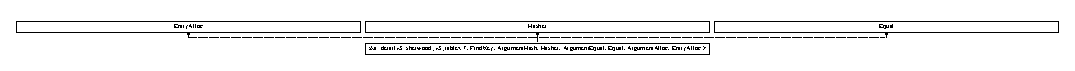
\includegraphics[height=0.512821cm]{classska_1_1detailv3_1_1sherwood__v3__table}
\end{center}
\end{figure}
\subsection*{Classes}
\begin{DoxyCompactItemize}
\item 
struct {\bf convertible\+\_\+to\+\_\+iterator}
\item 
struct {\bf templated\+\_\+iterator}
\end{DoxyCompactItemize}
\subsection*{Public Types}
\begin{DoxyCompactItemize}
\item 
using {\bfseries value\+\_\+type} = T\label{classska_1_1detailv3_1_1sherwood__v3__table_a7a330655116a4689d2773e70c2cce1e9}

\item 
using {\bfseries size\+\_\+type} = size\+\_\+t\label{classska_1_1detailv3_1_1sherwood__v3__table_a3eb8f63db4c50b2320d338080e168256}

\item 
using {\bfseries difference\+\_\+type} = std\+::ptrdiff\+\_\+t\label{classska_1_1detailv3_1_1sherwood__v3__table_a4c2b338c837bd856f7be26bdce7b07d3}

\item 
using {\bfseries hasher} = Argument\+Hash\label{classska_1_1detailv3_1_1sherwood__v3__table_aea93b8f5328be725ee604a83030bac78}

\item 
using {\bfseries key\+\_\+equal} = Argument\+Equal\label{classska_1_1detailv3_1_1sherwood__v3__table_a379f2dfd91ff26565494627c05ff6601}

\item 
using {\bfseries allocator\+\_\+type} = Entry\+Alloc\label{classska_1_1detailv3_1_1sherwood__v3__table_aadeab54e08794b84096f0121ae34b20f}

\item 
using {\bfseries reference} = value\+\_\+type \&\label{classska_1_1detailv3_1_1sherwood__v3__table_a5ceebd69a463a2b22bf0309d94a5845e}

\item 
using {\bfseries const\+\_\+reference} = const value\+\_\+type \&\label{classska_1_1detailv3_1_1sherwood__v3__table_a51ed14b89b4f0a2686ef8f3e2e04e627}

\item 
using {\bfseries pointer} = value\+\_\+type $\ast$\label{classska_1_1detailv3_1_1sherwood__v3__table_ad88e1efd3999da1b71222b1e879c20ce}

\item 
using {\bfseries const\+\_\+pointer} = const value\+\_\+type $\ast$\label{classska_1_1detailv3_1_1sherwood__v3__table_afbb2322b78493266fbe1051532079218}

\item 
using {\bfseries iterator} = {\bf templated\+\_\+iterator}$<$ value\+\_\+type $>$\label{classska_1_1detailv3_1_1sherwood__v3__table_a6e73347b55cd49666d63f765e2afbfbe}

\item 
using {\bfseries const\+\_\+iterator} = {\bf templated\+\_\+iterator}$<$ const value\+\_\+type $>$\label{classska_1_1detailv3_1_1sherwood__v3__table_a381786dc71b4f6f2793ceabe496f7d04}

\end{DoxyCompactItemize}
\subsection*{Public Member Functions}
\begin{DoxyCompactItemize}
\item 
{\bfseries sherwood\+\_\+v3\+\_\+table} (size\+\_\+type bucket\+\_\+count, const Argument\+Hash \&hash=Argument\+Hash(), const Argument\+Equal \&equal=Argument\+Equal(), const Argument\+Alloc \&alloc=Argument\+Alloc())\label{classska_1_1detailv3_1_1sherwood__v3__table_aaa32511bc24a205d8361f0a9ec9dd8d0}

\item 
{\bfseries sherwood\+\_\+v3\+\_\+table} (size\+\_\+type bucket\+\_\+count, const Argument\+Alloc \&alloc)\label{classska_1_1detailv3_1_1sherwood__v3__table_a34f202ef559b7bae86948154c170fe6d}

\item 
{\bfseries sherwood\+\_\+v3\+\_\+table} (size\+\_\+type bucket\+\_\+count, const Argument\+Hash \&hash, const Argument\+Alloc \&alloc)\label{classska_1_1detailv3_1_1sherwood__v3__table_aef224d1aef9b1942b4a89299aee13506}

\item 
{\bfseries sherwood\+\_\+v3\+\_\+table} (const Argument\+Alloc \&alloc)\label{classska_1_1detailv3_1_1sherwood__v3__table_a868295f536ae6050093ef518d59e3213}

\item 
{\footnotesize template$<$typename It $>$ }\\{\bfseries sherwood\+\_\+v3\+\_\+table} (It first, It last, size\+\_\+type bucket\+\_\+count=0, const Argument\+Hash \&hash=Argument\+Hash(), const Argument\+Equal \&equal=Argument\+Equal(), const Argument\+Alloc \&alloc=Argument\+Alloc())\label{classska_1_1detailv3_1_1sherwood__v3__table_acbf66852282c6be341c36de86ca5fd9d}

\item 
{\footnotesize template$<$typename It $>$ }\\{\bfseries sherwood\+\_\+v3\+\_\+table} (It first, It last, size\+\_\+type bucket\+\_\+count, const Argument\+Alloc \&alloc)\label{classska_1_1detailv3_1_1sherwood__v3__table_a81743251db070241f67d26c6490a8f18}

\item 
{\footnotesize template$<$typename It $>$ }\\{\bfseries sherwood\+\_\+v3\+\_\+table} (It first, It last, size\+\_\+type bucket\+\_\+count, const Argument\+Hash \&hash, const Argument\+Alloc \&alloc)\label{classska_1_1detailv3_1_1sherwood__v3__table_a4804a170f10afceacdcaea04f4fd4fce}

\item 
{\bfseries sherwood\+\_\+v3\+\_\+table} (std\+::initializer\+\_\+list$<$ T $>$ il, size\+\_\+type bucket\+\_\+count=0, const Argument\+Hash \&hash=Argument\+Hash(), const Argument\+Equal \&equal=Argument\+Equal(), const Argument\+Alloc \&alloc=Argument\+Alloc())\label{classska_1_1detailv3_1_1sherwood__v3__table_a1e01d0f0bc2bef91111cc3725650c8b9}

\item 
{\bfseries sherwood\+\_\+v3\+\_\+table} (std\+::initializer\+\_\+list$<$ T $>$ il, size\+\_\+type bucket\+\_\+count, const Argument\+Alloc \&alloc)\label{classska_1_1detailv3_1_1sherwood__v3__table_a2b1d486b1600c22433ea307edc9439c7}

\item 
{\bfseries sherwood\+\_\+v3\+\_\+table} (std\+::initializer\+\_\+list$<$ T $>$ il, size\+\_\+type bucket\+\_\+count, const Argument\+Hash \&hash, const Argument\+Alloc \&alloc)\label{classska_1_1detailv3_1_1sherwood__v3__table_ac1274798f4e5daff51a970ce42b33208}

\item 
{\bfseries sherwood\+\_\+v3\+\_\+table} (const {\bf sherwood\+\_\+v3\+\_\+table} \&other)\label{classska_1_1detailv3_1_1sherwood__v3__table_a4ec00a345a75c7c174ce208e8a84606d}

\item 
{\bfseries sherwood\+\_\+v3\+\_\+table} (const {\bf sherwood\+\_\+v3\+\_\+table} \&other, const Argument\+Alloc \&alloc)\label{classska_1_1detailv3_1_1sherwood__v3__table_ac26c91c80f8c1fa92d1a575d63ae924f}

\item 
{\bfseries sherwood\+\_\+v3\+\_\+table} ({\bf sherwood\+\_\+v3\+\_\+table} \&\&other) noexcept\label{classska_1_1detailv3_1_1sherwood__v3__table_a97d71f431ff7b23a666995dc75d0d0bc}

\item 
{\bfseries sherwood\+\_\+v3\+\_\+table} ({\bf sherwood\+\_\+v3\+\_\+table} \&\&other, const Argument\+Alloc \&alloc) noexcept\label{classska_1_1detailv3_1_1sherwood__v3__table_aed772a8cfa891330a49369fcb681ab49}

\item 
{\bf sherwood\+\_\+v3\+\_\+table} \& {\bfseries operator=} (const {\bf sherwood\+\_\+v3\+\_\+table} \&other)\label{classska_1_1detailv3_1_1sherwood__v3__table_aab785e138889f48f453aeb56f9cb3a5f}

\item 
{\bf sherwood\+\_\+v3\+\_\+table} \& {\bfseries operator=} ({\bf sherwood\+\_\+v3\+\_\+table} \&\&other) noexcept\label{classska_1_1detailv3_1_1sherwood__v3__table_a014e26f08f8e3209e26c32b74e602556}

\item 
const allocator\+\_\+type \& {\bfseries get\+\_\+allocator} () const \label{classska_1_1detailv3_1_1sherwood__v3__table_a7a839ab56d3a3a4b658139d313a5d96e}

\item 
const Argument\+Equal \& {\bfseries key\+\_\+eq} () const \label{classska_1_1detailv3_1_1sherwood__v3__table_a5c03df7a5c53d4d1370650071b903753}

\item 
const Argument\+Hash \& {\bfseries hash\+\_\+function} () const \label{classska_1_1detailv3_1_1sherwood__v3__table_a7297e9096c61b4f7eb62d208f68954f4}

\item 
{\bf iterator} {\bfseries begin} ()\label{classska_1_1detailv3_1_1sherwood__v3__table_a1a10add3f012ca6b718e77e22b1a566e}

\item 
{\bf const\+\_\+iterator} {\bfseries begin} () const \label{classska_1_1detailv3_1_1sherwood__v3__table_a0ef070b8634cd1bae3d22b2b461042ad}

\item 
{\bf const\+\_\+iterator} {\bfseries cbegin} () const \label{classska_1_1detailv3_1_1sherwood__v3__table_a4c2d0f8ecdecde9d53fe8c41b201508e}

\item 
{\bf iterator} {\bfseries end} ()\label{classska_1_1detailv3_1_1sherwood__v3__table_a85d44a1eb013c5aadd40c12085c096b4}

\item 
{\bf const\+\_\+iterator} {\bfseries end} () const \label{classska_1_1detailv3_1_1sherwood__v3__table_a70539c3fc38253b7422d87194eb84ee1}

\item 
{\bf const\+\_\+iterator} {\bfseries cend} () const \label{classska_1_1detailv3_1_1sherwood__v3__table_afc653322e9d63349f0009052a8b22887}

\item 
{\bf iterator} {\bfseries find} (const Find\+Key \&key)\label{classska_1_1detailv3_1_1sherwood__v3__table_a4f77659654fc9b95f780d631fcb8ba3c}

\item 
{\bf const\+\_\+iterator} {\bfseries find} (const Find\+Key \&key) const \label{classska_1_1detailv3_1_1sherwood__v3__table_a3f03b08e81232765292c8b5938816256}

\item 
size\+\_\+t {\bfseries count} (const Find\+Key \&key) const \label{classska_1_1detailv3_1_1sherwood__v3__table_a722d57e22f121bab592d749f29f1bc7b}

\item 
std\+::pair$<$ {\bf iterator}, {\bf iterator} $>$ {\bfseries equal\+\_\+range} (const Find\+Key \&key)\label{classska_1_1detailv3_1_1sherwood__v3__table_a3b64e1e928246b3c288b99416d8a7bc3}

\item 
std\+::pair$<$ {\bf const\+\_\+iterator}, {\bf const\+\_\+iterator} $>$ {\bfseries equal\+\_\+range} (const Find\+Key \&key) const \label{classska_1_1detailv3_1_1sherwood__v3__table_aa0742f22c59133513a73edae201d259d}

\item 
{\footnotesize template$<$typename Key , typename... Args$>$ }\\std\+::pair$<$ {\bf iterator}, bool $>$ {\bfseries emplace} (Key \&\&key, Args \&\&...args)\label{classska_1_1detailv3_1_1sherwood__v3__table_a200bc6efadde1c702d43cc409fb19429}

\item 
std\+::pair$<$ {\bf iterator}, bool $>$ {\bfseries insert} (const value\+\_\+type \&value)\label{classska_1_1detailv3_1_1sherwood__v3__table_a60fe276e2e28f1f3a511eaa833cac0ba}

\item 
std\+::pair$<$ {\bf iterator}, bool $>$ {\bfseries insert} (value\+\_\+type \&\&value)\label{classska_1_1detailv3_1_1sherwood__v3__table_a67bfc4de7f7c1ba543663521cdf4b3cb}

\item 
{\footnotesize template$<$typename... Args$>$ }\\{\bf iterator} {\bfseries emplace\+\_\+hint} ({\bf const\+\_\+iterator}, Args \&\&...args)\label{classska_1_1detailv3_1_1sherwood__v3__table_a62aee80e9a17d2ef7e79ca7ac0ca1136}

\item 
{\bf iterator} {\bfseries insert} ({\bf const\+\_\+iterator}, const value\+\_\+type \&value)\label{classska_1_1detailv3_1_1sherwood__v3__table_a8aa6f8b14b1c79e18f9a3d913c626cc7}

\item 
{\bf iterator} {\bfseries insert} ({\bf const\+\_\+iterator}, value\+\_\+type \&\&value)\label{classska_1_1detailv3_1_1sherwood__v3__table_a7155ae2aec75f222c07fb6331a7c7b24}

\item 
{\footnotesize template$<$typename It $>$ }\\void {\bfseries insert} (It begin, It end)\label{classska_1_1detailv3_1_1sherwood__v3__table_ae2e98b3ce956b3457faea3a03171ae5f}

\item 
void {\bfseries insert} (std\+::initializer\+\_\+list$<$ value\+\_\+type $>$ il)\label{classska_1_1detailv3_1_1sherwood__v3__table_acb5b79c6c3184cd718c721e1532f692f}

\item 
void {\bfseries rehash} (size\+\_\+t num\+\_\+buckets)\label{classska_1_1detailv3_1_1sherwood__v3__table_a687ac4c927e81aca2769f7118b4e5c21}

\item 
void {\bfseries reserve} (size\+\_\+t num\+\_\+elements)\label{classska_1_1detailv3_1_1sherwood__v3__table_ad21abfcf8f6cab5268f777b76337c549}

\item 
{\bf convertible\+\_\+to\+\_\+iterator} {\bfseries erase} ({\bf const\+\_\+iterator} to\+\_\+erase)\label{classska_1_1detailv3_1_1sherwood__v3__table_af240d7373ecbeed71ca3eddc7b37d669}

\item 
{\bf iterator} {\bfseries erase} ({\bf const\+\_\+iterator} begin\+\_\+it, {\bf const\+\_\+iterator} end\+\_\+it)\label{classska_1_1detailv3_1_1sherwood__v3__table_ac2301f42fb2102ae6d39188bc1f3aed3}

\item 
size\+\_\+t {\bfseries erase} (const Find\+Key \&key)\label{classska_1_1detailv3_1_1sherwood__v3__table_a3a359b9c62c5db91a4c6474e7df64c9b}

\item 
void {\bfseries clear} ()\label{classska_1_1detailv3_1_1sherwood__v3__table_a8610b4acfeb3dea476ad95bf4bdd743c}

\item 
void {\bfseries shrink\+\_\+to\+\_\+fit} ()\label{classska_1_1detailv3_1_1sherwood__v3__table_a5dd497165958e5445a925113d6f7ab32}

\item 
void {\bfseries swap} ({\bf sherwood\+\_\+v3\+\_\+table} \&other)\label{classska_1_1detailv3_1_1sherwood__v3__table_a6b03fb89708db39b37a97bdcc62dac66}

\item 
size\+\_\+t {\bfseries size} () const \label{classska_1_1detailv3_1_1sherwood__v3__table_aa6159ec66e44afb5ceaf5c724588aeb8}

\item 
size\+\_\+t {\bfseries max\+\_\+size} () const \label{classska_1_1detailv3_1_1sherwood__v3__table_a90d1cc3ed7257d54a5ab15d1ee2b8ca8}

\item 
size\+\_\+t {\bfseries bucket\+\_\+count} () const \label{classska_1_1detailv3_1_1sherwood__v3__table_ab6ca95ddf24486c623e756f88603dc31}

\item 
size\+\_\+type {\bfseries max\+\_\+bucket\+\_\+count} () const \label{classska_1_1detailv3_1_1sherwood__v3__table_a04e8b09b65d4d0894407bd8879f5c2fb}

\item 
size\+\_\+t {\bfseries bucket} (const Find\+Key \&key) const \label{classska_1_1detailv3_1_1sherwood__v3__table_a42cc5cecfbb20230ee189f28b65fca7c}

\item 
float {\bfseries load\+\_\+factor} () const \label{classska_1_1detailv3_1_1sherwood__v3__table_a63a605a0c204472c3018da2921b87cdc}

\item 
void {\bfseries max\+\_\+load\+\_\+factor} (float value)\label{classska_1_1detailv3_1_1sherwood__v3__table_adc1c8ab152d3934157b3d22a71dcab3e}

\item 
float {\bfseries max\+\_\+load\+\_\+factor} () const \label{classska_1_1detailv3_1_1sherwood__v3__table_a213a3854ab4aab689ec301185f1e1446}

\item 
bool {\bfseries empty} () const \label{classska_1_1detailv3_1_1sherwood__v3__table_a4957a0b7d6c8f720efbaf7d310feb60e}

\end{DoxyCompactItemize}
\subsection*{Private Types}
\begin{DoxyCompactItemize}
\item 
using {\bfseries Entry} = {\bf detailv3\+::sherwood\+\_\+v3\+\_\+entry}$<$ T $>$\label{classska_1_1detailv3_1_1sherwood__v3__table_a73c15a0a60030b8f148d40f1aecab2d8}

\item 
using {\bfseries Allocator\+Traits} = std\+::allocator\+\_\+traits$<$ Entry\+Alloc $>$\label{classska_1_1detailv3_1_1sherwood__v3__table_ac1603d09ba4eb53eb927734a7b640ede}

\item 
using {\bfseries Entry\+Pointer} = typename Allocator\+Traits\+::pointer\label{classska_1_1detailv3_1_1sherwood__v3__table_a6e8384a98f42d8d39b44f0bfcad73be5}

\item 
using {\bfseries Default\+Table} = {\bf detailv3\+::\+Entry\+Default\+Table}$<$ T $>$\label{classska_1_1detailv3_1_1sherwood__v3__table_aa9c5b669279d50c3439ab203bc30ab7a}

\end{DoxyCompactItemize}
\subsection*{Private Member Functions}
\begin{DoxyCompactItemize}
\item 
size\+\_\+t {\bfseries num\+\_\+buckets\+\_\+for\+\_\+reserve} (size\+\_\+t num\+\_\+elements) const \label{classska_1_1detailv3_1_1sherwood__v3__table_a227f0bd044907bd39408a98928cf055a}

\item 
void {\bfseries rehash\+\_\+for\+\_\+other\+\_\+container} (const {\bf sherwood\+\_\+v3\+\_\+table} \&other)\label{classska_1_1detailv3_1_1sherwood__v3__table_ab743f94bcf0887332f64489c93b10420}

\item 
void {\bfseries swap\+\_\+pointers} ({\bf sherwood\+\_\+v3\+\_\+table} \&other)\label{classska_1_1detailv3_1_1sherwood__v3__table_a2304a8c084c7649ad6a56f57dd509bc8}

\item 
{\footnotesize template$<$typename Key , typename... Args$>$ }\\{\bfseries S\+K\+A\+\_\+\+N\+O\+I\+N\+L\+I\+NE} (std\+::pair$<$ {\bf iterator}, bool $>$) emplace\+\_\+new\+\_\+key(int8\+\_\+t distance\+\_\+from\+\_\+desired\label{classska_1_1detailv3_1_1sherwood__v3__table_ab834eb352e96c51e3c948284fe6db5e5}

\item 
{\bfseries if} (num\+\_\+slots\+\_\+minus\+\_\+one==0$\vert$$\vert$distance\+\_\+from\+\_\+desired==max\+\_\+lookups$\vert$$\vert$static\+\_\+cast$<$ double $>$(num\+\_\+elements+1)/static\+\_\+cast$<$ double $>$(bucket\+\_\+count()) $>$ \+\_\+max\+\_\+load\+\_\+factor)\label{classska_1_1detailv3_1_1sherwood__v3__table_a11a2fdb1a7b222ff2e3e568b6cb65fd6}

\item 
else {\bfseries if} (current\+\_\+entry-\/$>$is\+\_\+empty())\label{classska_1_1detailv3_1_1sherwood__v3__table_a6ae64d4164e3b374d0a45813b5602479}

\item 
value\+\_\+type {\bfseries to\+\_\+insert} (std\+::forward$<$ Key $>$(key), std\+::forward$<$ Args $>$(args)...)\label{classska_1_1detailv3_1_1sherwood__v3__table_a997dd4841a0c18af664c940807125175}

\item 
{\bfseries swap} (distance\+\_\+from\+\_\+desired, current\+\_\+entry-\/$>$distance\+\_\+from\+\_\+desired)\label{classska_1_1detailv3_1_1sherwood__v3__table_ac0c961acbfbb68270133a74cf0ebf101}

\item 
{\bfseries swap} (to\+\_\+insert, current\+\_\+entry-\/$>$value)\label{classska_1_1detailv3_1_1sherwood__v3__table_a87f3c74a2acbddcc8d89da67227ebf44}

\item 
{\bfseries for} (++distance\+\_\+from\+\_\+desired,++current\+\_\+entry;;++current\+\_\+entry)\label{classska_1_1detailv3_1_1sherwood__v3__table_a506dd91bb8f538c62f13a2e253501698}

\item 
void {\bfseries grow} ()\label{classska_1_1detailv3_1_1sherwood__v3__table_aae7057e0e02182ebfb6f1af6eafb8c7a}

\item 
void {\bfseries deallocate\+\_\+data} (Entry\+Pointer begin, size\+\_\+t num\+\_\+slots\+\_\+minus\+\_\+one, int8\+\_\+t max\+\_\+lookups)\label{classska_1_1detailv3_1_1sherwood__v3__table_a1011f360b048cebd083665d2f167d5e2}

\item 
void {\bfseries reset\+\_\+to\+\_\+empty\+\_\+state} ()\label{classska_1_1detailv3_1_1sherwood__v3__table_a7bdbcd192ce21a8e9387d0f1813c1df7}

\item 
{\footnotesize template$<$typename U $>$ }\\size\+\_\+t {\bfseries hash\+\_\+object} (const U \&key)\label{classska_1_1detailv3_1_1sherwood__v3__table_af8223a9d5081379c092eae7d28f40ea2}

\item 
{\footnotesize template$<$typename U $>$ }\\size\+\_\+t {\bfseries hash\+\_\+object} (const U \&key) const \label{classska_1_1detailv3_1_1sherwood__v3__table_a53c778c0f19e6068493caa1eef933949}

\item 
{\footnotesize template$<$typename L , typename R $>$ }\\bool {\bfseries compares\+\_\+equal} (const L \&lhs, const R \&rhs)\label{classska_1_1detailv3_1_1sherwood__v3__table_a793b987a5fe980380c3747275022cb91}

\end{DoxyCompactItemize}
\subsection*{Static Private Member Functions}
\begin{DoxyCompactItemize}
\item 
static int8\+\_\+t {\bfseries compute\+\_\+max\+\_\+lookups} (size\+\_\+t num\+\_\+buckets)\label{classska_1_1detailv3_1_1sherwood__v3__table_aee430fb4a4044b4788a9610d866b9083}

\end{DoxyCompactItemize}
\subsection*{Private Attributes}
\begin{DoxyCompactItemize}
\item 
Entry\+Pointer {\bfseries entries} = const\+\_\+cast$<${\bf Entry} $\ast$$>$(reinterpret\+\_\+cast$<$const {\bf Entry} $\ast$$>$(Default\+Table\+::table))\label{classska_1_1detailv3_1_1sherwood__v3__table_ae1589776281f4e41cce8480108528966}

\item 
size\+\_\+t {\bfseries num\+\_\+slots\+\_\+minus\+\_\+one} = 0\label{classska_1_1detailv3_1_1sherwood__v3__table_a429f76f8c4db79ffb508c771af707bec}

\item 
{\bf Hash\+Policy\+Selector}$<$ Argument\+Hash $>$\+::type {\bfseries hash\+\_\+policy}\label{classska_1_1detailv3_1_1sherwood__v3__table_a42bdf8be15a2681dc756b7ea90e7df54}

\item 
int8\+\_\+t {\bfseries max\+\_\+lookups} = detailv3\+::min\+\_\+lookups -\/ 1\label{classska_1_1detailv3_1_1sherwood__v3__table_afad29da26ad8cbd730d75fd420d37ea8}

\item 
float {\bfseries \+\_\+max\+\_\+load\+\_\+factor} = 0.\+5f\label{classska_1_1detailv3_1_1sherwood__v3__table_a99df4bd36240137cc818a50719e8e731}

\item 
size\+\_\+t {\bfseries num\+\_\+elements} = 0\label{classska_1_1detailv3_1_1sherwood__v3__table_a2b9f43ccdb9c9b59430b59249b035c4b}

\item 
Entry\+Pointer {\bfseries current\+\_\+entry}\label{classska_1_1detailv3_1_1sherwood__v3__table_a9769bdcca4c87de6a37cfcbcd64bb918}

\item 
Entry\+Pointer Key \&\& {\bfseries key}\label{classska_1_1detailv3_1_1sherwood__v3__table_ad0be4cf3e612706ff6f5af9cebf73321}

\item 
Entry\+Pointer Key Args \&\& {\bfseries args}
\item 
{\bf iterator} {\bfseries result} = \{ current\+\_\+entry \}\label{classska_1_1detailv3_1_1sherwood__v3__table_aed2a992cbbfa3ef56e6dc2fbbfcac8bb}

\end{DoxyCompactItemize}


\subsection{Member Data Documentation}
\index{ska\+::detailv3\+::sherwood\+\_\+v3\+\_\+table@{ska\+::detailv3\+::sherwood\+\_\+v3\+\_\+table}!args@{args}}
\index{args@{args}!ska\+::detailv3\+::sherwood\+\_\+v3\+\_\+table@{ska\+::detailv3\+::sherwood\+\_\+v3\+\_\+table}}
\subsubsection[{args}]{\setlength{\rightskip}{0pt plus 5cm}template$<$typename T, typename Find\+Key, typename Argument\+Hash, typename Hasher, typename Argument\+Equal, typename Equal, typename Argument\+Alloc, typename Entry\+Alloc$>$ Entry\+Pointer Key Args\&\& {\bf ska\+::detailv3\+::sherwood\+\_\+v3\+\_\+table}$<$ T, Find\+Key, Argument\+Hash, Hasher, Argument\+Equal, Equal, Argument\+Alloc, Entry\+Alloc $>$\+::args\hspace{0.3cm}{\ttfamily [private]}}\label{classska_1_1detailv3_1_1sherwood__v3__table_a931fdaa54363e9cd5ac181a4ac7e3af0}
{\bfseries Initial value\+:}
\begin{DoxyCode}
\{
        \textcolor{keyword}{using} std::swap
\end{DoxyCode}


The documentation for this class was generated from the following file\+:\begin{DoxyCompactItemize}
\item 
/home/felipe/\+Desktop/vdsproject/vdscp\+\_\+04/src/flat\+\_\+hash\+\_\+map.\+hpp\end{DoxyCompactItemize}

\section{skip\+\_\+p\+:\+:skip\+\_\+grammar$<$ Iterator $>$ Struct Template Reference}
\label{structskip__p_1_1skip__grammar}\index{skip\+\_\+p\+::skip\+\_\+grammar$<$ Iterator $>$@{skip\+\_\+p\+::skip\+\_\+grammar$<$ Iterator $>$}}
Inheritance diagram for skip\+\_\+p\+:\+:skip\+\_\+grammar$<$ Iterator $>$\+:\begin{figure}[H]
\begin{center}
\leavevmode
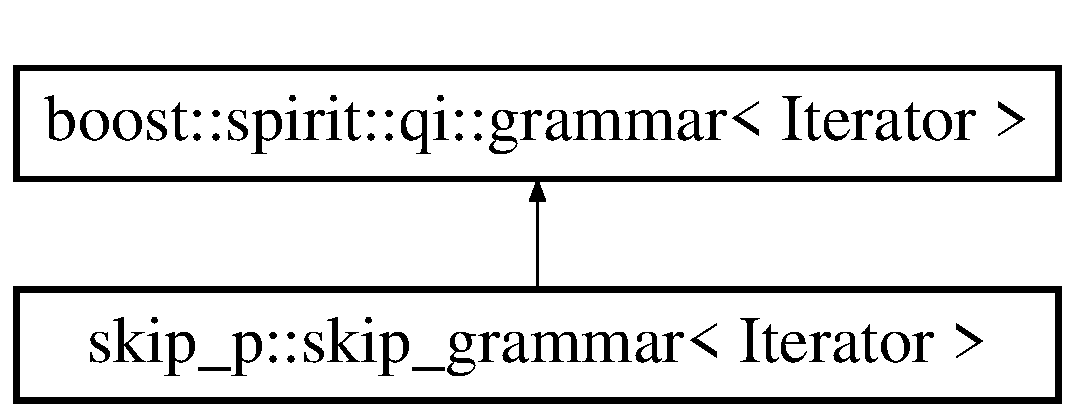
\includegraphics[height=2.000000cm]{structskip__p_1_1skip__grammar}
\end{center}
\end{figure}
\subsection*{Public Attributes}
\begin{DoxyCompactItemize}
\item 
qi\+::rule$<$ Iterator $>$ {\bfseries skip\+\_\+}\label{structskip__p_1_1skip__grammar_ae0feb7886ff25cd5363083242bb41239}

\item 
qi\+::rule$<$ Iterator $>$ {\bfseries line\+\_\+comment\+\_\+}\label{structskip__p_1_1skip__grammar_a1cf07ff2e793ae00e4181b23ea9ace2c}

\end{DoxyCompactItemize}


The documentation for this struct was generated from the following file\+:\begin{DoxyCompactItemize}
\item 
/home/felipe/\+Desktop/vdsproject/vdscp\+\_\+04/src/bench/skip\+\_\+parser.\+hpp\end{DoxyCompactItemize}

\section{Syntax\+Exception Class Reference}
\label{classSyntaxException}\index{Syntax\+Exception@{Syntax\+Exception}}


This exception should be thrown when the file does not have the proper syntax.  




{\ttfamily \#include $<$bench\+\_\+circuit\+\_\+manager.\+hpp$>$}

Inheritance diagram for Syntax\+Exception\+:\begin{figure}[H]
\begin{center}
\leavevmode
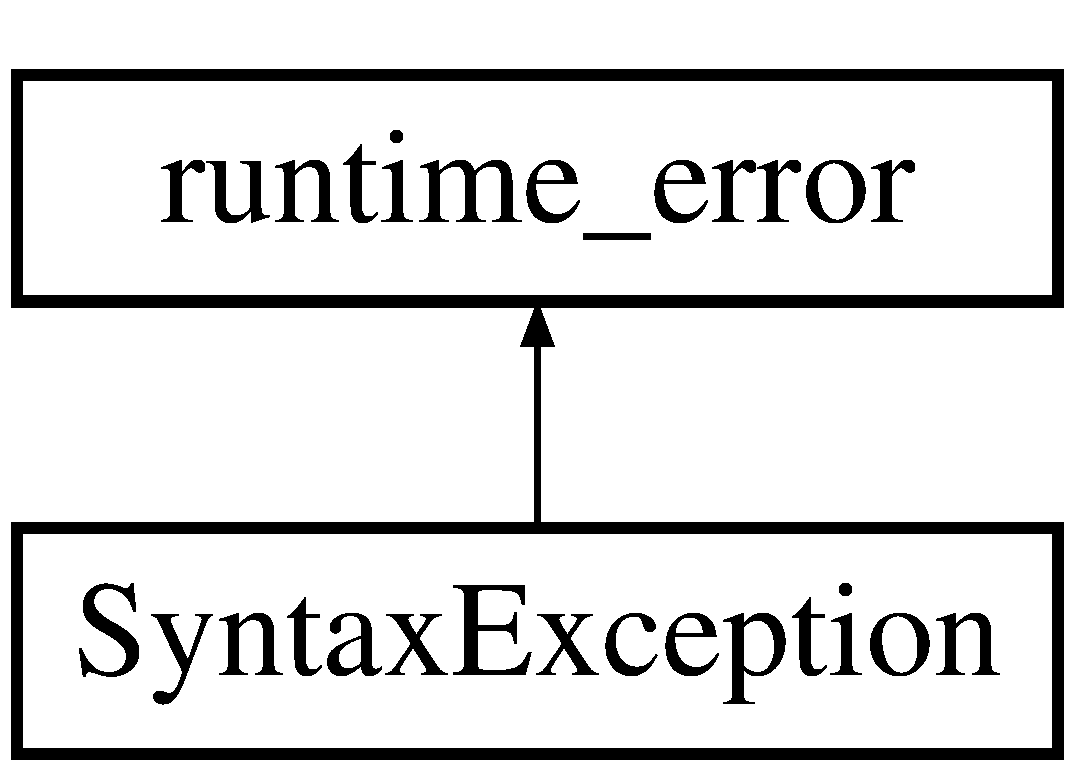
\includegraphics[height=2.000000cm]{classSyntaxException}
\end{center}
\end{figure}
\subsection*{Public Member Functions}
\begin{DoxyCompactItemize}
\item 
{\bfseries Syntax\+Exception} (const std\+::string \&message)\label{classSyntaxException_a017056b4446f0770e521c995c661aa25}

\end{DoxyCompactItemize}


\subsection{Detailed Description}
This exception should be thrown when the file does not have the proper syntax. 

The documentation for this class was generated from the following file\+:\begin{DoxyCompactItemize}
\item 
/import/home/vdscp04/\+Luiz/vdscp\+\_\+04/src/bench/bench\+\_\+circuit\+\_\+manager.\+hpp\end{DoxyCompactItemize}

\section{ska\+:\+:detailv3\+:\+:sherwood\+\_\+v3\+\_\+table$<$ T, Find\+Key, Argument\+Hash, Hasher, Argument\+Equal, Equal, Argument\+Alloc, Entry\+Alloc $>$\+:\+:templated\+\_\+iterator$<$ Value\+Type $>$ Struct Template Reference}
\label{structska_1_1detailv3_1_1sherwood__v3__table_1_1templated__iterator}\index{ska\+::detailv3\+::sherwood\+\_\+v3\+\_\+table$<$ T, Find\+Key, Argument\+Hash, Hasher, Argument\+Equal, Equal, Argument\+Alloc, Entry\+Alloc $>$\+::templated\+\_\+iterator$<$ Value\+Type $>$@{ska\+::detailv3\+::sherwood\+\_\+v3\+\_\+table$<$ T, Find\+Key, Argument\+Hash, Hasher, Argument\+Equal, Equal, Argument\+Alloc, Entry\+Alloc $>$\+::templated\+\_\+iterator$<$ Value\+Type $>$}}
\subsection*{Public Types}
\begin{DoxyCompactItemize}
\item 
using {\bfseries iterator\+\_\+category} = std\+::forward\+\_\+iterator\+\_\+tag\label{structska_1_1detailv3_1_1sherwood__v3__table_1_1templated__iterator_a11da233839fedaeb7c04de3b9ceba01c}

\item 
using {\bfseries value\+\_\+type} = Value\+Type\label{structska_1_1detailv3_1_1sherwood__v3__table_1_1templated__iterator_ae5beca4c34ba34f8f72db61e70c32768}

\item 
using {\bfseries difference\+\_\+type} = ptrdiff\+\_\+t\label{structska_1_1detailv3_1_1sherwood__v3__table_1_1templated__iterator_a5ead70f703f844442fc7d6f99501009b}

\item 
using {\bfseries pointer} = Value\+Type $\ast$\label{structska_1_1detailv3_1_1sherwood__v3__table_1_1templated__iterator_a86b20ddef58240ee2425e940042468ce}

\item 
using {\bfseries reference} = Value\+Type \&\label{structska_1_1detailv3_1_1sherwood__v3__table_1_1templated__iterator_a713c0031feacd2b96445864d1640b3a6}

\end{DoxyCompactItemize}
\subsection*{Public Member Functions}
\begin{DoxyCompactItemize}
\item 
{\bf templated\+\_\+iterator} \& {\bfseries operator++} ()\label{structska_1_1detailv3_1_1sherwood__v3__table_1_1templated__iterator_ae2a915085c4b6c2a9c49052473463782}

\item 
{\bf templated\+\_\+iterator} {\bfseries operator++} (int)\label{structska_1_1detailv3_1_1sherwood__v3__table_1_1templated__iterator_a0abeb60414eddc1c05c44294be92a2a6}

\item 
Value\+Type \& {\bfseries operator$\ast$} () const \label{structska_1_1detailv3_1_1sherwood__v3__table_1_1templated__iterator_a48db2a1e7d3d66238c644af66691c85b}

\item 
Value\+Type $\ast$ {\bfseries operator-\/$>$} () const \label{structska_1_1detailv3_1_1sherwood__v3__table_1_1templated__iterator_aab3e2443f9c8f7b24b61ff58533c4519}

\item 
{\bfseries operator templated\+\_\+iterator$<$ const value\+\_\+type $>$} () const \label{structska_1_1detailv3_1_1sherwood__v3__table_1_1templated__iterator_ace521f6a78b76532bbd1a9ce94bc62c4}

\end{DoxyCompactItemize}
\subsection*{Public Attributes}
\begin{DoxyCompactItemize}
\item 
Entry\+Pointer {\bfseries current} = Entry\+Pointer()\label{structska_1_1detailv3_1_1sherwood__v3__table_1_1templated__iterator_a8537396973141815a65488447b1aa627}

\end{DoxyCompactItemize}
\subsection*{Friends}
\begin{DoxyCompactItemize}
\item 
bool {\bfseries operator==} (const {\bf templated\+\_\+iterator} \&lhs, const {\bf templated\+\_\+iterator} \&rhs)\label{structska_1_1detailv3_1_1sherwood__v3__table_1_1templated__iterator_a4f593a758a735615a7b8775a829d907b}

\item 
bool {\bfseries operator!=} (const {\bf templated\+\_\+iterator} \&lhs, const {\bf templated\+\_\+iterator} \&rhs)\label{structska_1_1detailv3_1_1sherwood__v3__table_1_1templated__iterator_adba9c494ff40b17dd700f1d612ce196a}

\end{DoxyCompactItemize}


The documentation for this struct was generated from the following file\+:\begin{DoxyCompactItemize}
\item 
/home/felipe/\+Desktop/vdsproject/vdscp\+\_\+04/src/flat\+\_\+hash\+\_\+map.\+hpp\end{DoxyCompactItemize}

\section{Class\+Project\+:\+:Text\+Bdd\+Dumper Class Reference}
\label{classClassProject_1_1TextBddDumper}\index{Class\+Project\+::\+Text\+Bdd\+Dumper@{Class\+Project\+::\+Text\+Bdd\+Dumper}}
Inheritance diagram for Class\+Project\+:\+:Text\+Bdd\+Dumper\+:\begin{figure}[H]
\begin{center}
\leavevmode
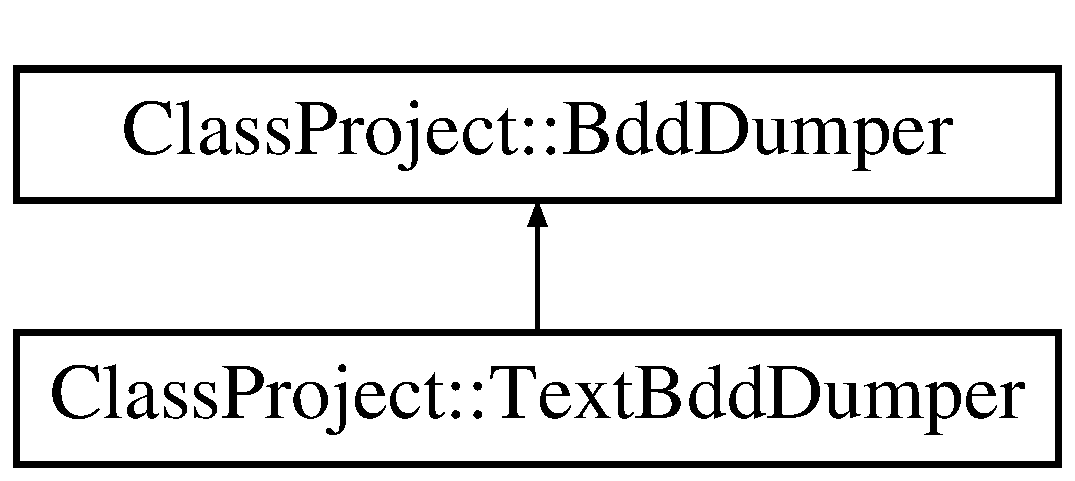
\includegraphics[height=2.000000cm]{classClassProject_1_1TextBddDumper}
\end{center}
\end{figure}
\subsection*{Public Member Functions}
\begin{DoxyCompactItemize}
\item 
{\bfseries Text\+Bdd\+Dumper} ({\bf Manager} \&mgr)\label{classClassProject_1_1TextBddDumper_ae6d584f67f73ba58ac5a146e9921d2da}

\item 
virtual void {\bfseries dump} (const B\+D\+D\+\_\+\+ID \&root, std\+::ostream \&out)\label{classClassProject_1_1TextBddDumper_a24d38ffd14716206cb8d24937d06876e}

\end{DoxyCompactItemize}
\subsection*{Private Attributes}
\begin{DoxyCompactItemize}
\item 
{\bf Manager} \& {\bfseries m\+Mgr}\label{classClassProject_1_1TextBddDumper_a9c49ecb488d85d0ac8a9f3120a65cead}

\end{DoxyCompactItemize}


The documentation for this class was generated from the following files\+:\begin{DoxyCompactItemize}
\item 
/home/felipe/\+Desktop/vdsproject/vdscp\+\_\+04/src/bench/Dumper.\+h\item 
/home/felipe/\+Desktop/vdsproject/vdscp\+\_\+04/src/bench/Dumper.\+cpp\end{DoxyCompactItemize}

%--- End generated contents ---

% Index
\backmatter
\newpage
\phantomsection
\clearemptydoublepage
\addcontentsline{toc}{chapter}{Index}
\printindex

\end{document}
